\documentclass[a4paper,14pt,oneside,openany]{memoir}

%%% Задаем поля, отступы и межстрочный интервал %%%

\usepackage[left=30mm, right=15mm, top=20mm, bottom=20mm]{geometry} % Пакет geometry с аргументами для определения полей
\pagestyle{plain} % Убираем стандарные для данного класса верхние колонтитулы с заголовком текущей главы, оставляем только номер страницы снизу по центру
\parindent=1.25cm % Абзацный отступ 1.25 см, приблизительно равно пяти знакам, как по ГОСТ
\usepackage{indentfirst} % Добавляем отступ к первому абзацу
%\linespread{1.3} % Межстрочный интервал (наиболее близко к вордовскому полуторному) - тут вместо этого используется команда OnehalfSpacing*

%%% Задаем языковые параметры и шрифт %%%

\usepackage[english, russian]{babel}                % Настройки для русского языка как основного в тексте
\babelfont{rm}{Times New Roman}                     % TMR в качестве базового roman-щрифта

%%% Задаем стиль заголовков и подзаголовков в тексте %%%

\setsecnumdepth{subsection} % Номера разделов считать до третьего уровня включительно, т.е. нумеруются только главы, секции, подсекции
\renewcommand*{\chapterheadstart}{} % Переопределяем команду, задающую отступ над заголовком, чтобы отступа не было
\renewcommand*{\printchaptername}{} % Переопределяем команду, печатающую слово "Глава", чтобы оно не печалось
%\renewcommand*{\printchapternum}{} % То же самое для номера главы - тут не надо, номер главы оставляем
\renewcommand*{\chapnumfont}{\normalfont\bfseries} % Меняем стиль шрифта для номера главы: нормальный размер, полужирный
\renewcommand*{\afterchapternum}{\hspace{1em}} % Меняем разделитель между номером главы и названием
\renewcommand*{\printchaptertitle}{\normalfont\bfseries\centering\MakeUppercase} % Меняем стиль написания для заголовка главы: нормальный размер, полужирный, центрированный, заглавными буквами
\setbeforesecskip{20pt} % Задаем отступ перед заголовком секции
\setaftersecskip{20pt} % Ставим такой же отступ после заголовка секции
\setsecheadstyle{\raggedright\normalfont\bfseries} % Меняем стиль написания для заголовка секции: выравнивание по правому краю без переносов, нормальный размер, полужирный
\setbeforesubsecskip{20pt} % Задаем отступ перед заголовком подсекции
\setaftersubsecskip{20pt} % Ставим такой же отступ после заголовка подсекции
\setsubsecheadstyle{\raggedright\normalfont\bfseries}  % Меняем стиль написания для заголовка подсекции: выравнивание по правому краю без переносов, нормальный размер, полужирный

%%% Задаем параметры оглавления %%%

\addto\captionsrussian{\renewcommand\contentsname{Содержание}} % Меняем слово "Оглавление" на "Содержание"
\setrmarg{2.55em plus1fil} % Запрещаем переносы слов в оглавлении
%\setlength{\cftbeforechapterskip}{0pt} % Эта команда убирает интервал между заголовками глав - тут не надо, так красивее смотрится
\renewcommand{\aftertoctitle}{\afterchaptertitle \vspace{-\cftbeforechapterskip}} % Делаем отступ между словом "Содержание" и первой строкой таким же, как у заголовков глав
%\renewcommand*{\chapternumberline}[1]{} % Делаем так, чтобы номер главы не печатался - тут не надо
\renewcommand*{\cftchapternumwidth}{1.5em} % Ставим подходящий по размеру разделитель между номером главы и самим заголовком
\renewcommand*{\cftchapterfont}{\normalfont\MakeUppercase} % Названия глав обычным шрифтом заглавными буквами
\renewcommand*{\cftchapterpagefont}{\normalfont} % Номера страниц обычным шрифтом
\renewcommand*{\cftchapterdotsep}{\cftdotsep} % Делаем точки до номера страницы после названий глав
\renewcommand*{\cftdotsep}{1} % Задаем расстояние между точками
\renewcommand*{\cftchapterleader}{\cftdotfill{\cftchapterdotsep}} % Делаем точки стандартной формы (по умолчанию они "жирные")
\maxtocdepth{subsection} % В оглавление попадают только разделы первыхтрех уровней: главы, секции и подсекции

%%% Выравнивание и переносы %%%

%% http://tex.stackexchange.com/questions/241343/what-is-the-meaning-of-fussy-sloppy-emergencystretch-tolerance-hbadness
%% http://www.latex-community.org/forum/viewtopic.php?p=70342#p70342
\tolerance 1414
\hbadness 1414
\emergencystretch 1.5em                             % В случае проблем регулировать в первую очередь
\hfuzz 0.3pt
\vfuzz \hfuzz
%\dbottom
%\sloppy                                            % Избавляемся от переполнений
\clubpenalty=10000                                  % Запрещаем разрыв страницы после первой строки абзаца
\widowpenalty=10000                                 % Запрещаем разрыв страницы после последней строки абзаца
\brokenpenalty=4991                                 % Ограничение на разрыв страницы, если строка заканчивается переносом

%%% Объясняем компилятору, какие буквы русского алфавита можно использовать в перечислениях (подрисунках и нумерованных списках) %%%
%%% По ГОСТ нельзя использовать буквы ё, з, й, о, ч, ь, ы, ъ %%%
%%% Здесь также переопределены заглавные буквы, хотя в принципе они в документе не используются %%%

\makeatletter
    \def\russian@Alph#1{\ifcase#1\or
       А\or Б\or В\or Г\or Д\or Е\or Ж\or
       И\or К\or Л\or М\or Н\or
       П\or Р\or С\or Т\or У\or Ф\or Х\or
       Ц\or Ш\or Щ\or Э\or Ю\or Я\else\xpg@ill@value{#1}{russian@Alph}\fi}
    \def\russian@alph#1{\ifcase#1\or
       а\or б\or в\or г\or д\or е\or ж\or
       и\or к\or л\or м\or н\or
       п\or р\or с\or т\or у\or ф\or х\or
       ц\or ш\or щ\or э\or ю\or я\else\xpg@ill@value{#1}{russian@alph}\fi}
\makeatother

%%% Задаем параметры оформления рисунков и таблиц %%%

\usepackage{graphicx, caption, subcaption} % Подгружаем пакеты для работы с графикой и настройки подписей
\graphicspath{{images/}} % Определяем папку с рисунками
\captionsetup[figure]{font=small, width=\textwidth, name=Рисунок, justification=centering} % Задаем параметры подписей к рисункам: маленький шрифт (в данном случае 12pt), ширина равна ширине текста, полнотекстовая надпись "Рисунок", выравнивание по центру
\captionsetup[subfigure]{font=small} % Индексы подрисунков а), б) и так далее тоже шрифтом 12pt (по умолчанию делает еще меньше)
\captionsetup[table]{singlelinecheck=false,font=small,width=\textwidth,justification=justified} % Задаем параметры подписей к таблицам: запрещаем переносы, маленький шрифт (в данном случае 12pt), ширина равна ширине текста, выравнивание по ширине
\captiondelim{ --- } % Разделителем между номером рисунка/таблицы и текстом в подписи является длинное тире
\setkeys{Gin}{width=\textwidth} % По умолчанию размер всех добавляемых рисунков будет подгоняться под ширину текста
\renewcommand{\thesubfigure}{\asbuk{subfigure}} % Нумерация подрисунков строчными буквами кириллицы
%\setlength{\abovecaptionskip}{0pt} % Отбивка над подписью - тут не меняем
%\setlength{\belowcaptionskip}{0pt} % Отбивка под подписью - тут не меняем
\usepackage[section]{placeins} % Объекты типа float (рисунки/таблицы) не вылезают за границы секциии, в которой они объявлены

%%% Задаем параметры ссылок и гиперссылок %%% 

\usepackage{hyperref}                               % Подгружаем нужный пакет
\hypersetup{
    colorlinks=true,                                % Все ссылки и гиперссылки цветные
    linktoc=all,                                    % В оглавлении ссылки подключатся для всех отображаемых уровней
    linktocpage=true,                               % Ссылка - только номер страницы, а не весь заголовок (так выглядит аккуратнее)
    linkcolor=red,                                  % Цвет ссылок и гиперссылок - красный
    citecolor=red                                   % Цвет цитировний - красный
}

%%% Настраиваем отображение списков %%%

\usepackage{enumitem}                               % Подгружаем пакет для гибкой настройки списков
\renewcommand*{\labelitemi}{\normalfont{--}}        % В ненумерованных списках для пунктов используем короткое тире
\makeatletter
    \AddEnumerateCounter{\asbuk}{\russian@alph}     % Объясняем пакету enumitem, как использовать asbuk
\makeatother
\renewcommand{\labelenumii}{\asbuk{enumii})}        % Кириллица для второго уровня нумерации
\renewcommand{\labelenumiii}{\arabic{enumiii})}     % Арабские цифры для третьего уровня нумерации
\setlist{noitemsep, leftmargin=*}                   % Убираем интервалы между пунками одного уровня в списке
\setlist[1]{labelindent=\parindent}                 % Отступ у пунктов списка равен абзацному отступу
\setlist[2]{leftmargin=\parindent}                  % Плюс еще один такой же отступ для следующего уровня
\setlist[3]{leftmargin=\parindent}                  % И еще один для третьего уровня

%%% Счетчики для нумерации объектов %%%

\counterwithout{figure}{chapter}                    % Сквозная нумерация рисунков по документу
\counterwithout{equation}{chapter}                  % Сквозная нумерация математических выражений по документу
\counterwithout{table}{chapter}                     % Сквозная нумерация таблиц по документу

%%% Реализация библиографии пакетами biblatex и biblatex-gost с использованием движка biber %%%

\usepackage{csquotes} % Пакет для оформления сложных блоков цитирования (biblatex рекомендует его подключать)
\usepackage[%
backend=biber,                                      % Движок
bibencoding=utf8,                                   % Кодировка bib-файла
sorting=none,                                       % Настройка сортировки списка литературы
style=gost-numeric,                                 % Стиль цитирования и библиографии по ГОСТ
language=auto,                                      % Язык для каждой библиографической записи задается отдельно
autolang=other,                                     % Поддержка многоязычной библиографии
sortcites=true,                                     % Если в квадратных скобках несколько ссылок, то отображаться будут отсортированно
movenames=false,                                    % Не перемещать имена, они всегда в начале библиографической записи
maxnames=5,                                         % Максимальное отображаемое число авторов
minnames=3,                                         % До скольки сокращать число авторов, если их больше максимума
doi=false,                                          % Не отображать ссылки на DOI
isbn=false,                                         % Не показывать ISBN, ISSN, ISRN
]{biblatex}[2016/09/17]
\DeclareDelimFormat{bibinitdelim}{}                 % Убираем пробел между инициалами (Иванов И.И. вместо Иванов И. И.)
\addbibresource{biba.bib}                           % Определяем файл с библиографией

%%% Скрипт, который автоматически подбирает язык (и, следовательно, формат) для каждой библиографической записи %%%
%%% Если в названии работы есть кириллица - меняем значение поля langid на russian %%%
%%% Все оставшиеся пустые места в поле langid заменяем на english %%%

\DeclareSourcemap{
  \maps[datatype=bibtex]{
    \map{
        \step[fieldsource=title, match=\regexp{^\P{Cyrillic}*\p{Cyrillic}.*}, final]
        \step[fieldset=langid, fieldvalue={russian}]
    }
    \map{
        \step[fieldset=langid, fieldvalue={english}]
    }
  }
}

%%% Прочие пакеты для расширения функционала %%%

\usepackage{longtable,ltcaption}                    % Длинные таблицы
\usepackage{multirow,makecell}                      % Улучшенное форматирование таблиц
\usepackage{booktabs}                               % Еще один пакет для красивых таблиц
\usepackage{soulutf8}                               % Поддержка переносоустойчивых подчёркиваний и зачёркиваний
\usepackage{icomma}                                 % Запятая в десятичных дробях
\usepackage{hyphenat}                               % Для красивых переносов
\usepackage{textcomp}                               % Поддержка "сложных" печатных символов типа значков иены, копирайта и т.д.
\usepackage[version=4]{mhchem}                      % Красивые химические уравнения
\usepackage{amsmath}                                % Усовершенствование отображения математических выражений 
\usepackage{listings}
\usepackage{xcolor}
\usepackage{graphicx}
\usepackage{epstopdf} %%package to overcome problem with eps in pdf files
\usepackage{amsmath}
\usepackage{amsfonts}
\usepackage{float}
%%% Вставляем по очереди все содержательные части документа %%%

\begin{document}

\thispagestyle{empty}

\begin{center}
    МИНИСТЕРСТВО НАУКИ И ВЫСШЕГО ОБРАЗОВАНИЯ \\ РОССИЙСКОЙ ФЕДЕРАЦИИ

    \vspace{20pt}

    Университет ИТМО

    \vspace{20pt}

    Факультет систем управления и робототехники
\end{center}

\vfill

\begin{center}
    ОТЧЁТ \\  
    по лабораторной работе № 3\\
    по дисциплине \\
    \textit{"Линейные системы автоматического управления"}

    
    \vspace{20pt}
    
    Вариант №7

    \vspace{20pt}

    по теме: \\
    \uppercase{Вынужденное движение и показатели качества}
\end{center}

\vfill
\hfil

    \noindent \hfill \textbf{Выполнил}: Васильев В.С.

    \vspace{20pt}

    \noindent \hfill \textbf{Проверил}: Пашенко А.В.

    \vspace{20pt}

    \noindent \hfill \textbf{Группа}: R3335

\vfill
\hfil

\begin{center}
    Санкт-Петербург \\ 2024
\end{center}                                     % Титульник

\newpage % Переходим на новую страницу
\setcounter{page}{2} % Начинаем считать номера страниц со второй
\OnehalfSpacing* % Задаем полуторный интервал текста (в титульнике одинарный, поэтому команда стоит после него)

\tableofcontents*                                   % Автособираемое оглавление
                     
\chapter{Задача стабилизации с идеальным дифференцирующим звеном}
Рассмотрим объект управления 2-го порядка, заданный дифференциальным 
уравнением:
\[
a_2\ddot{y} + a_1\dot{y} + a_0y = u
\]

Возьмем $a_2 = 1$, $a_1 = -1$, $a_0 = 1$ для того, чтобы система имела хотя
бы один неустойчивый полюс. Получим уравнение:
\[
\ddot{y} - \dot{y} + y = u
\]

Зададим начальные условия:
\[
y(0) = 0, \quad \dot{y}(0) = 1
\]

Построим схему в Simulink и проведем моделирование:
\begin{figure}[H]
    \centering
    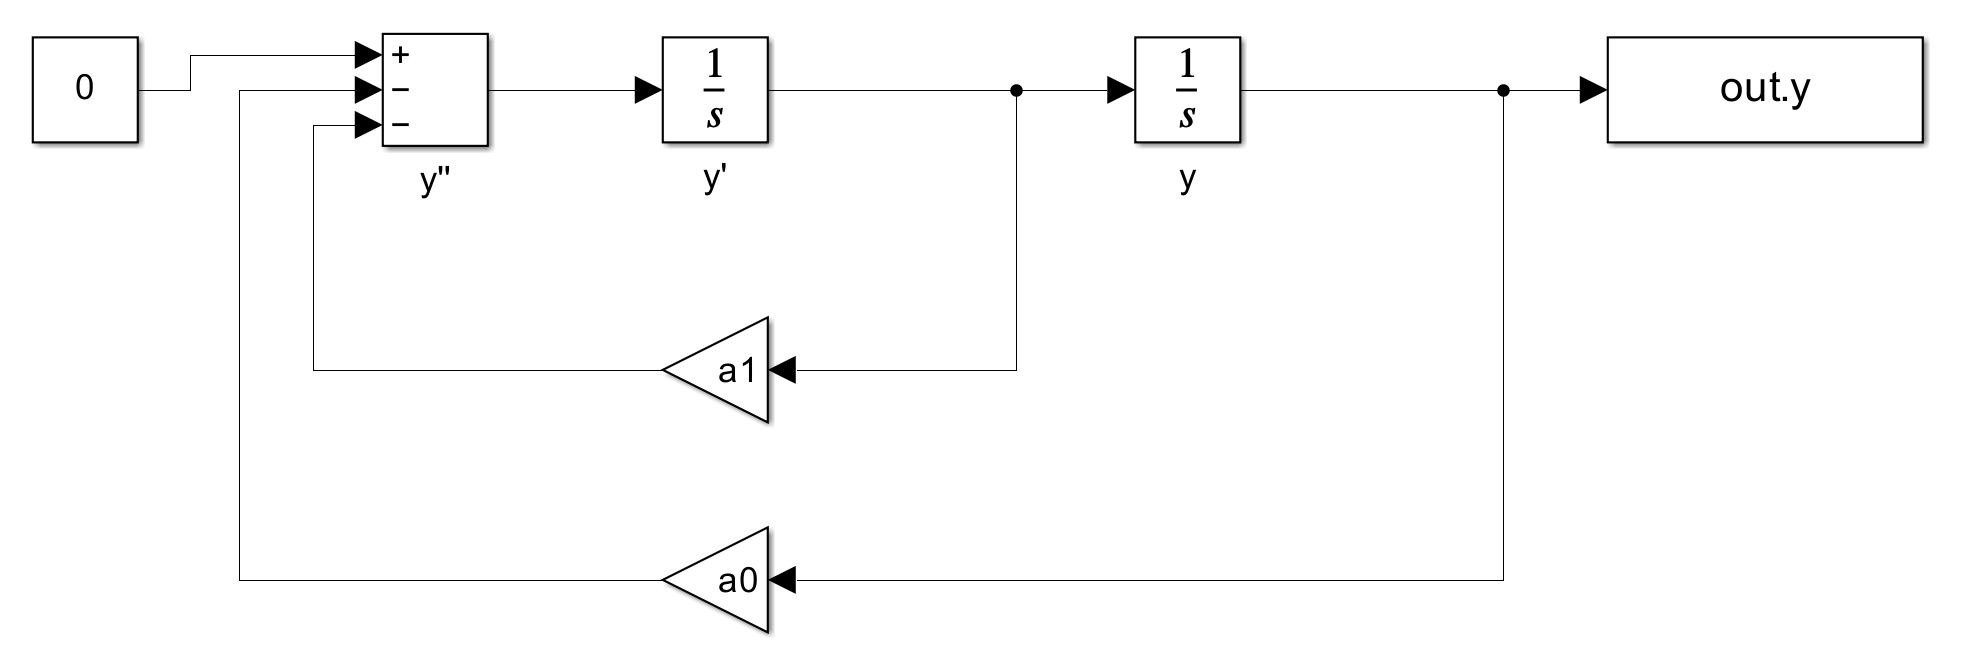
\includegraphics[width=1\textwidth, trim={0cm 0cm 0cm 0cm}]{../images/sim1.png}
    \caption{Схема разомкнутой системы в Simulink} 
\end{figure}
\begin{figure}[H]
    \centering
    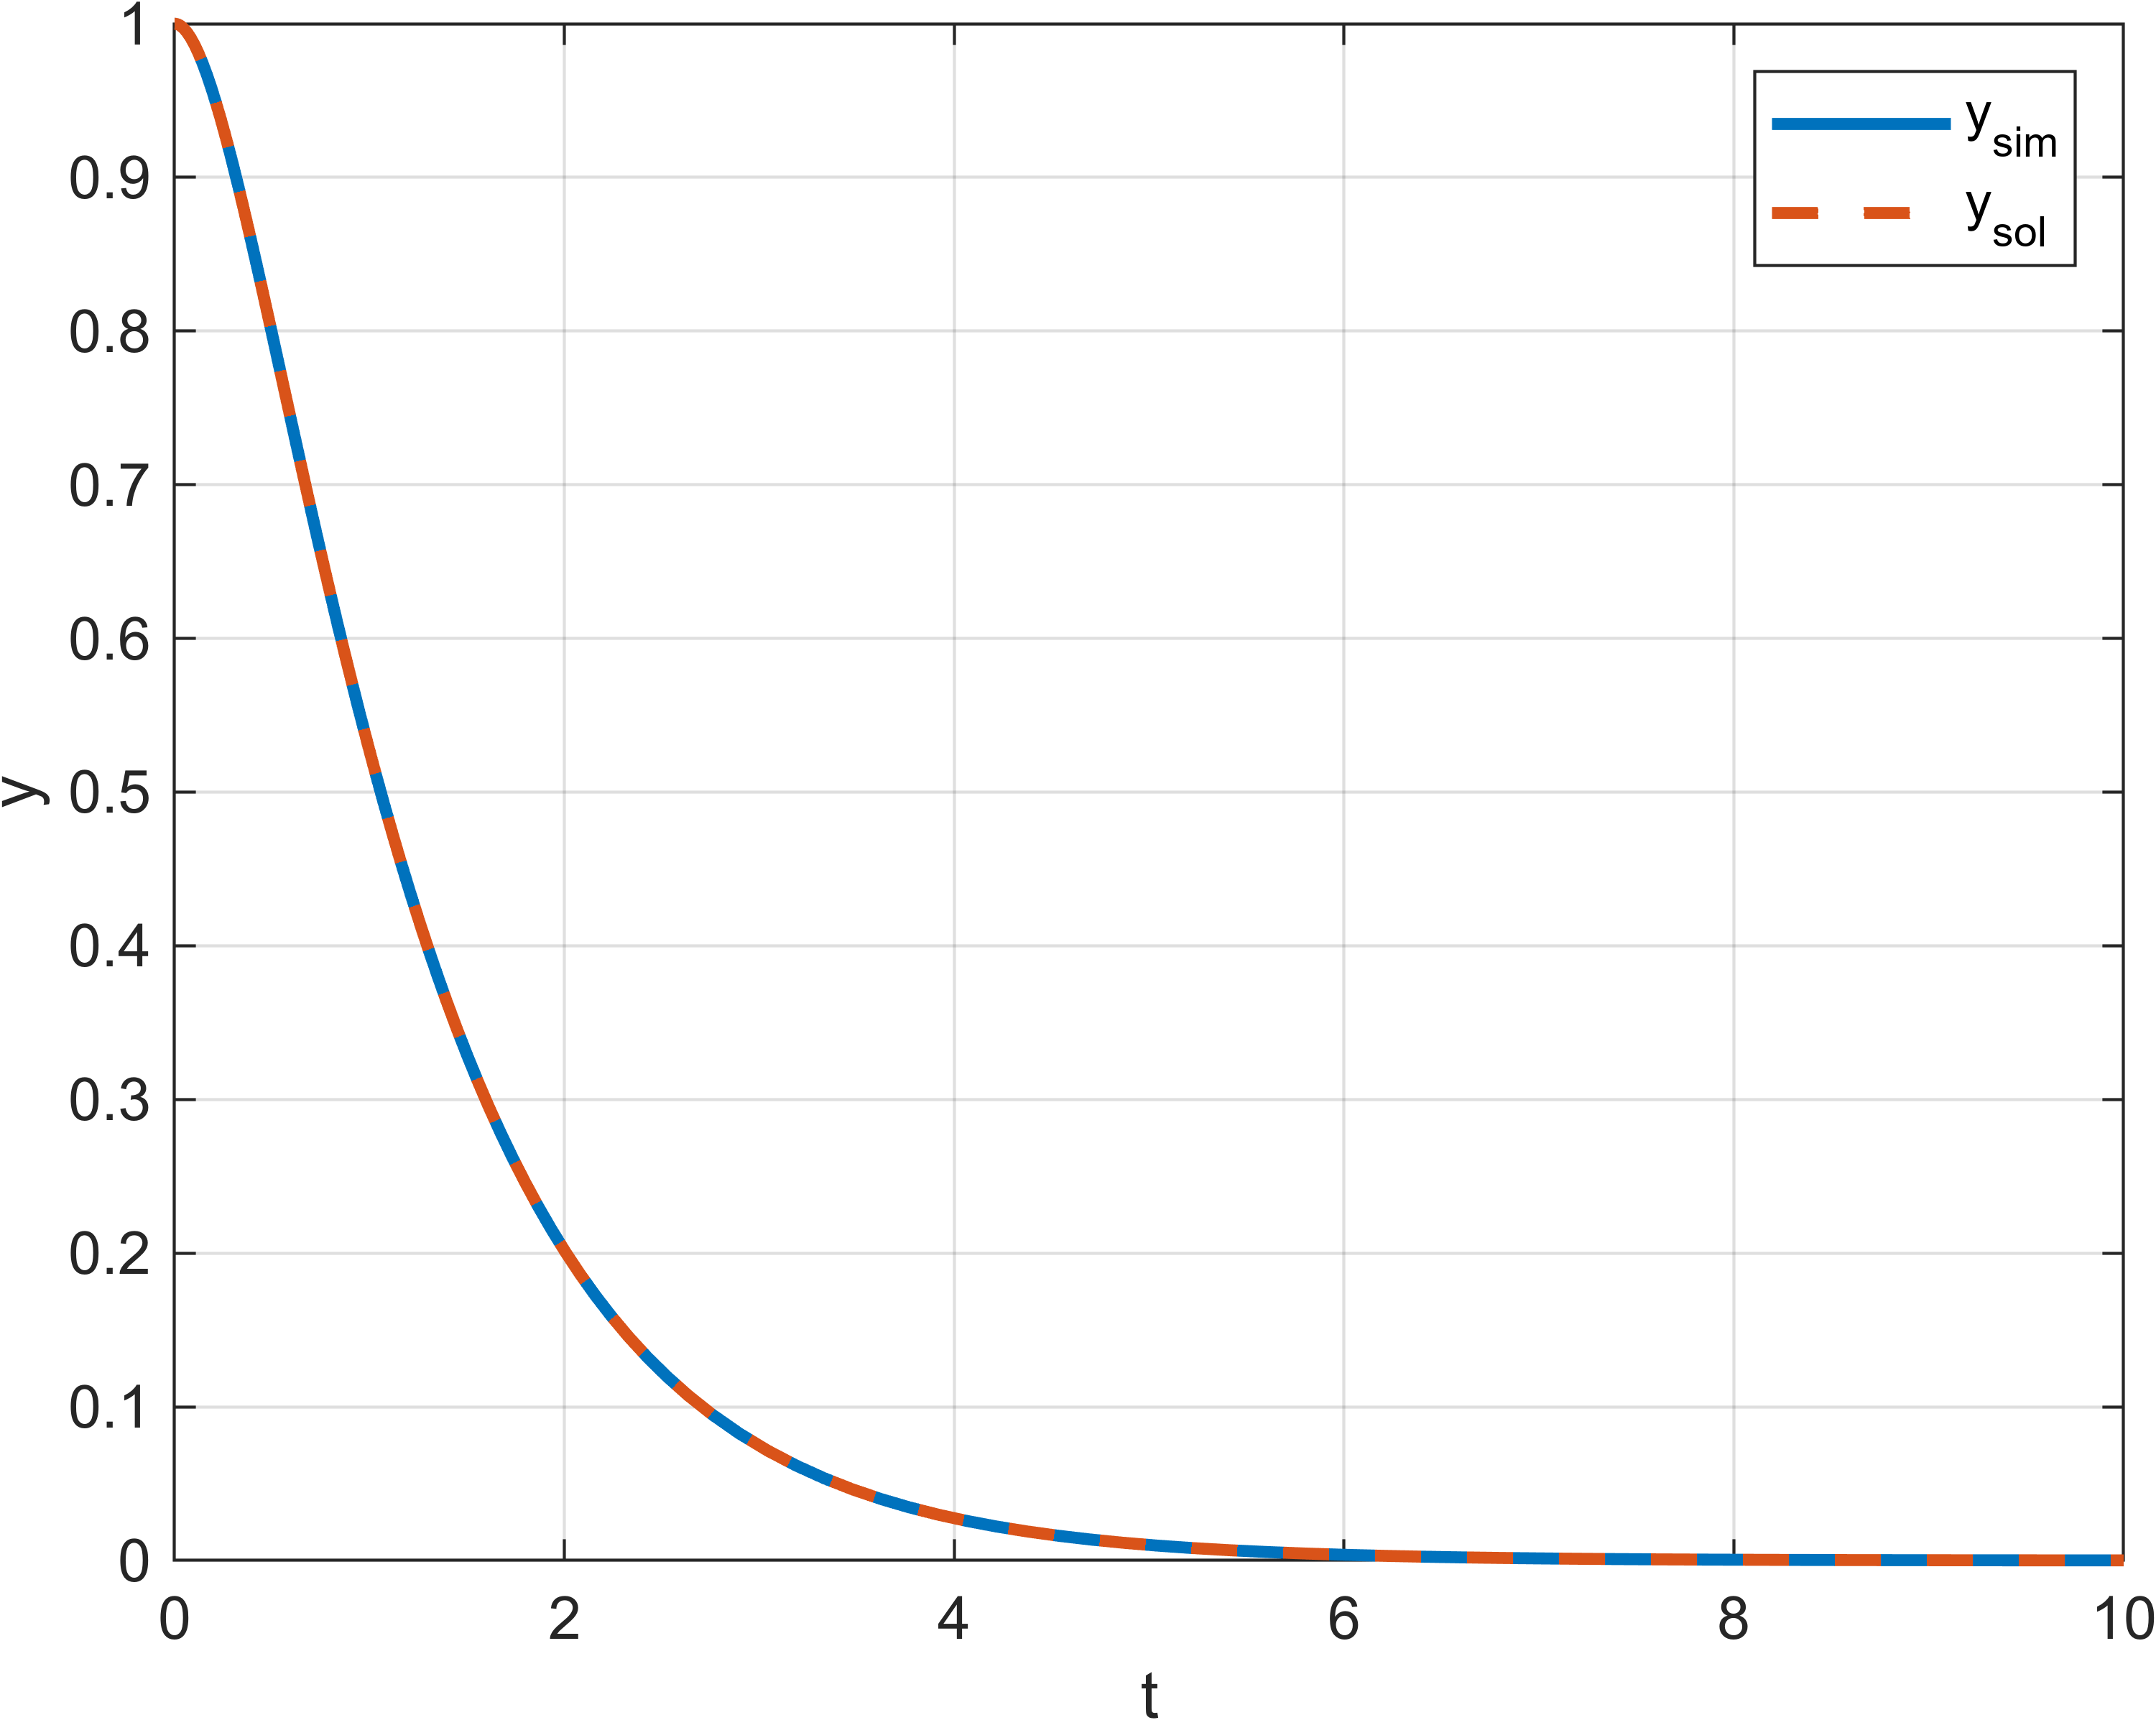
\includegraphics[width=1\textwidth, trim={0cm 0cm 0cm 0cm}]{../images/1_1.png}
    \caption{Сигнал разомкнутой системы $y_{\text{раз}}(t)$} 
\end{figure}

Рассмотрим регулятор вида:
\[
u = k_0y + k_1\dot{y}
\]

Построим структурную схему замкнутой системы, состоящей из объекта 
управления и регулятора, в режиме стабилизации:

\begin{figure}[H]
    \centering
    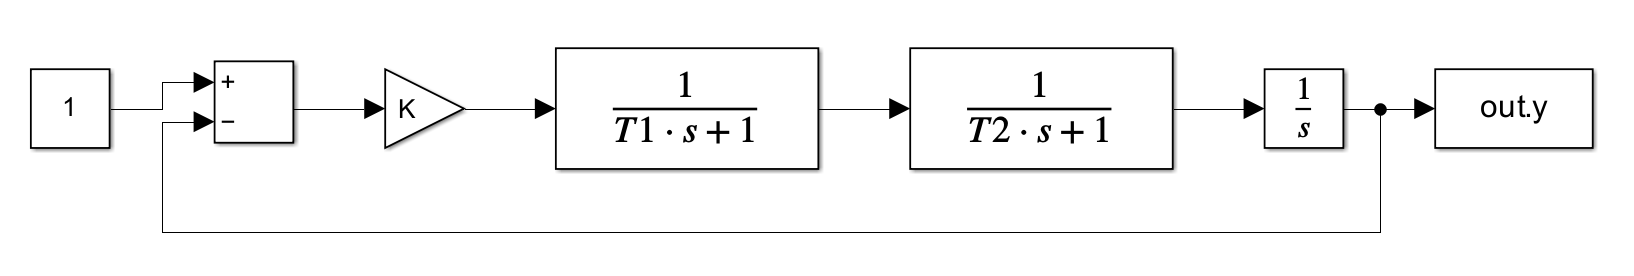
\includegraphics[width=1\textwidth, trim={0cm 0cm 0cm 0cm}]{../images/sim2.png}
    \caption{Схема замкнутой системы в Simulink}
\end{figure}

Найдем параметры $k_0$ и $k_1$, обеспечивающие асимптотически устойчивую замкнутую систему: 
\[
\ddot{y} - \dot{y} + y = k_0y + k_1\dot{y}
\]
\[
\ddot{y} + \dot{y}(-1 - k_1) + y(1 - k_0) = 0
\]
\[
\begin{cases}
    1 - k_0 > 0 \\
    -1 - k_1 > 0
\end{cases}
\]
\[
\begin{cases}
    k_0 < 1 \\
    k_1 < -1
\end{cases}
\]

Возьмем $k_0 = 1$, $k_1 = -3$ и проведем моделирование. А также сопоставим графики $y_{\text{раз}}(t)$ и $y_{\text{з}}(t)$:
\begin{figure}[H]
    \centering
    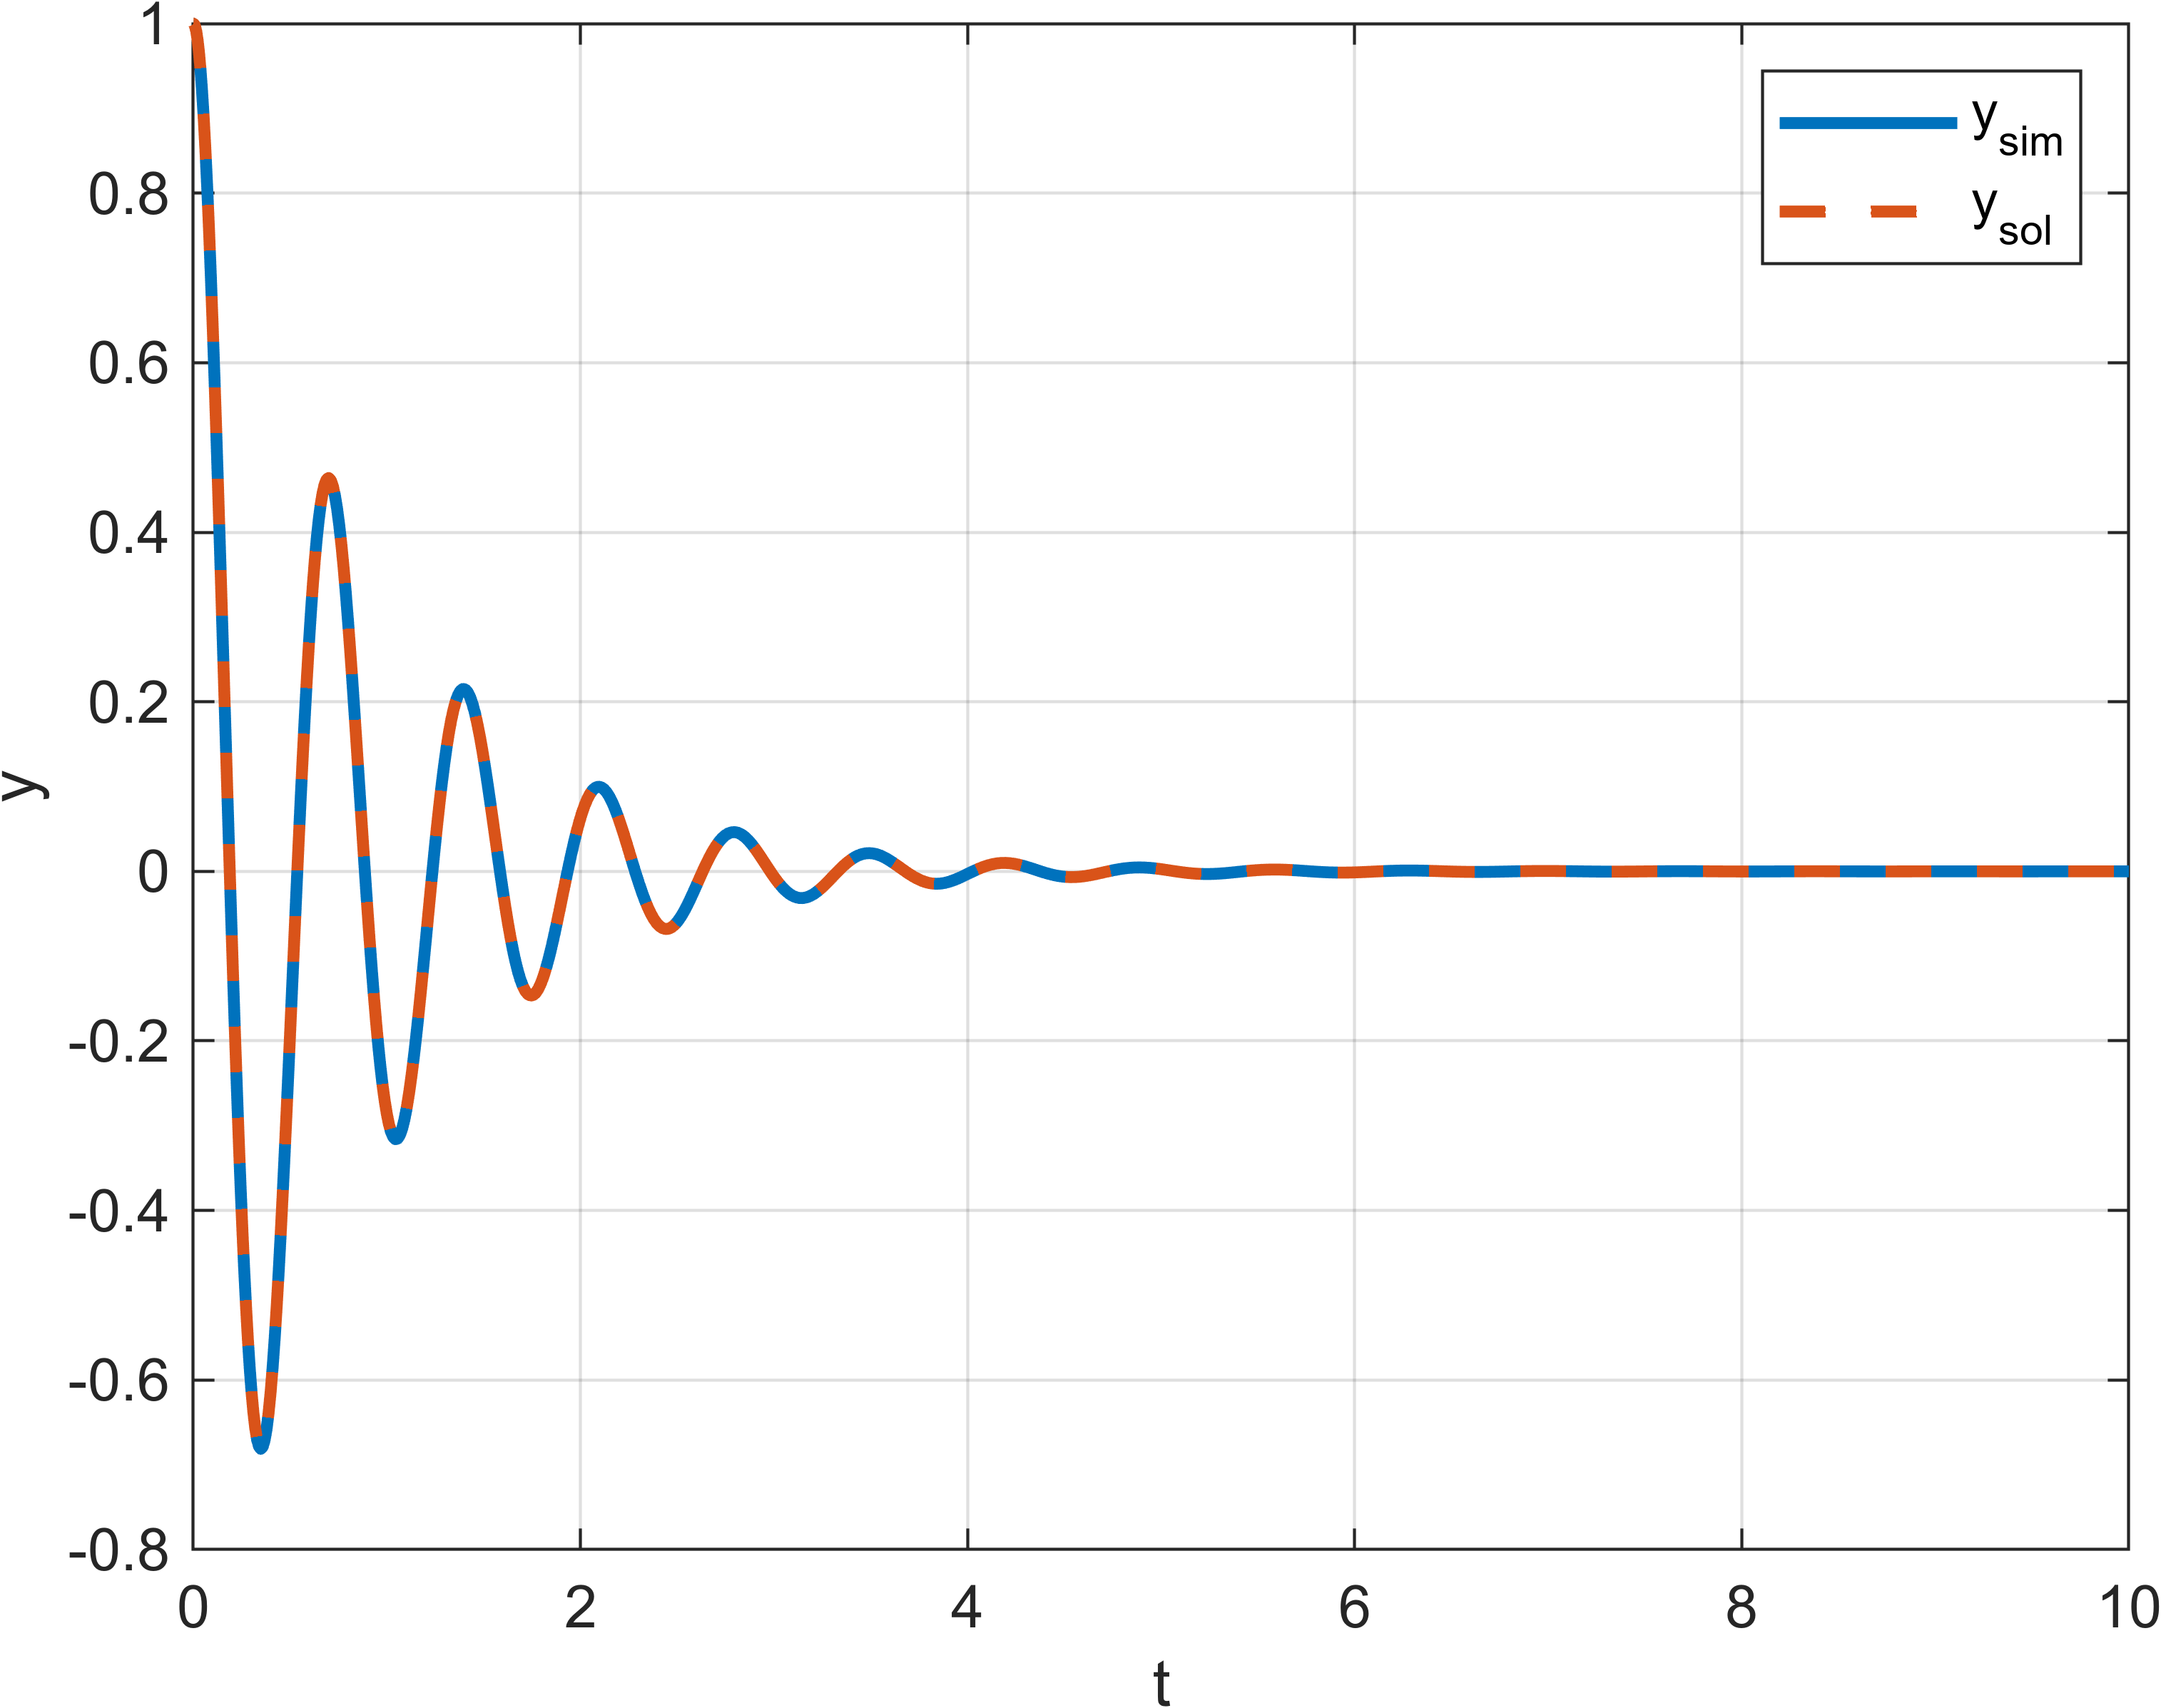
\includegraphics[width=0.75\textwidth, trim={0cm 0cm 0cm 0cm}]{../images/1_2.png}
    \caption{Сигнал замкнутой системы $y_{\text{з}}(t)$}
\end{figure}

\begin{figure}[H]
    \centering
    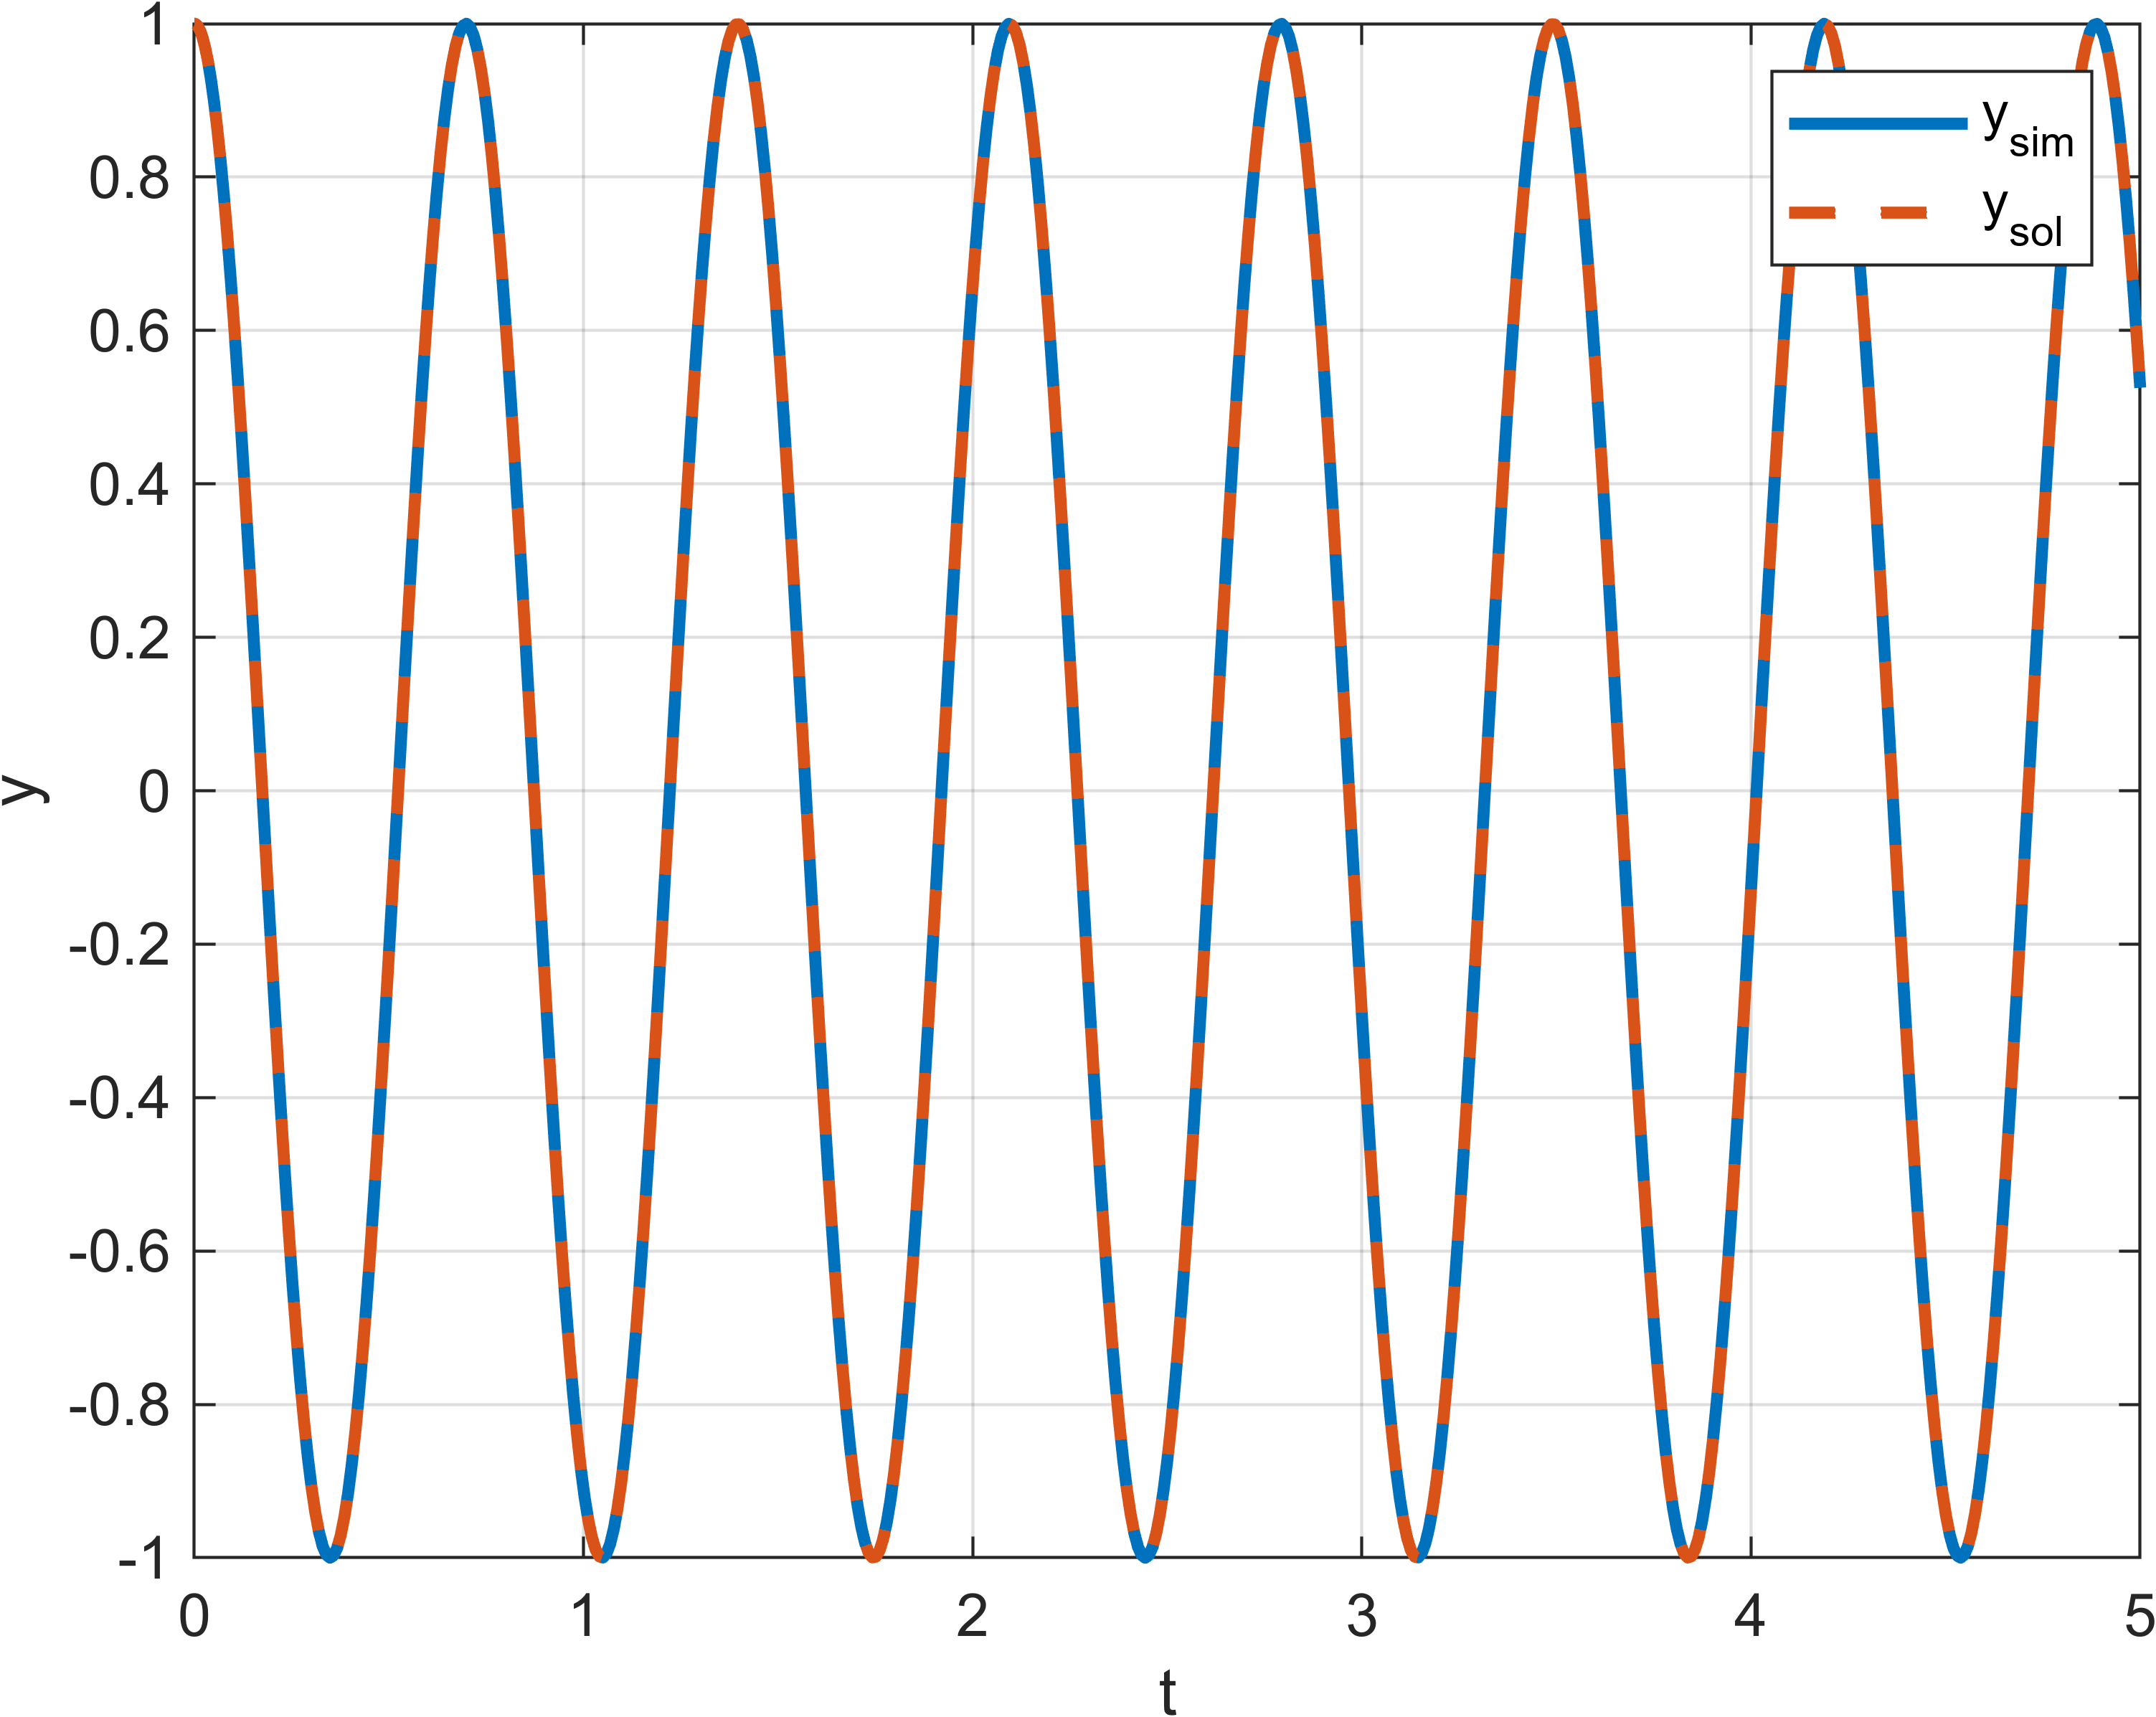
\includegraphics[width=0.75\textwidth, trim={0cm 0cm 0cm 0cm}]{../images/1_3.png}
    \caption{Сравнение сигналов $y_{\text{раз}}(t)$ и $y_{\text{з}}(t)$}
\end{figure}

Из графиков видно, что регулятор с идеальным дифференцирующим звеном
весьма хорошо обеспечивает стабилизацию системы.
\endinput 
\chapter{Объект 2. ДПТ 2.0}
Рассмотрим уравнения для двигателя постоянного тока независимого возбуждения:
\[
J\dot{\omega} = M, \quad M = k_m I, \quad I = \frac{U + \varepsilon_i}{R}, 
\quad \varepsilon = \varepsilon_i + \varepsilon_s, \quad \varepsilon_s = -L\dot I.
\]

где:
\begin{itemize}
    \item[] \( k_m \) — конструктивная постоянная по моменту
    \item[] \( L \) — индуктивность обмоток статора
    \item[] \( J \) — момент инерции ротора
    \item[] \( R \) — активное сопротивление обмоток ротора
    \item[] \( \varepsilon_i \) — ЭДС индукции
    \item[] \( \varepsilon_s \) — ЭДС самоиндукции
    \item[] \( \varepsilon \) — общая ЭДС
\end{itemize}

Со следующими параметрами:
\begin{itemize}
    \item[] \( k_m = 0.3348\, \text{Н} \cdot \text{м} / \text{А} \)
    \item[] \( k_e = 0.3348\, \text{В} \cdot \text{с}\)
    \item[] \( J = 0.0032\, \text{кг} \cdot \text{м}^2\)
    \item[] \( R = 4.7391\, \text{Ом}\)
    \item[] \( L =  1.1647\, \text{Гн} \)
\end{itemize}

Передаточная функция ДПТ имеет вид:
\[
    W(s) = \frac{\omega}{U} = \frac{\frac{1}{k_e}}{\frac{LJ}{k_e k_m}s^2 + \frac{JR}{k_e k_m}s + 1}
\]

Что является колебательным звеном, имеющим передаточную функцию вида:
\[
    W(s) = \frac{K}{T^2 s^2 + 2 \xi T s + 1}
\]

где:
\begin{itemize}
    \item[] \( K \) — коэффициент усиления
    \item[] \( T \) — постоянная времени
    \item[] \( \xi \) — коэффициент затухания
\end{itemize}

Соответственно, коэффициенты $K$, $T$ и \( \xi \) равны:

\[
    K = k_e^{-1} = 2.9869, \quad T = \sqrt{\frac{LJ}{k_e k_m}} = 0.1823, \quad \xi = \frac{R}{2} \sqrt{\frac{J}{Lk_e k_m}} = 0.037
\]

\section{Временные характеристики}

Переходная характеристика для колебательного звена имеет вид:
\[
h(t) = K \left( 1 - \frac{1}{\sqrt{1 - \xi^2}} e^{-\alpha t} \sin(\omega_0 t + \varphi) \right),
\]
\[
\omega_0 = \frac{\sqrt{1 - \xi^2}}{T}, \quad \alpha = \frac{\xi}{T}, \quad \varphi = \arctan\left(\frac{\sqrt{1 - \xi^2}}{\xi}\right)
\]

где:
\begin{itemize}
    \item[] \( \omega_0 \) — частота собственных колебаний
    \item[] \( \alpha \) — коэффициент затухания
    \item[] \( \varphi \) — начальная фаза
\end{itemize}

Весовая характеристика для колебательного звена имеет вид:
\[
    w(t) = K \left(\omega_0 + \frac{\alpha^2}{\omega_0}\right) \sin(\omega_0 t) e^{-\alpha t}.
\]

\begin{figure}[H]
    \centering
    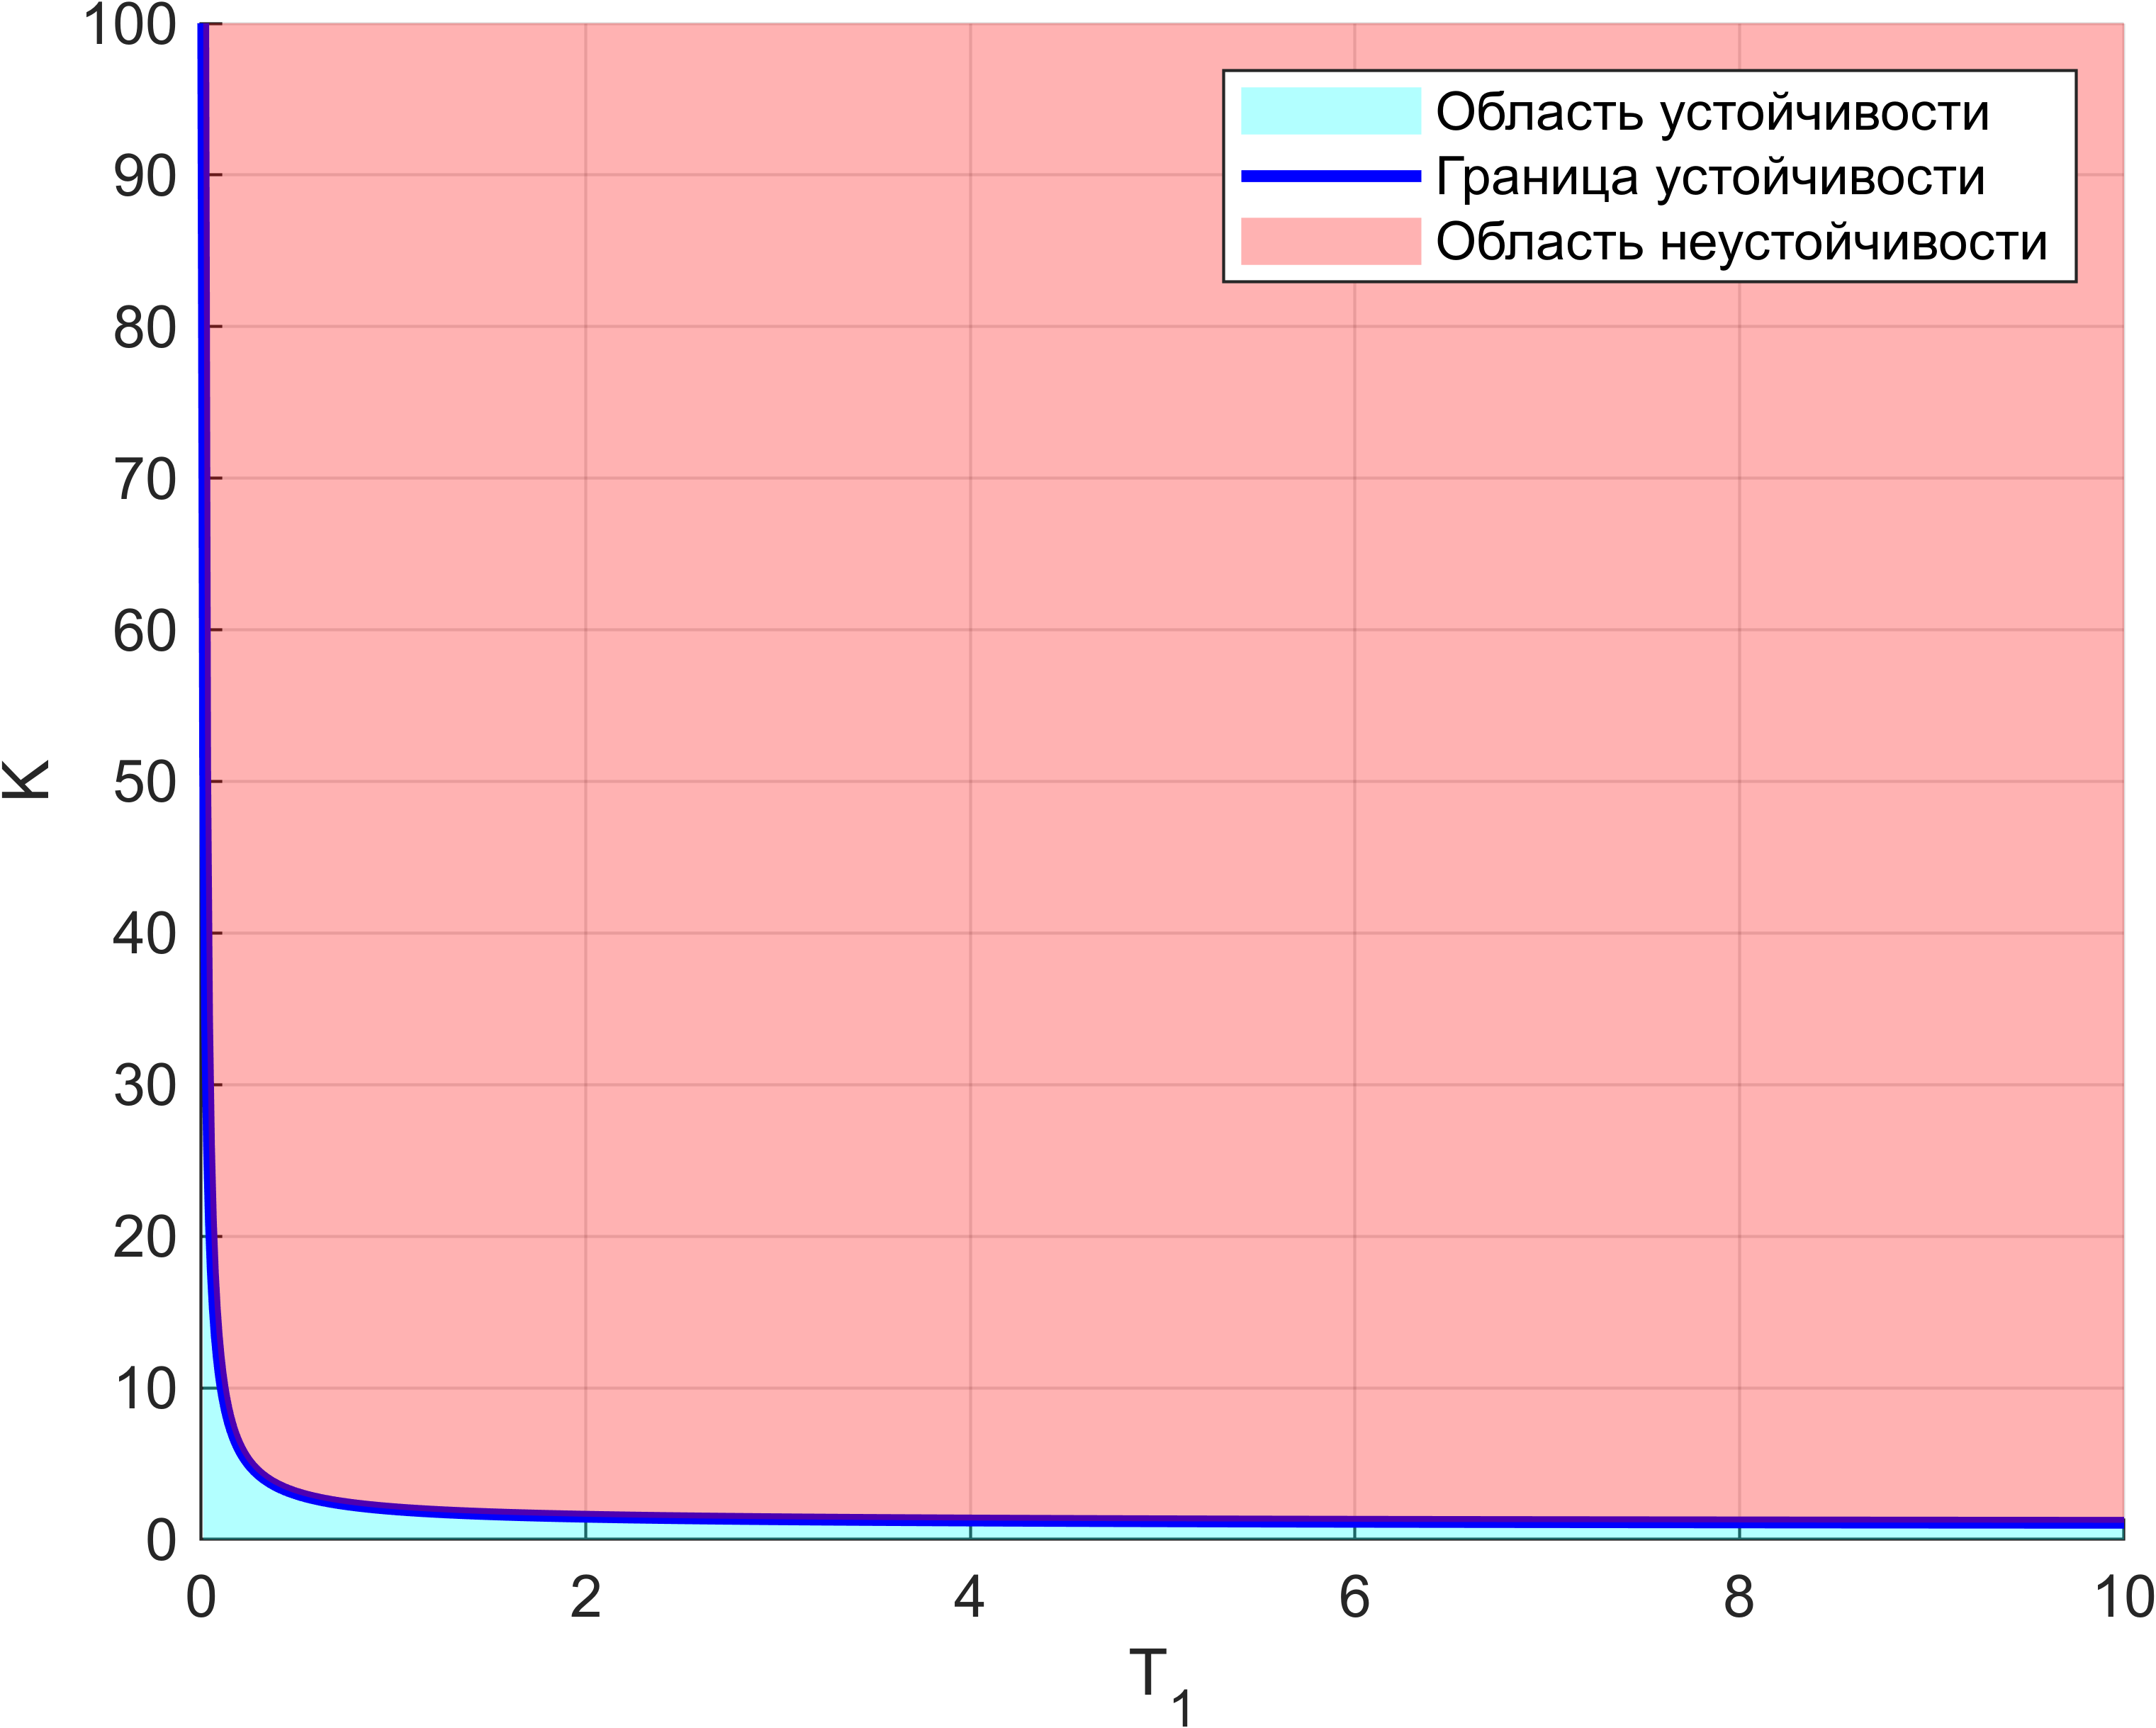
\includegraphics[width=0.75\textwidth, trim={0cm 0cm 0cm 0cm}]{../images/2_1.png}
    \caption{Переходная характеристика полной модели ДПТ} 
\end{figure}

\begin{figure}[H]
    \centering
    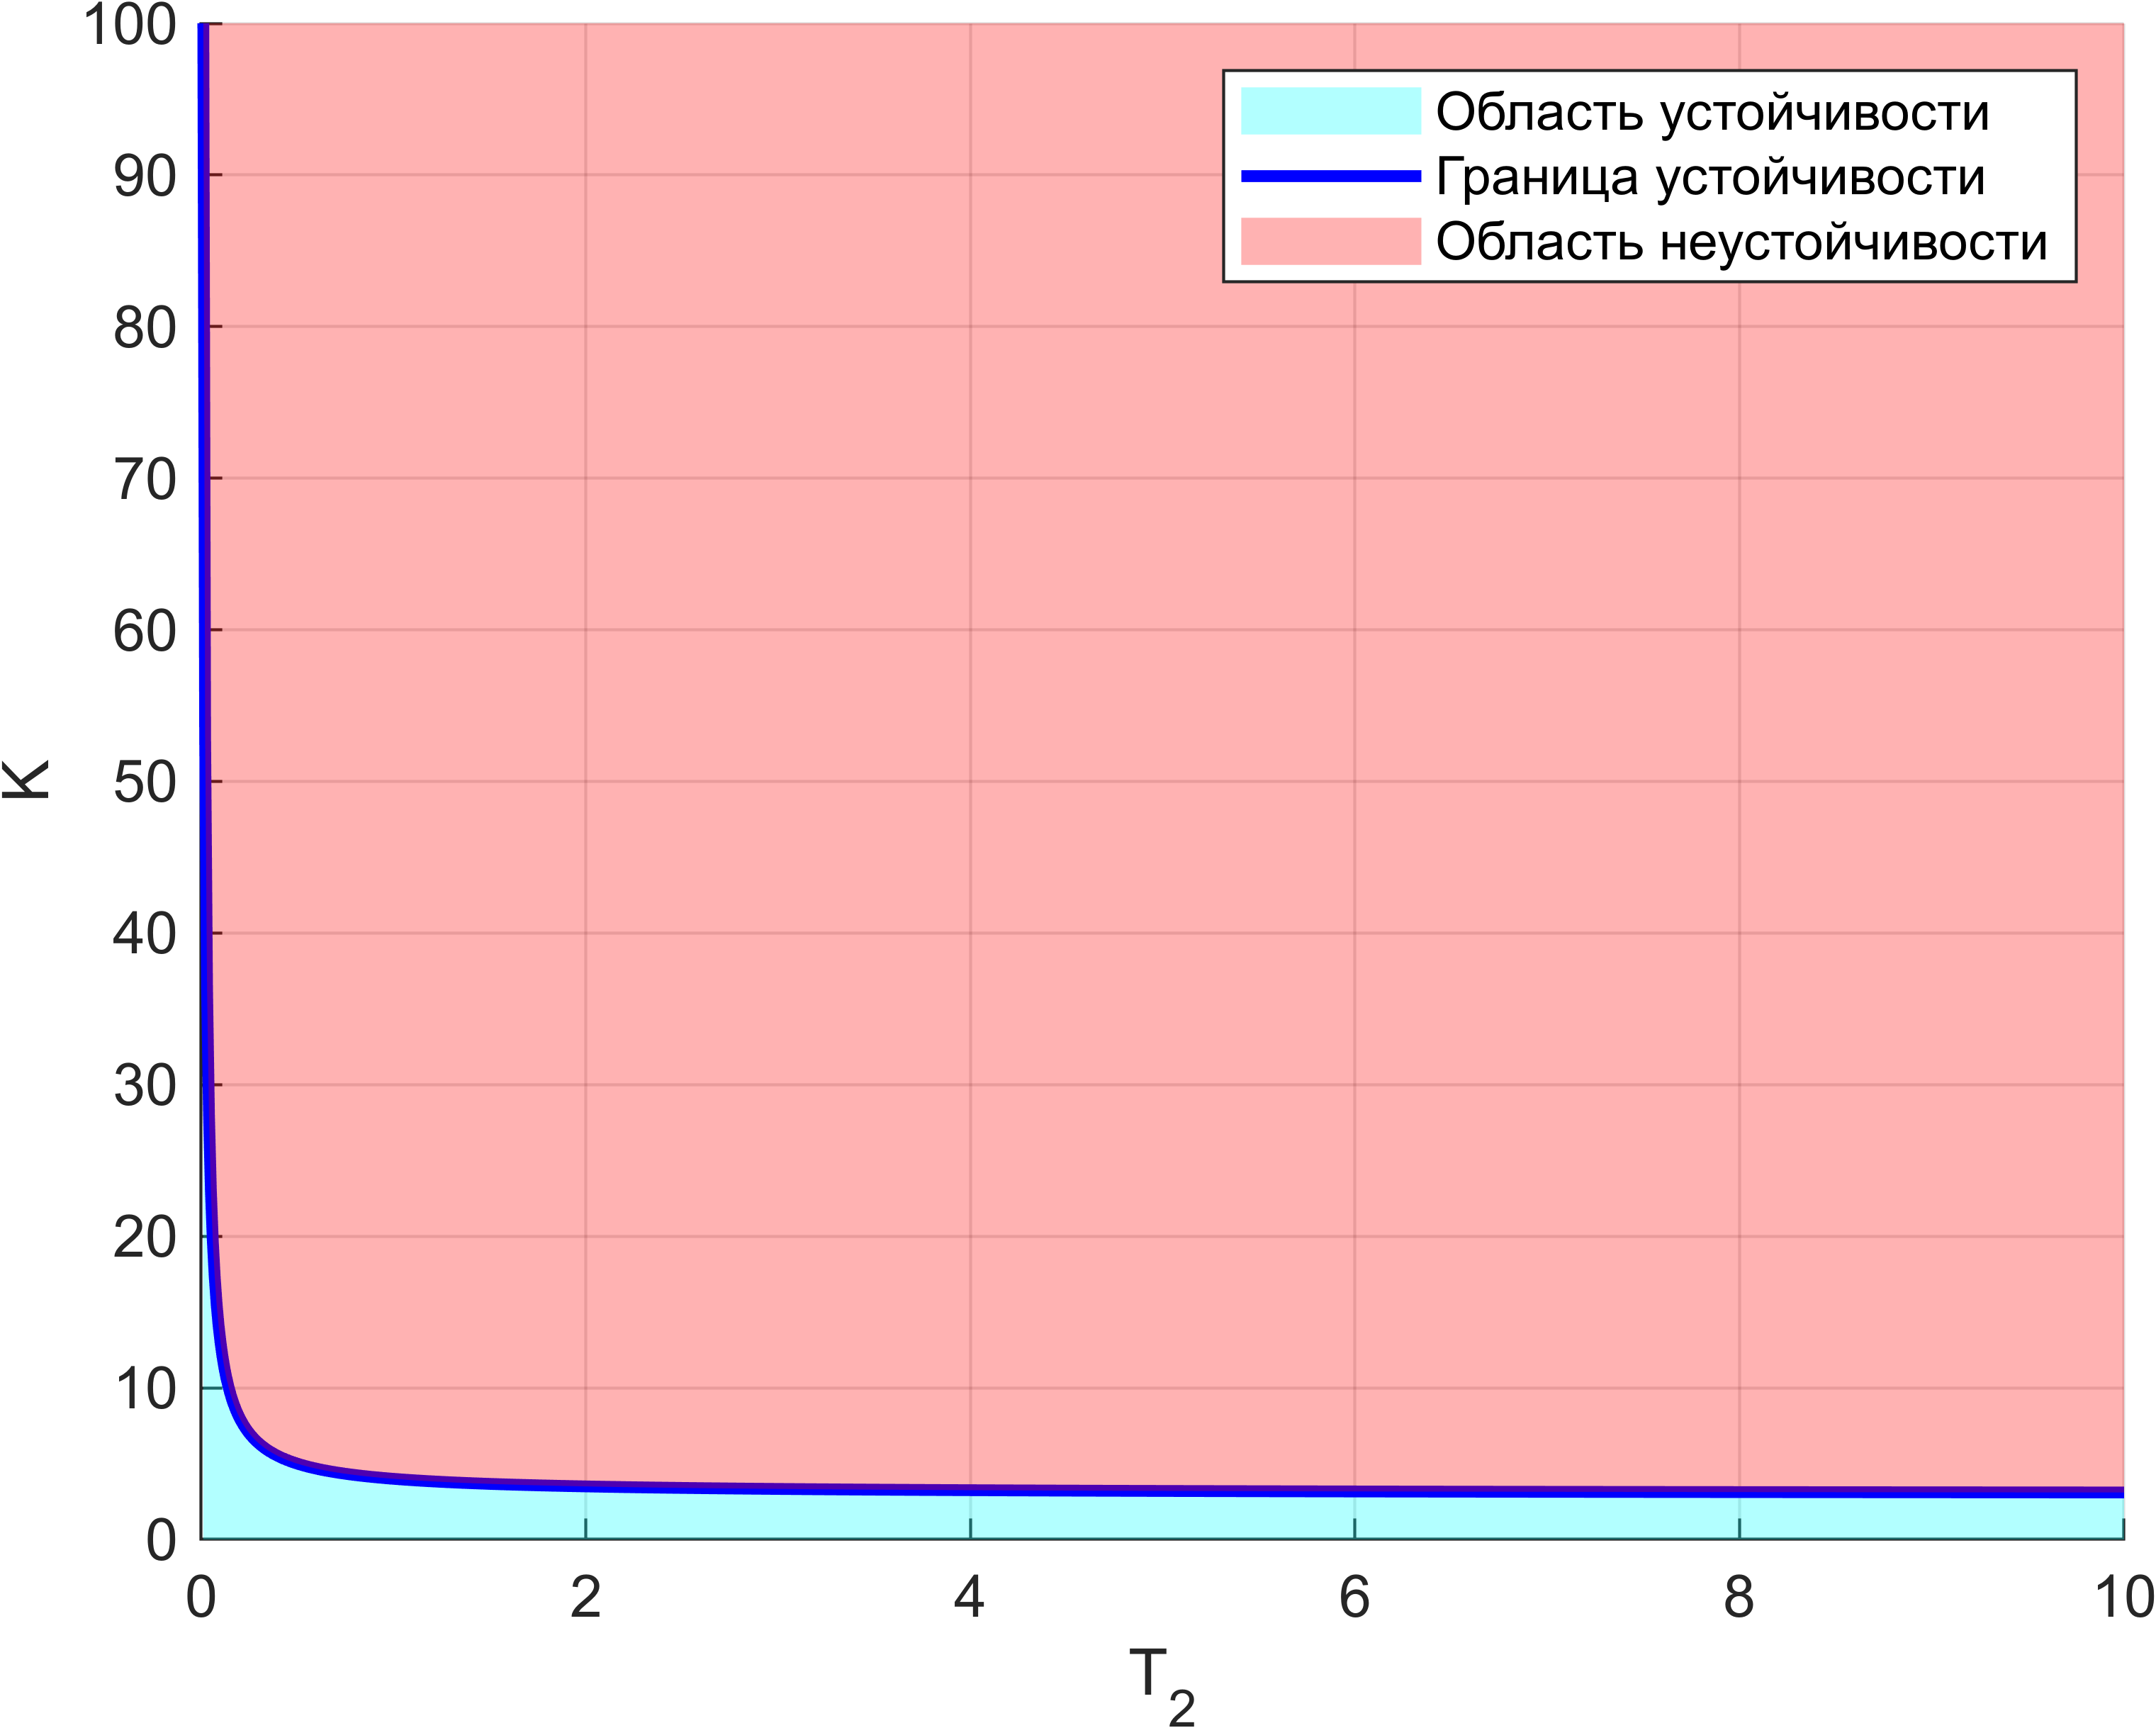
\includegraphics[width=0.75\textwidth, trim={0cm 0cm 0cm 0cm}]{../images/2_2.png}
    \caption{Весовая характеристика полной модели ДПТ}
\end{figure}

\section{Частотные характеристики}

Амплитудно-частотная характеристика для колебательного звена имеет вид:

\[
    A(\omega) = \frac{K}{\sqrt{(1 - \omega^2 T^2)^2 + (2 \xi \omega T)^2}}
\]

Логарифмическая амплитудно-частотная характеристика:
\[
    L(\omega) = 20 \lg(K) - 10 \lg\left((1 - \omega^2 T^2)^2 + 4 \omega^2 \xi^2 T^2\right)
\]

Фазо-частотная характеристика для колебательного звена имеет вид:
\[
    \varphi(\omega) = -a\pi - \arctan\left(\frac{2 \xi \omega T}{1 - \omega^2 T^2}\right), \quad 
    a = 
    \begin{cases} 
    0, & \omega < T^{-1} \\ 
    1, & \omega > T^{-1} 
    \end{cases}
\]

\begin{figure}[H]
    \centering
    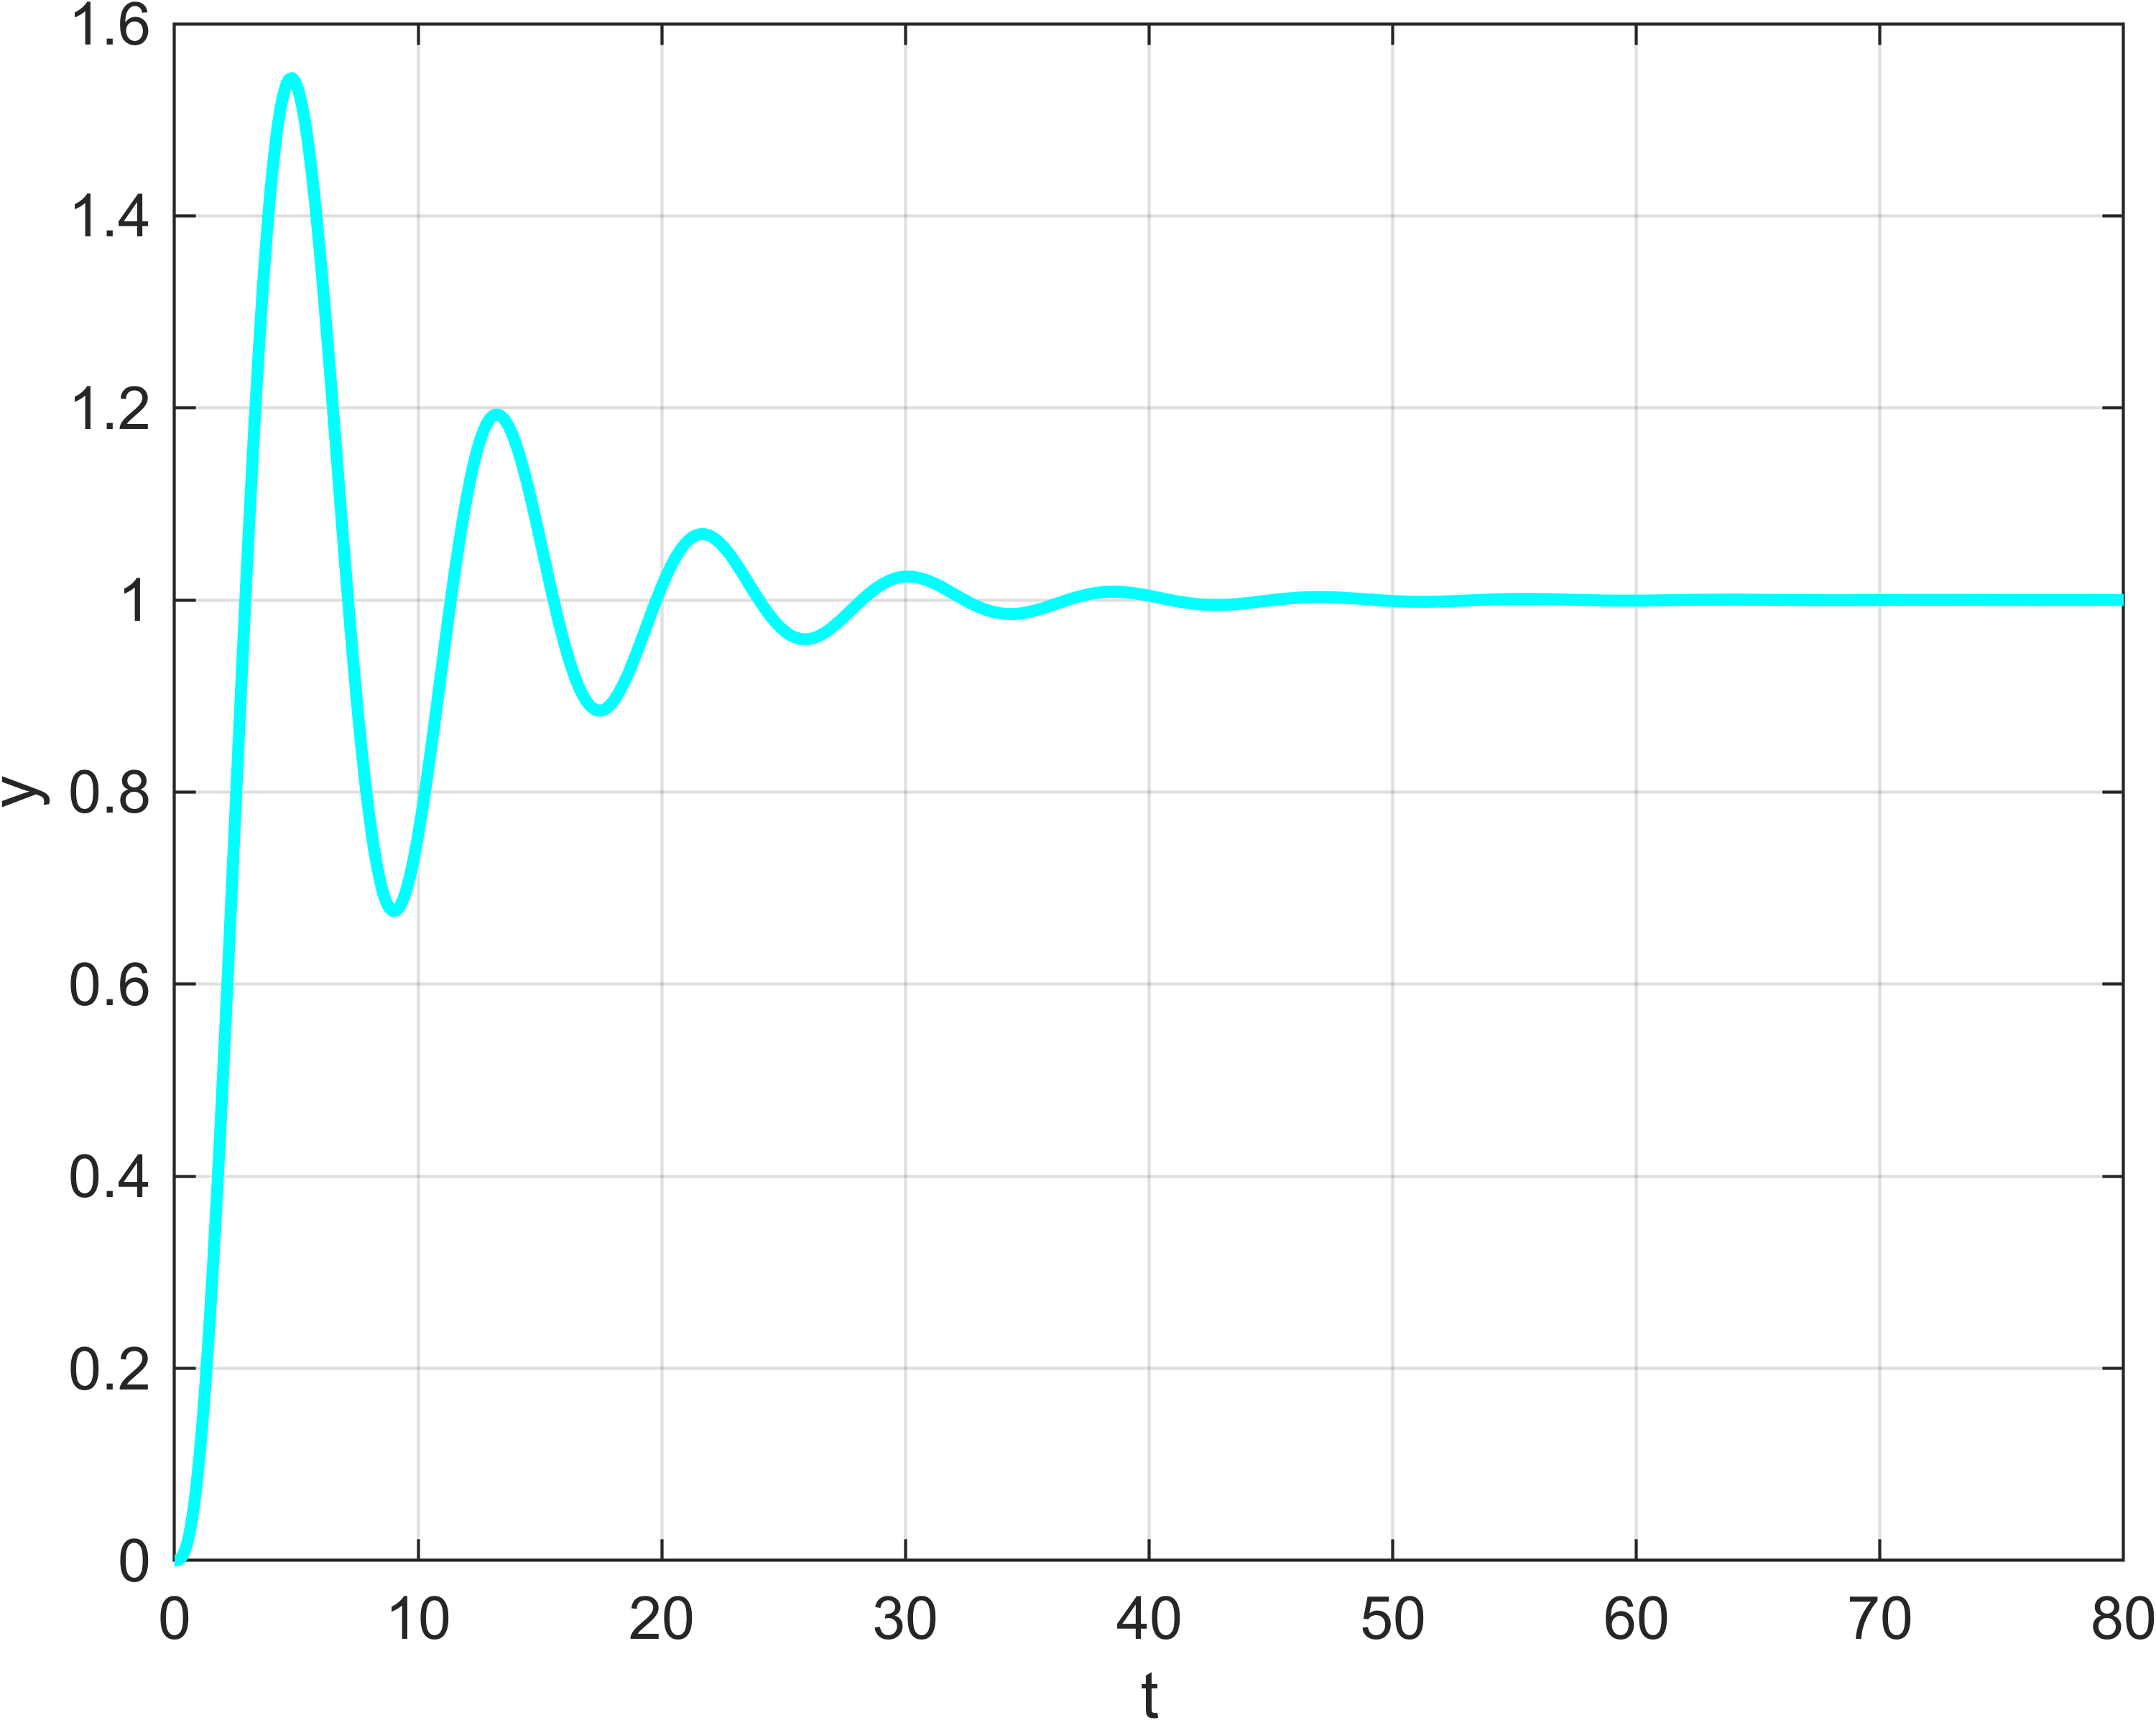
\includegraphics[width=0.75\textwidth, trim={0cm 0cm 0cm 0cm}]{../images/2_3.png}
    \caption{Амплитудно-частотная характеристика полной модели ДПТ}
\end{figure}

\begin{figure}[H]
    \centering
    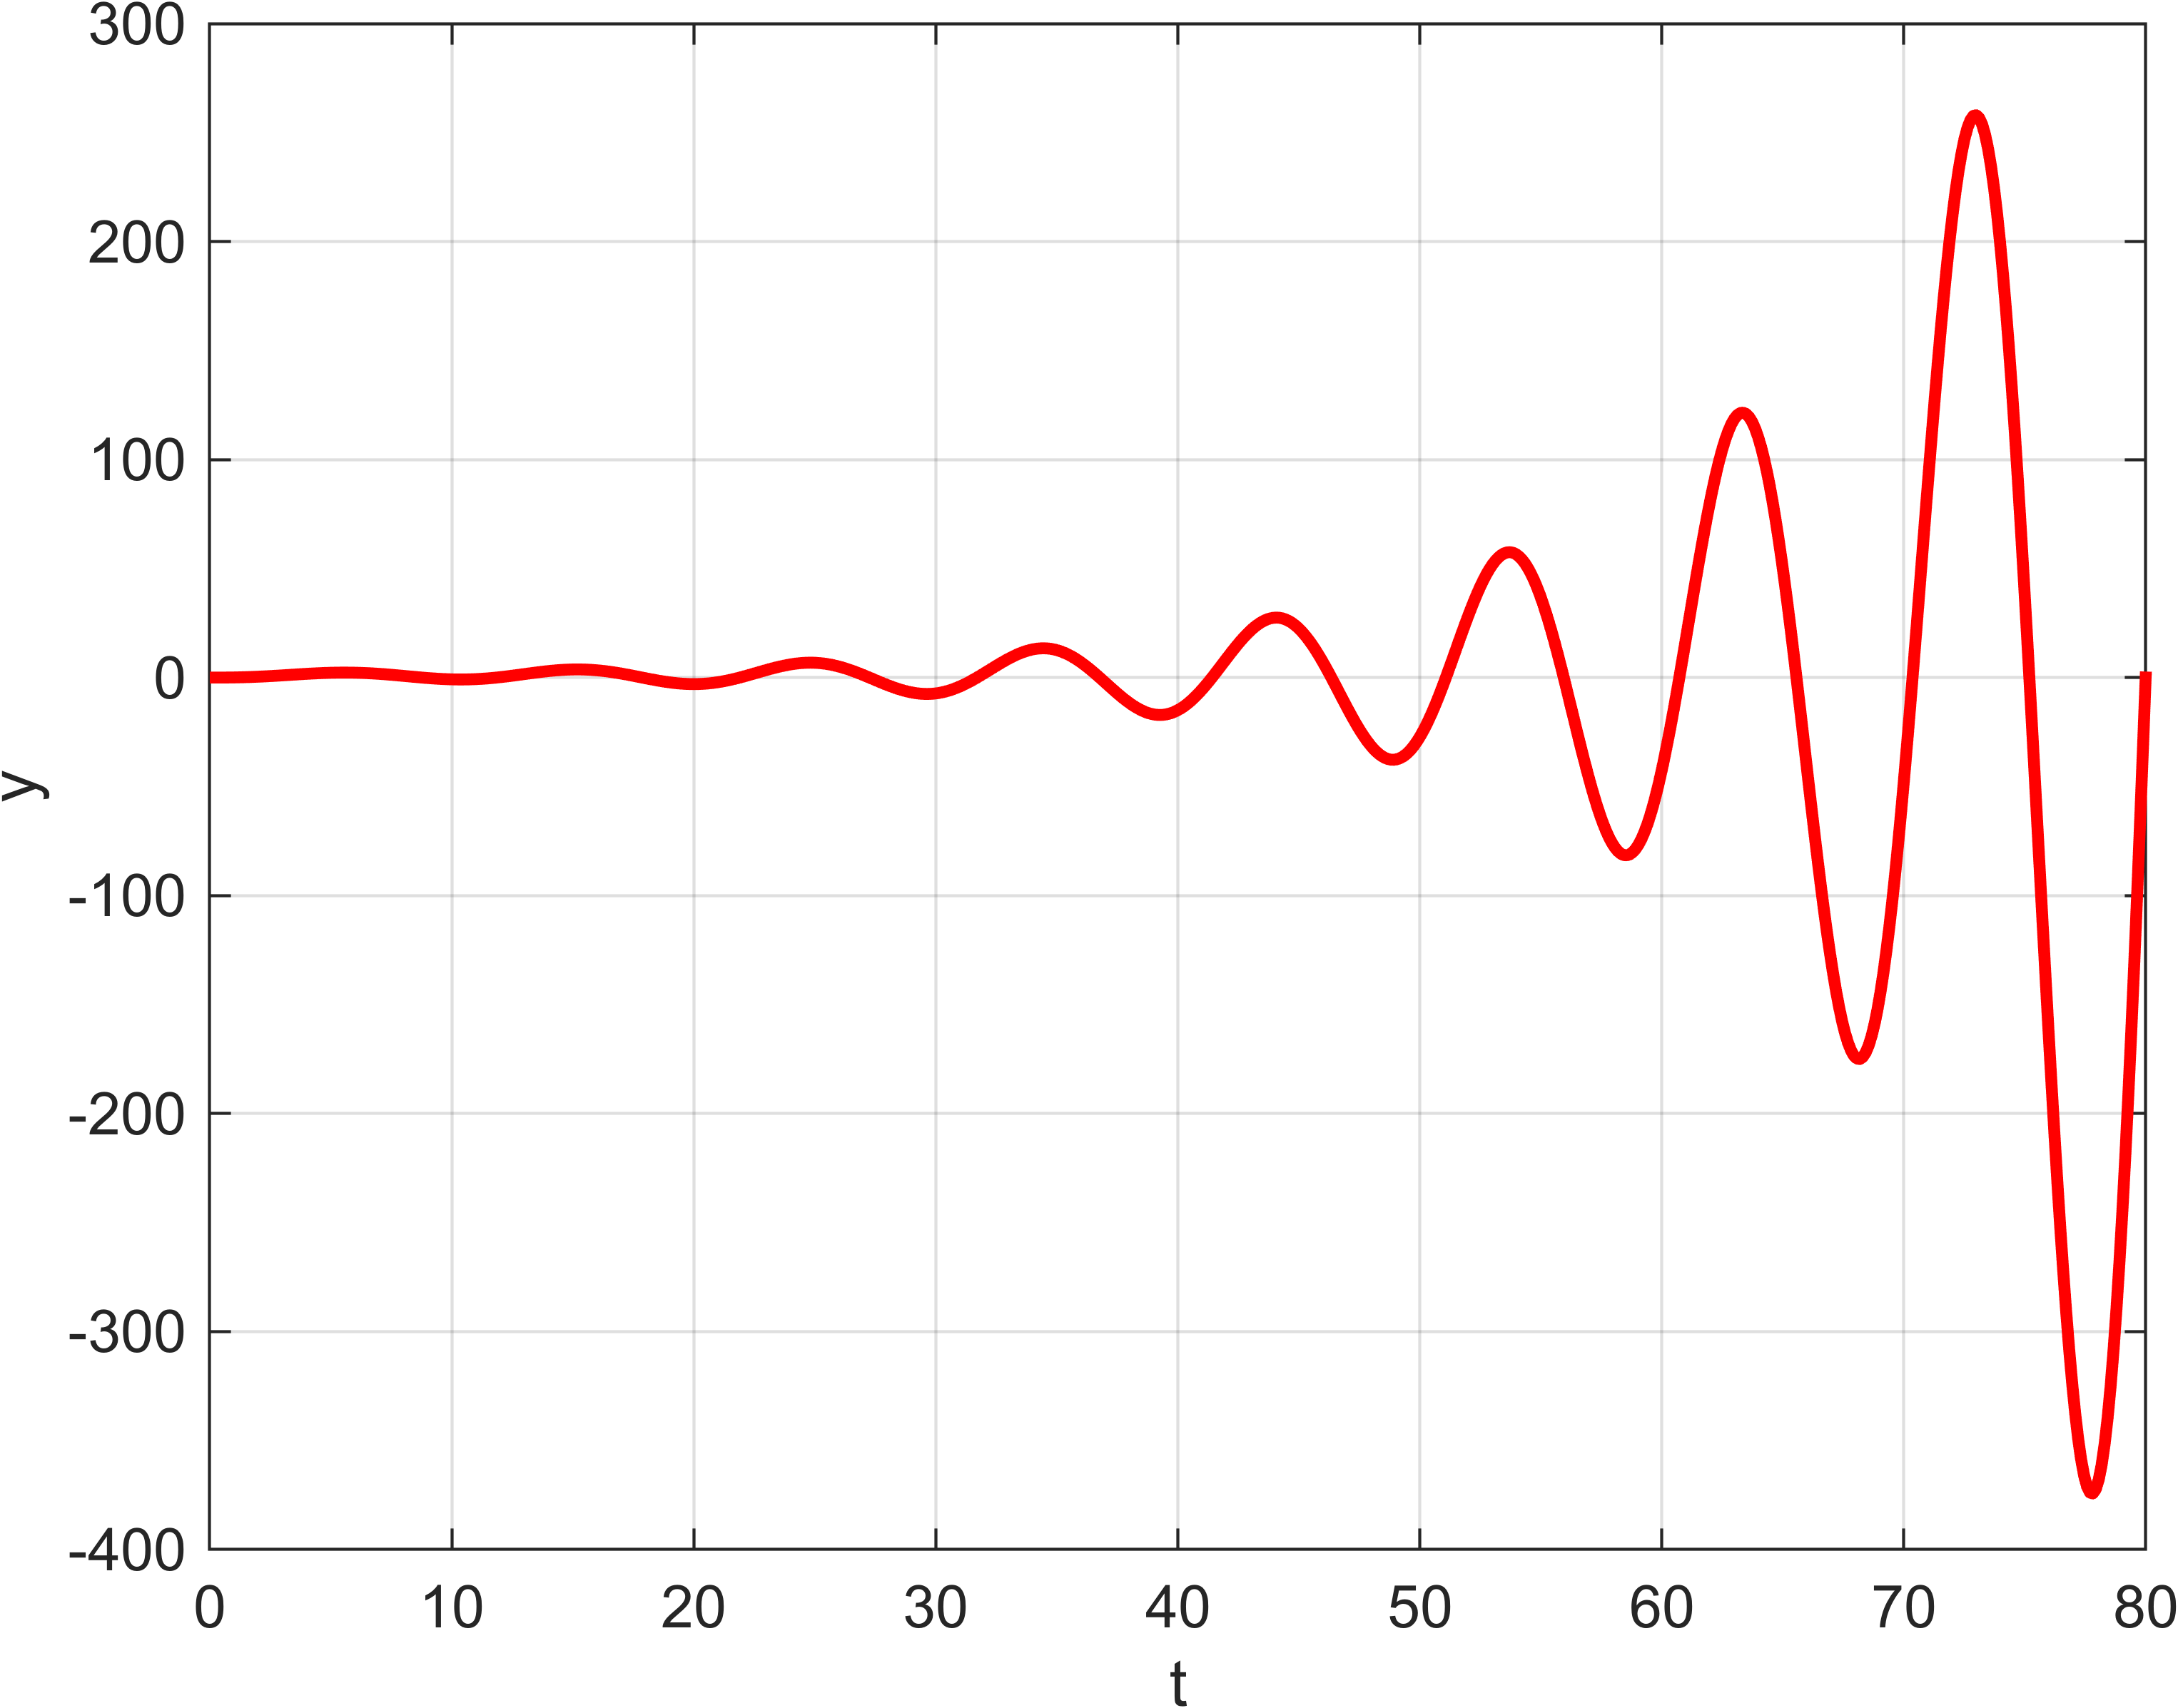
\includegraphics[width=0.75\textwidth, trim={0cm 0cm 0cm 0cm}]{../images/2_4.png}
    \caption{Фазо-частотная характеристика полной модели ДПТ}
\end{figure}

\begin{figure}[H]
    \centering
    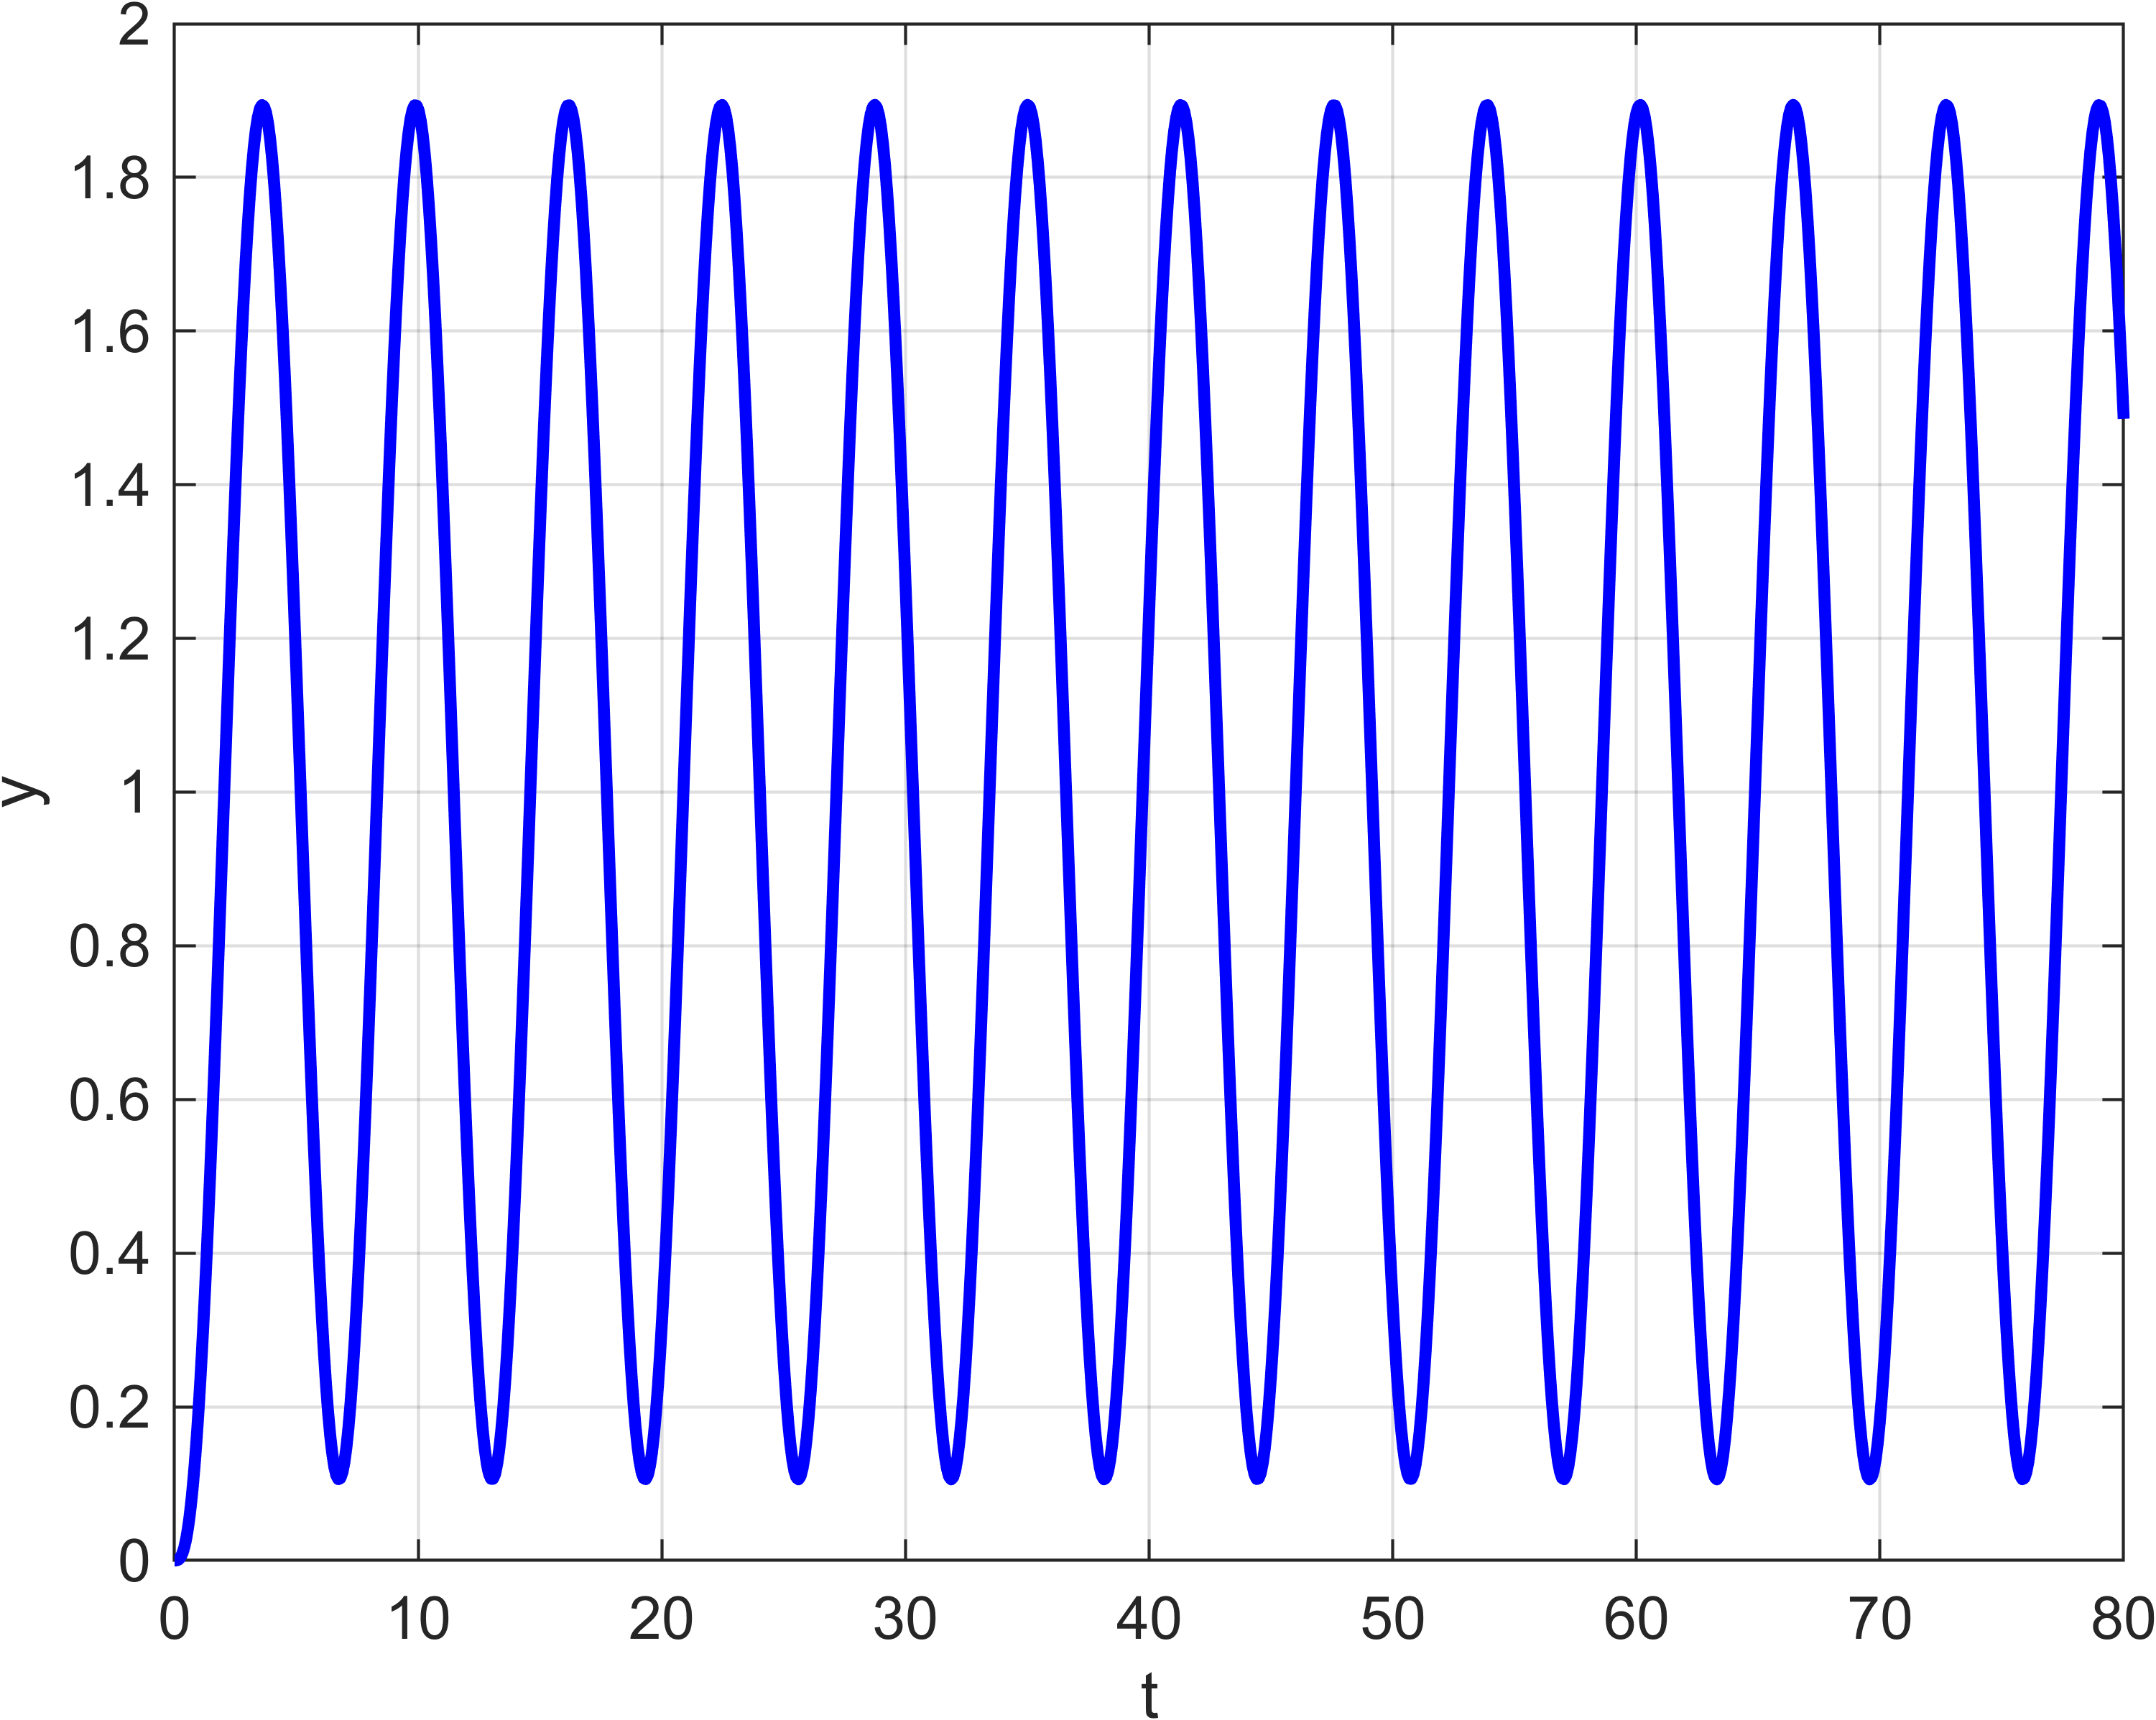
\includegraphics[width=0.75\textwidth, trim={0cm 0cm 0cm 0cm}]{../images/2_5.png}
    \caption{Логарифмическая амплитудно-фазо-частотная характеристика полной модели ДПТ}
\end{figure}

\endinput
\chapter{}

\endinput
% \chapter{Объект 4. Пружинка}
Рассмотрим уравнения пружинного маятника:
\[
    F_{\text{упр}} = -k x, \quad F = m \ddot{x}
\]

где:
\begin{itemize}
    \item[] \( k \) — коэффициент жесткости пружины
    \item[] \( m \) — масса груза
\end{itemize}

Со следующими параметрами:
\begin{itemize}
    \item[] \( k = 20\, \text{Н} / \text{м} \)
    \item[] \( m = 81\, \text{кг} \)
\end{itemize}

Запишем общее уравнение движения через некоторую силу \( F_{ext} \), 
направленную соосно движению маятника:
\[
    m \ddot{x} + k x = F_{ext}
\]

Передаточная функция пружинного маятника имеет вид:
\[
    W(s) = \frac{x}{F_{ext}} = \frac{\frac{1}{k}}{\frac{m}{k}s^2 + 1}
\]

Что является консервативным звеном, имеющим передаточную функцию вида:
\[
    W(s) = \frac{K}{T^2 s^2 + 1}
\]

Соответственно, коэффициенты \( K \) и \( T \) равны:
\[
    K = \frac{1}{k} = 0.0123, \quad T = \sqrt{\frac{m}{k}} = 0.4969
\]

\section{Временные характеристики}

Переходная характеристика для консервативного звена имеет вид:
\[
    h(t) = K \left( 1 - cos(\omega_0 t) \right)
\]

Весовая характеристика для консервативного звена имеет вид:
\[
    w(t) = K \omega_0 \sin(\omega_0 t)
\]

\begin{figure}[H]
    \centering
    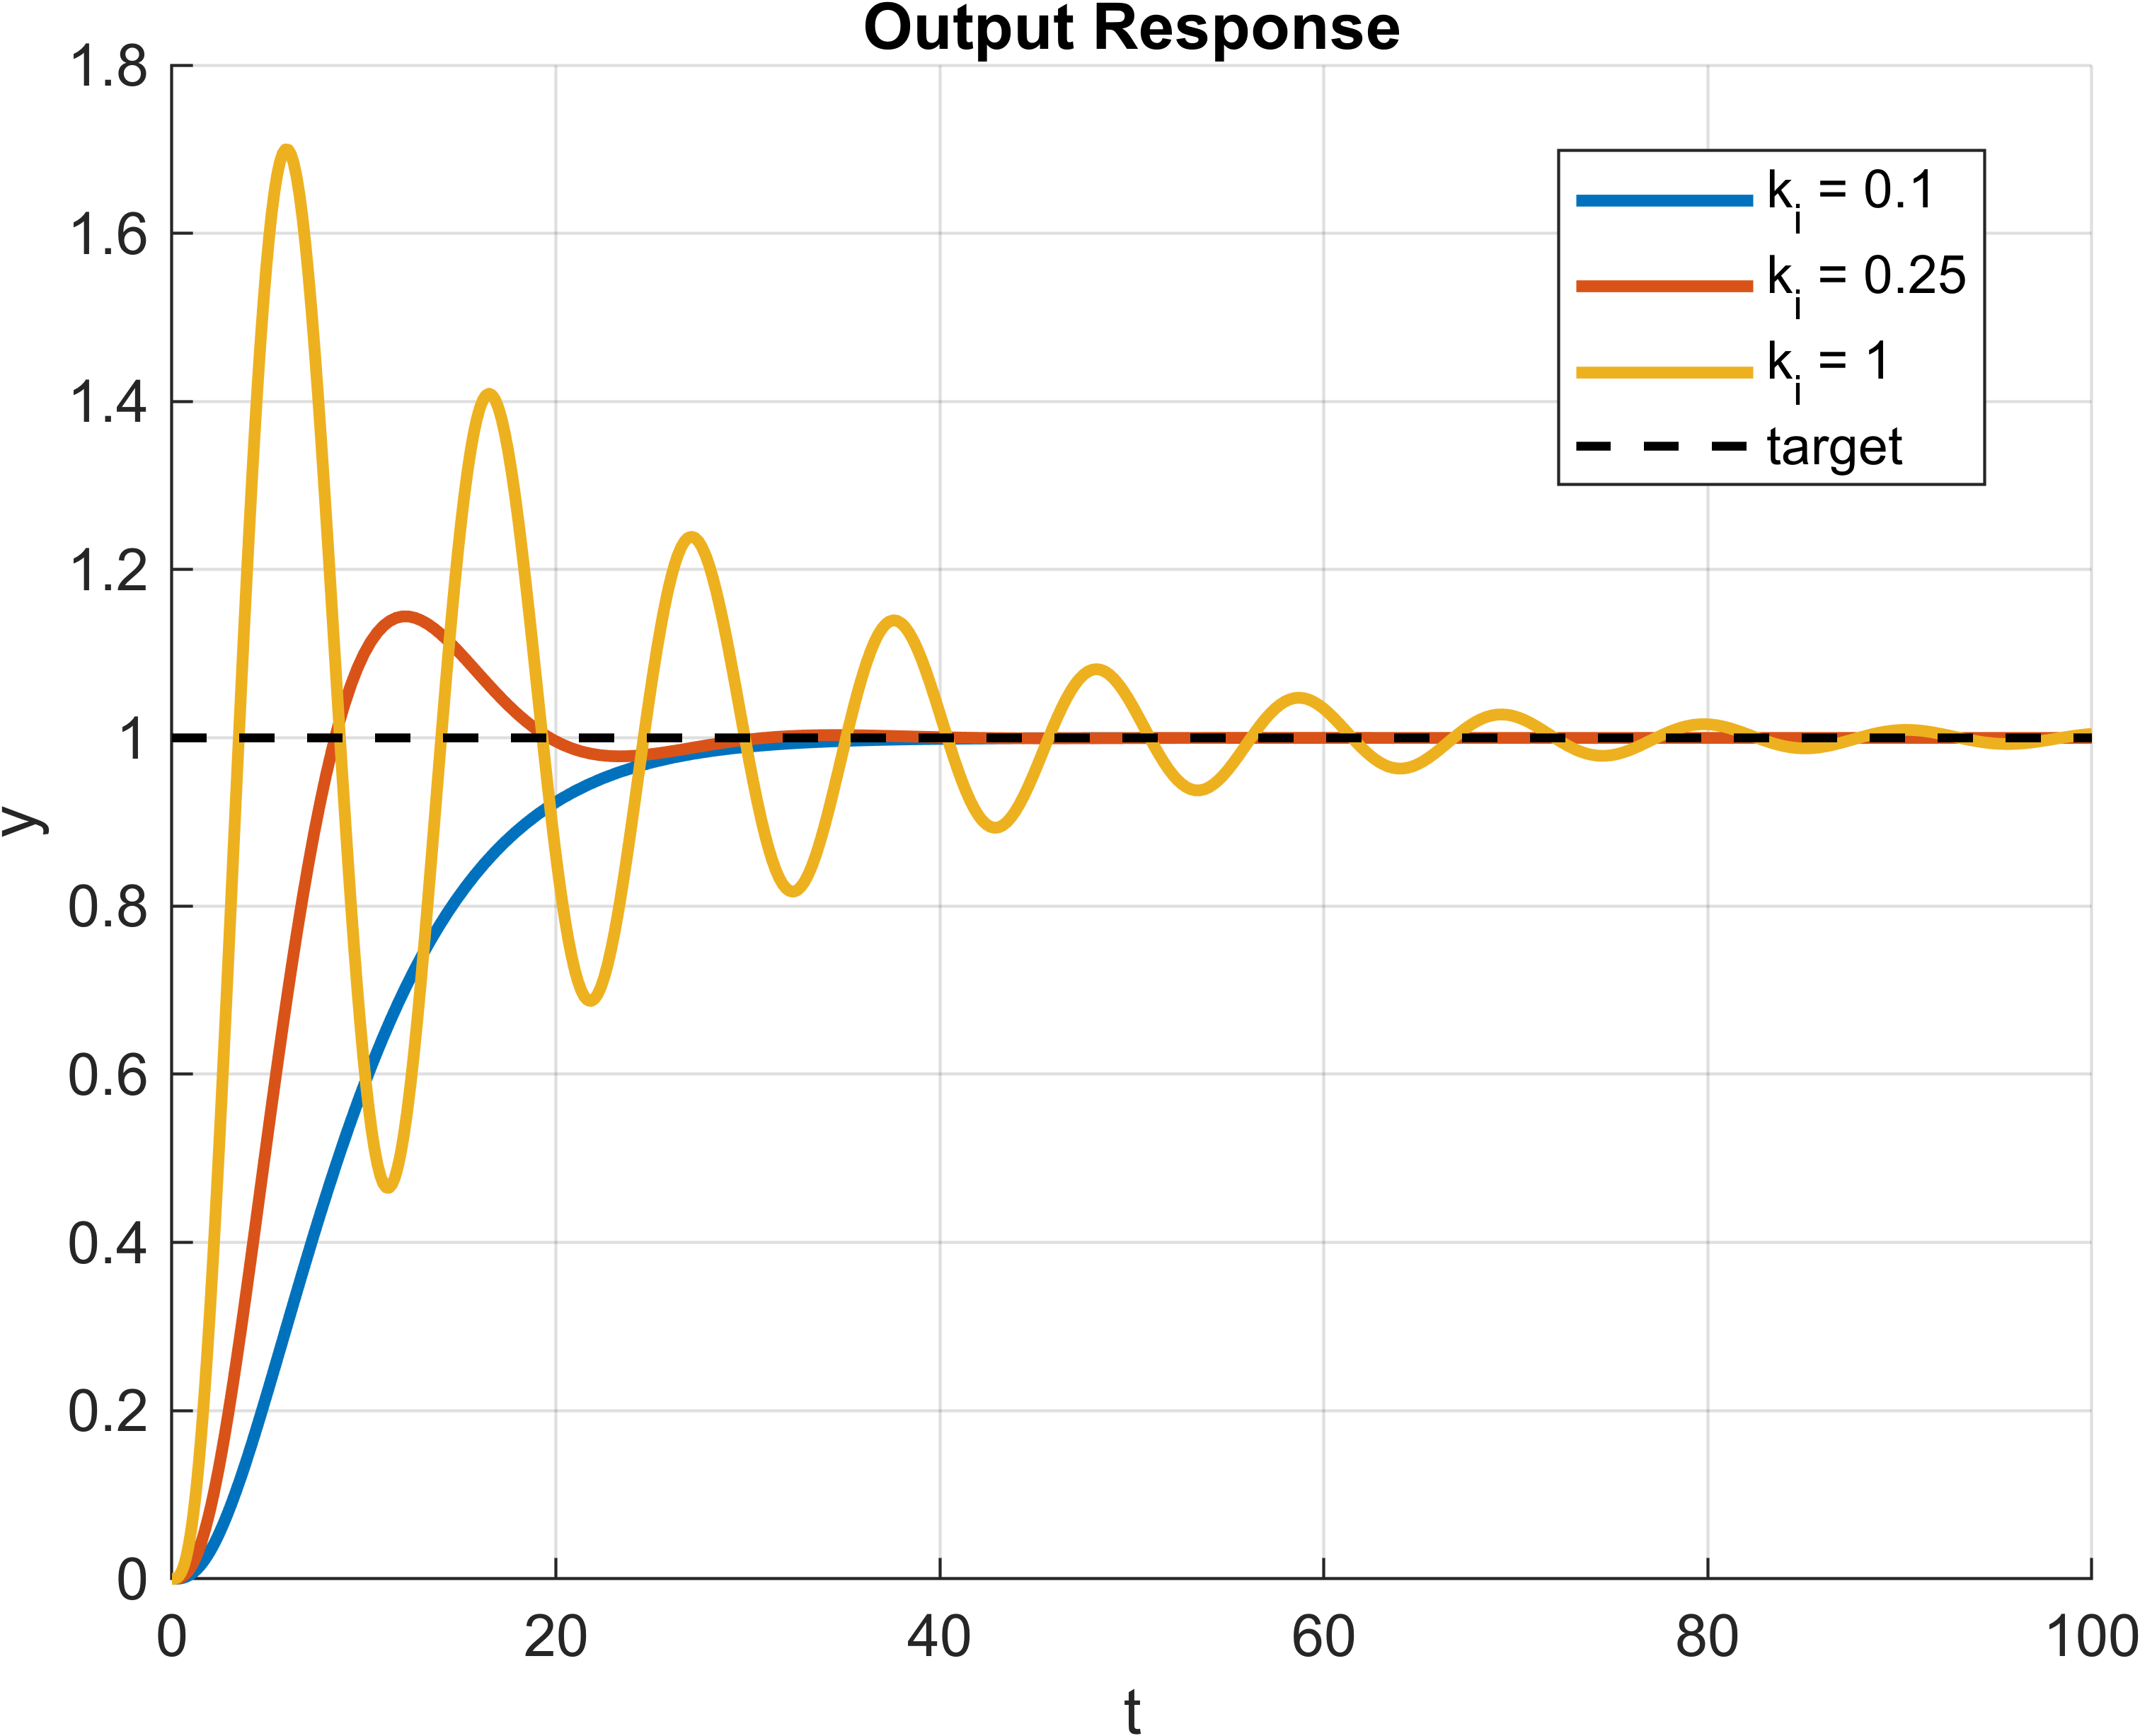
\includegraphics[width=0.75\textwidth, trim={0cm 0cm 0cm 0cm}]{../images/4_1.png}
    \caption{Переходная характеристика пружинного маятника}
\end{figure}

\begin{figure}[H]
    \centering
    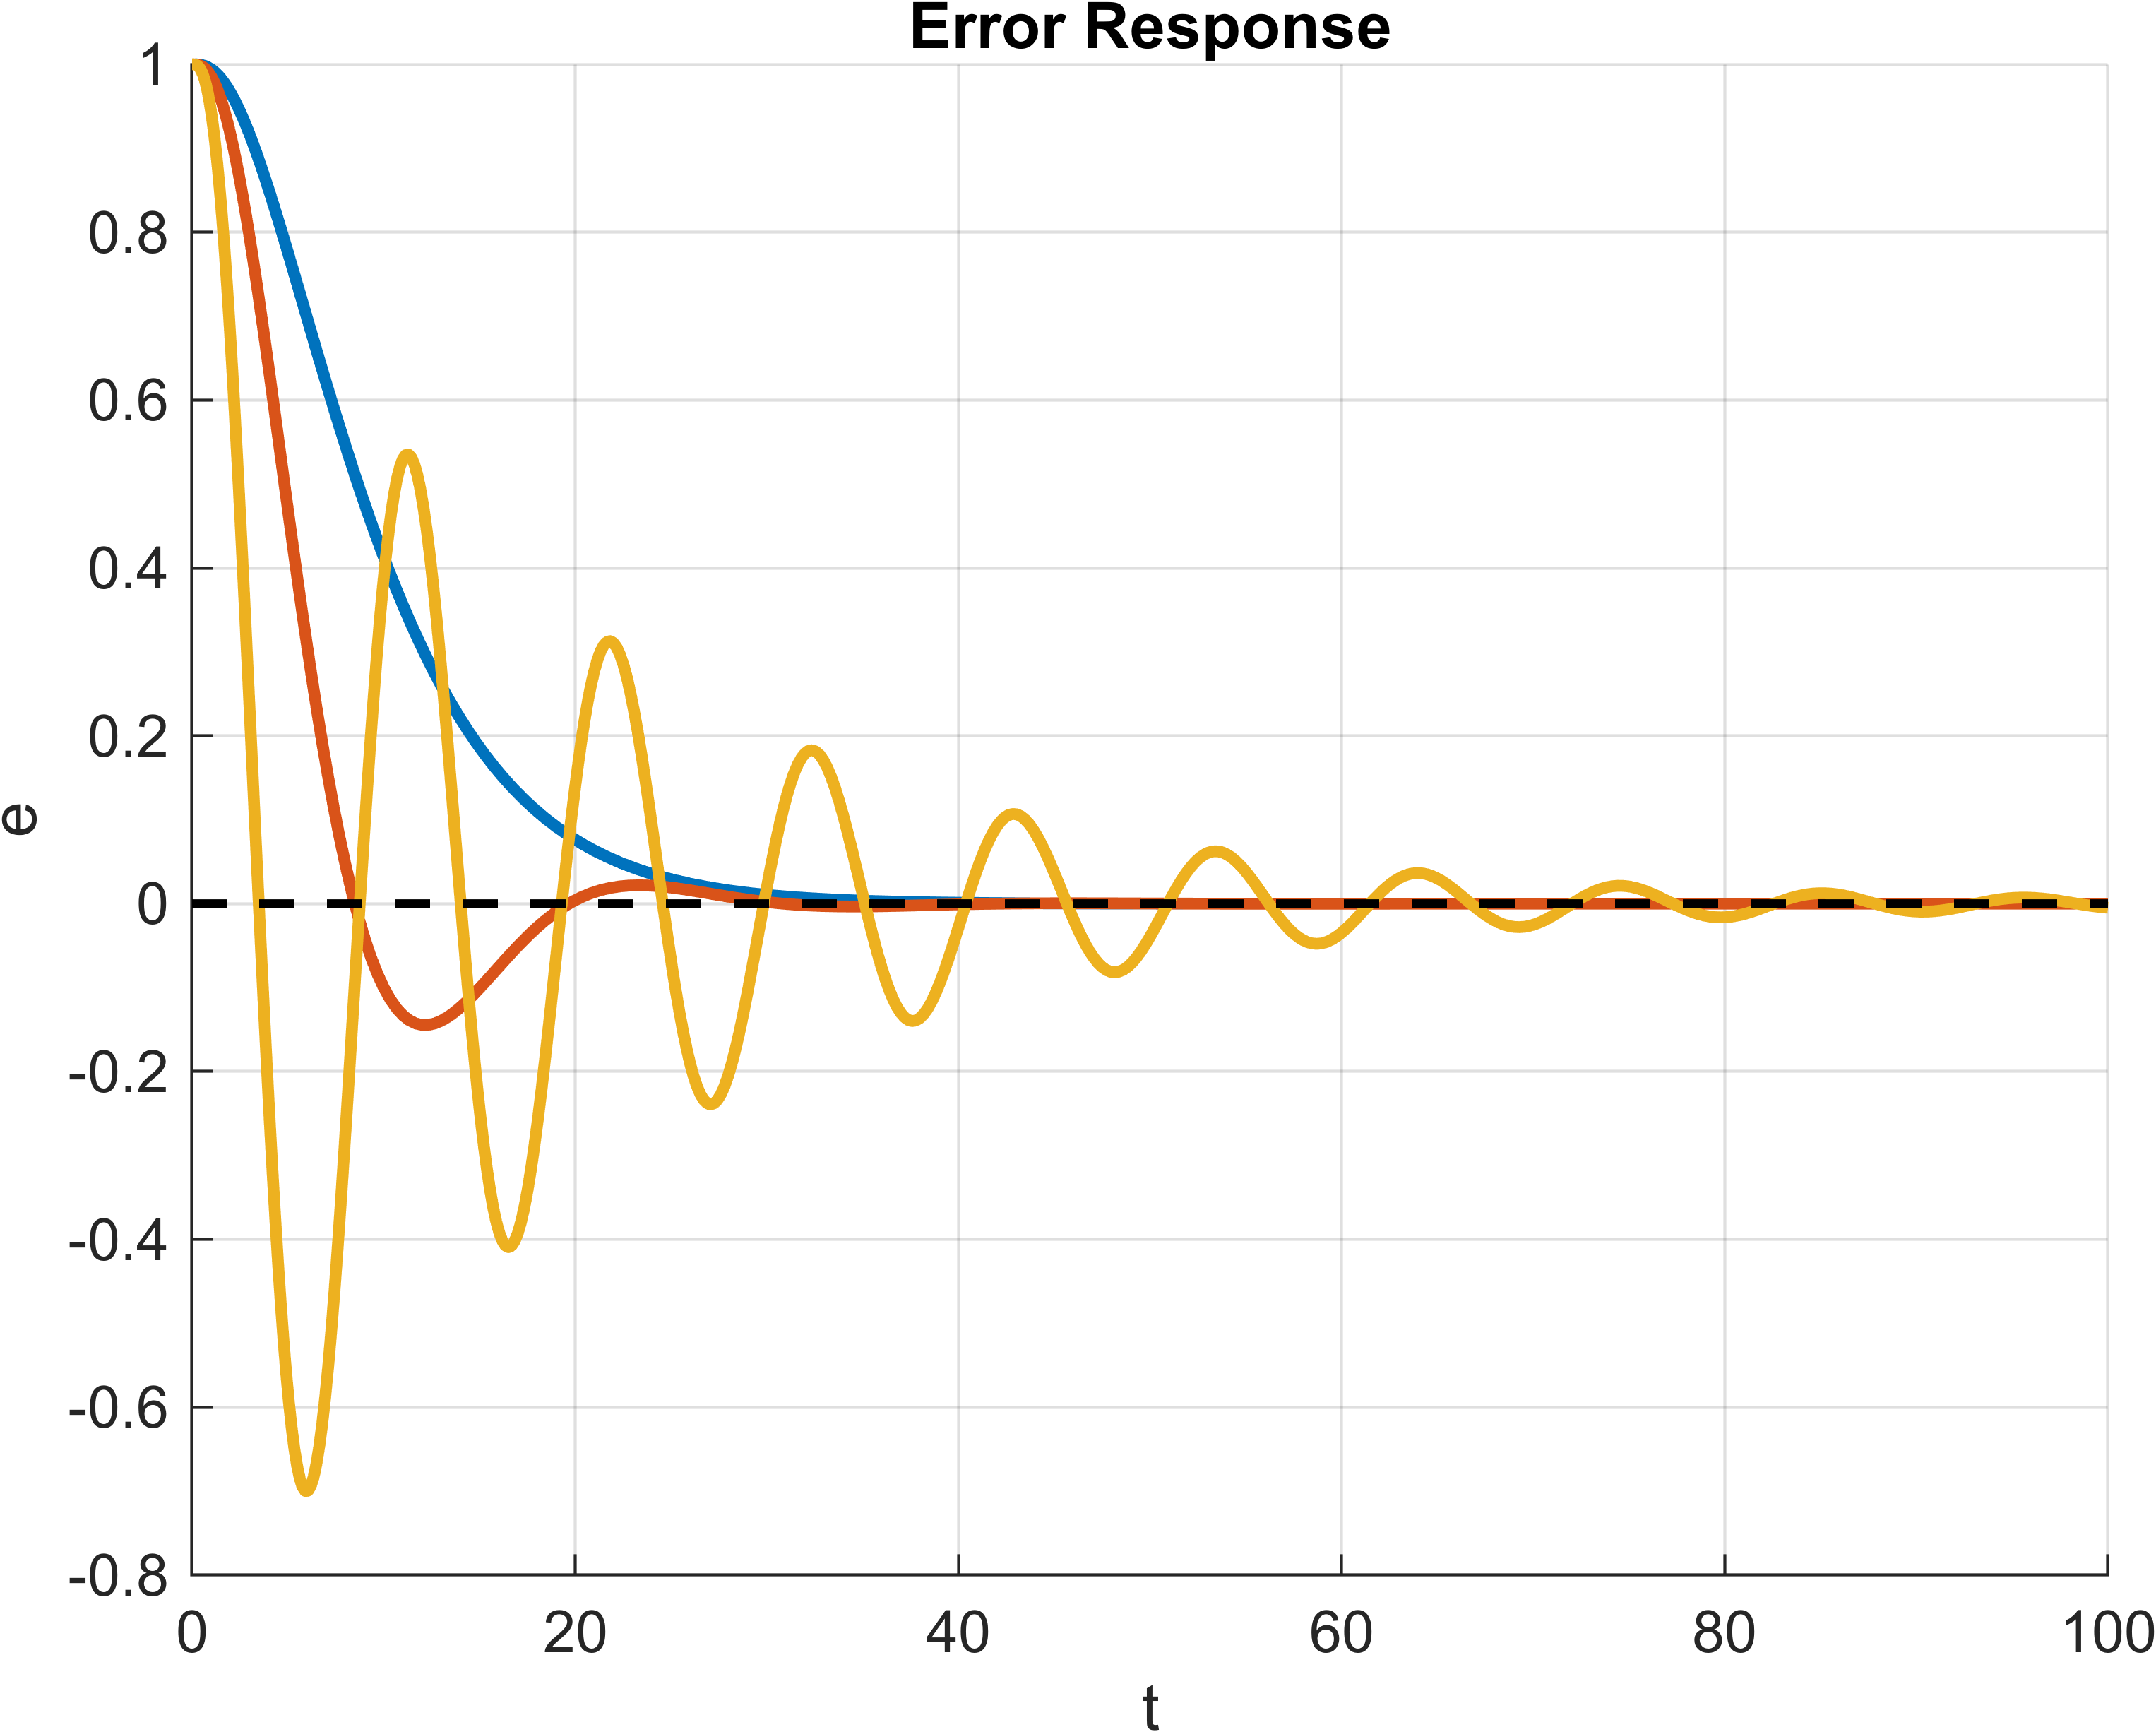
\includegraphics[width=0.75\textwidth, trim={0cm 0cm 0cm 0cm}]{../images/4_2.png}
    \caption{Весовая характеристика пружинного маятника}
\end{figure}

\section{Частотные характеристики}

Амплитудно-частотная характеристика для консервативного звена имеет вид:
\[
    A(\omega) = \frac{K}{1 - \omega^2 T^2}
\]

Логарифмическая амплитудно-частотная характеристика:
\[
    L(\omega) = 20 \lg(K) - 40 \lg(1 - \omega^2 T^2)
\]

Фазо-частотная характеристика для консервативного звена имеет вид:
\[
\varphi(\omega) = -a\pi 
\begin{cases} 
a = 0, & \omega < T^{-1} \\ 
a = 1, & \omega > T^{-1} 
\end{cases}
\]

\begin{figure}[H]
    \centering
    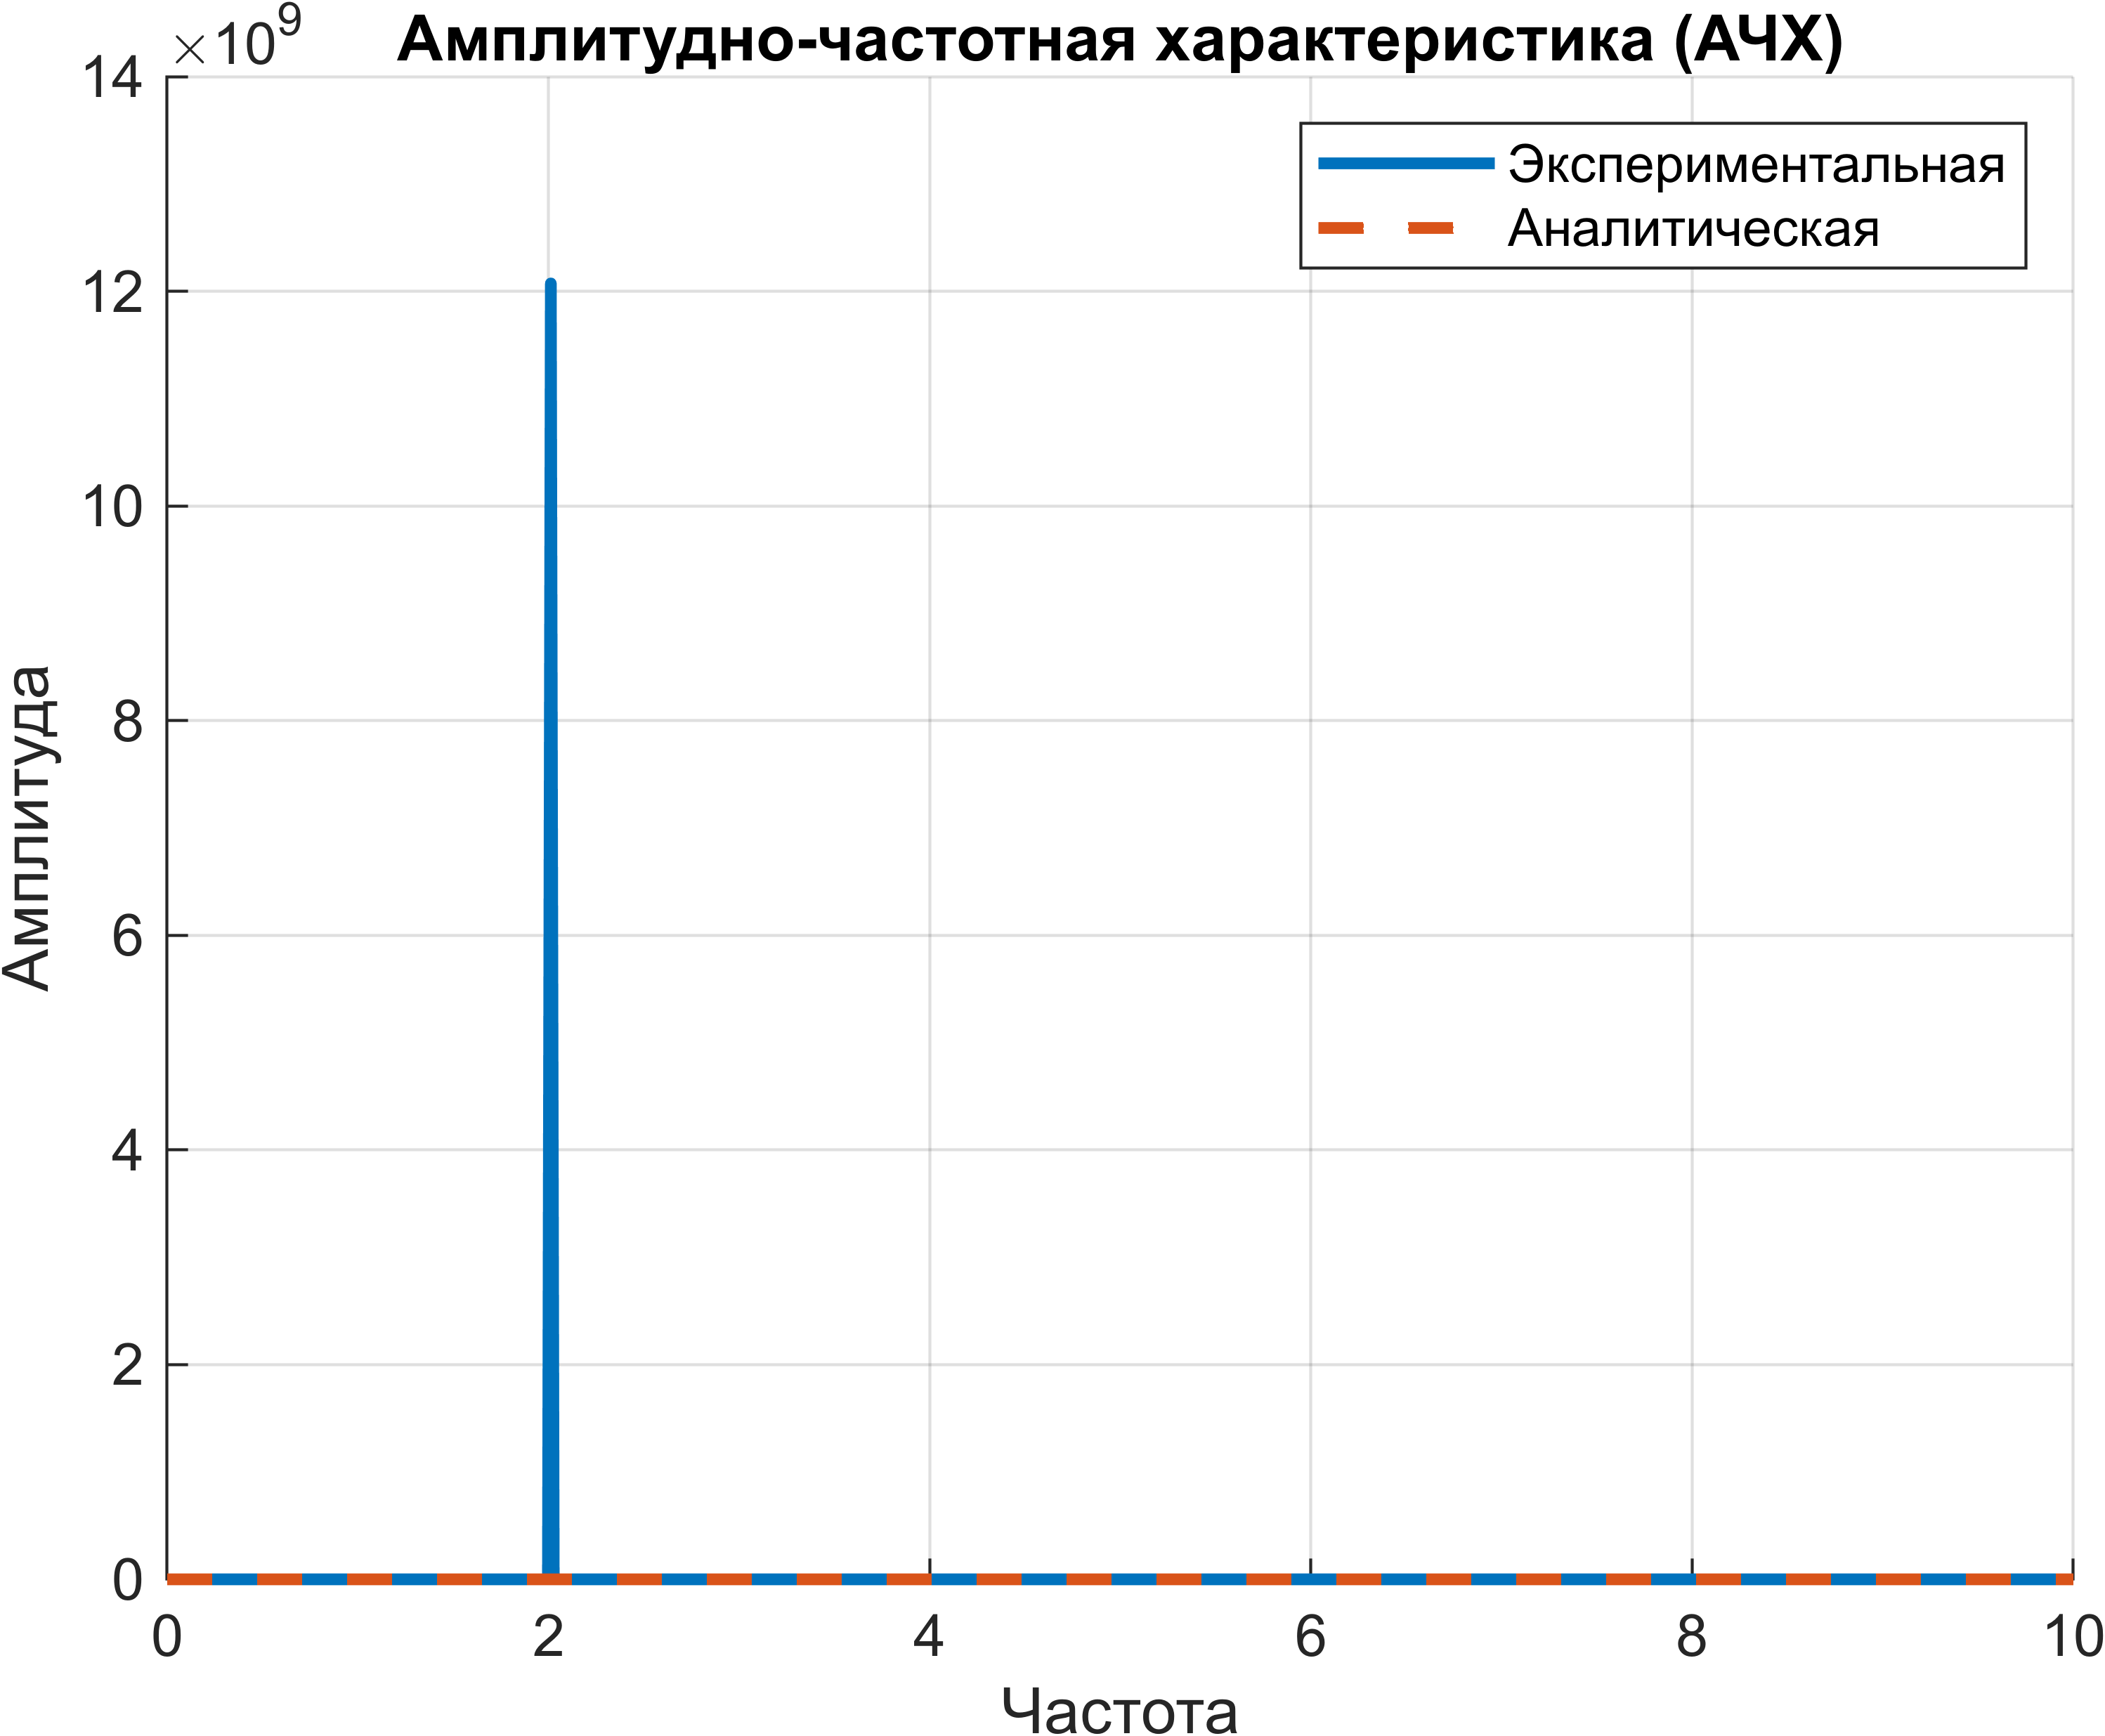
\includegraphics[width=0.75\textwidth, trim={0cm 0cm 0cm 0cm}]{../images/4_3.png}
    \caption{Амплитудно-частотная характеристика пружинного маятника}
\end{figure}

\begin{figure}[H]
    \centering
    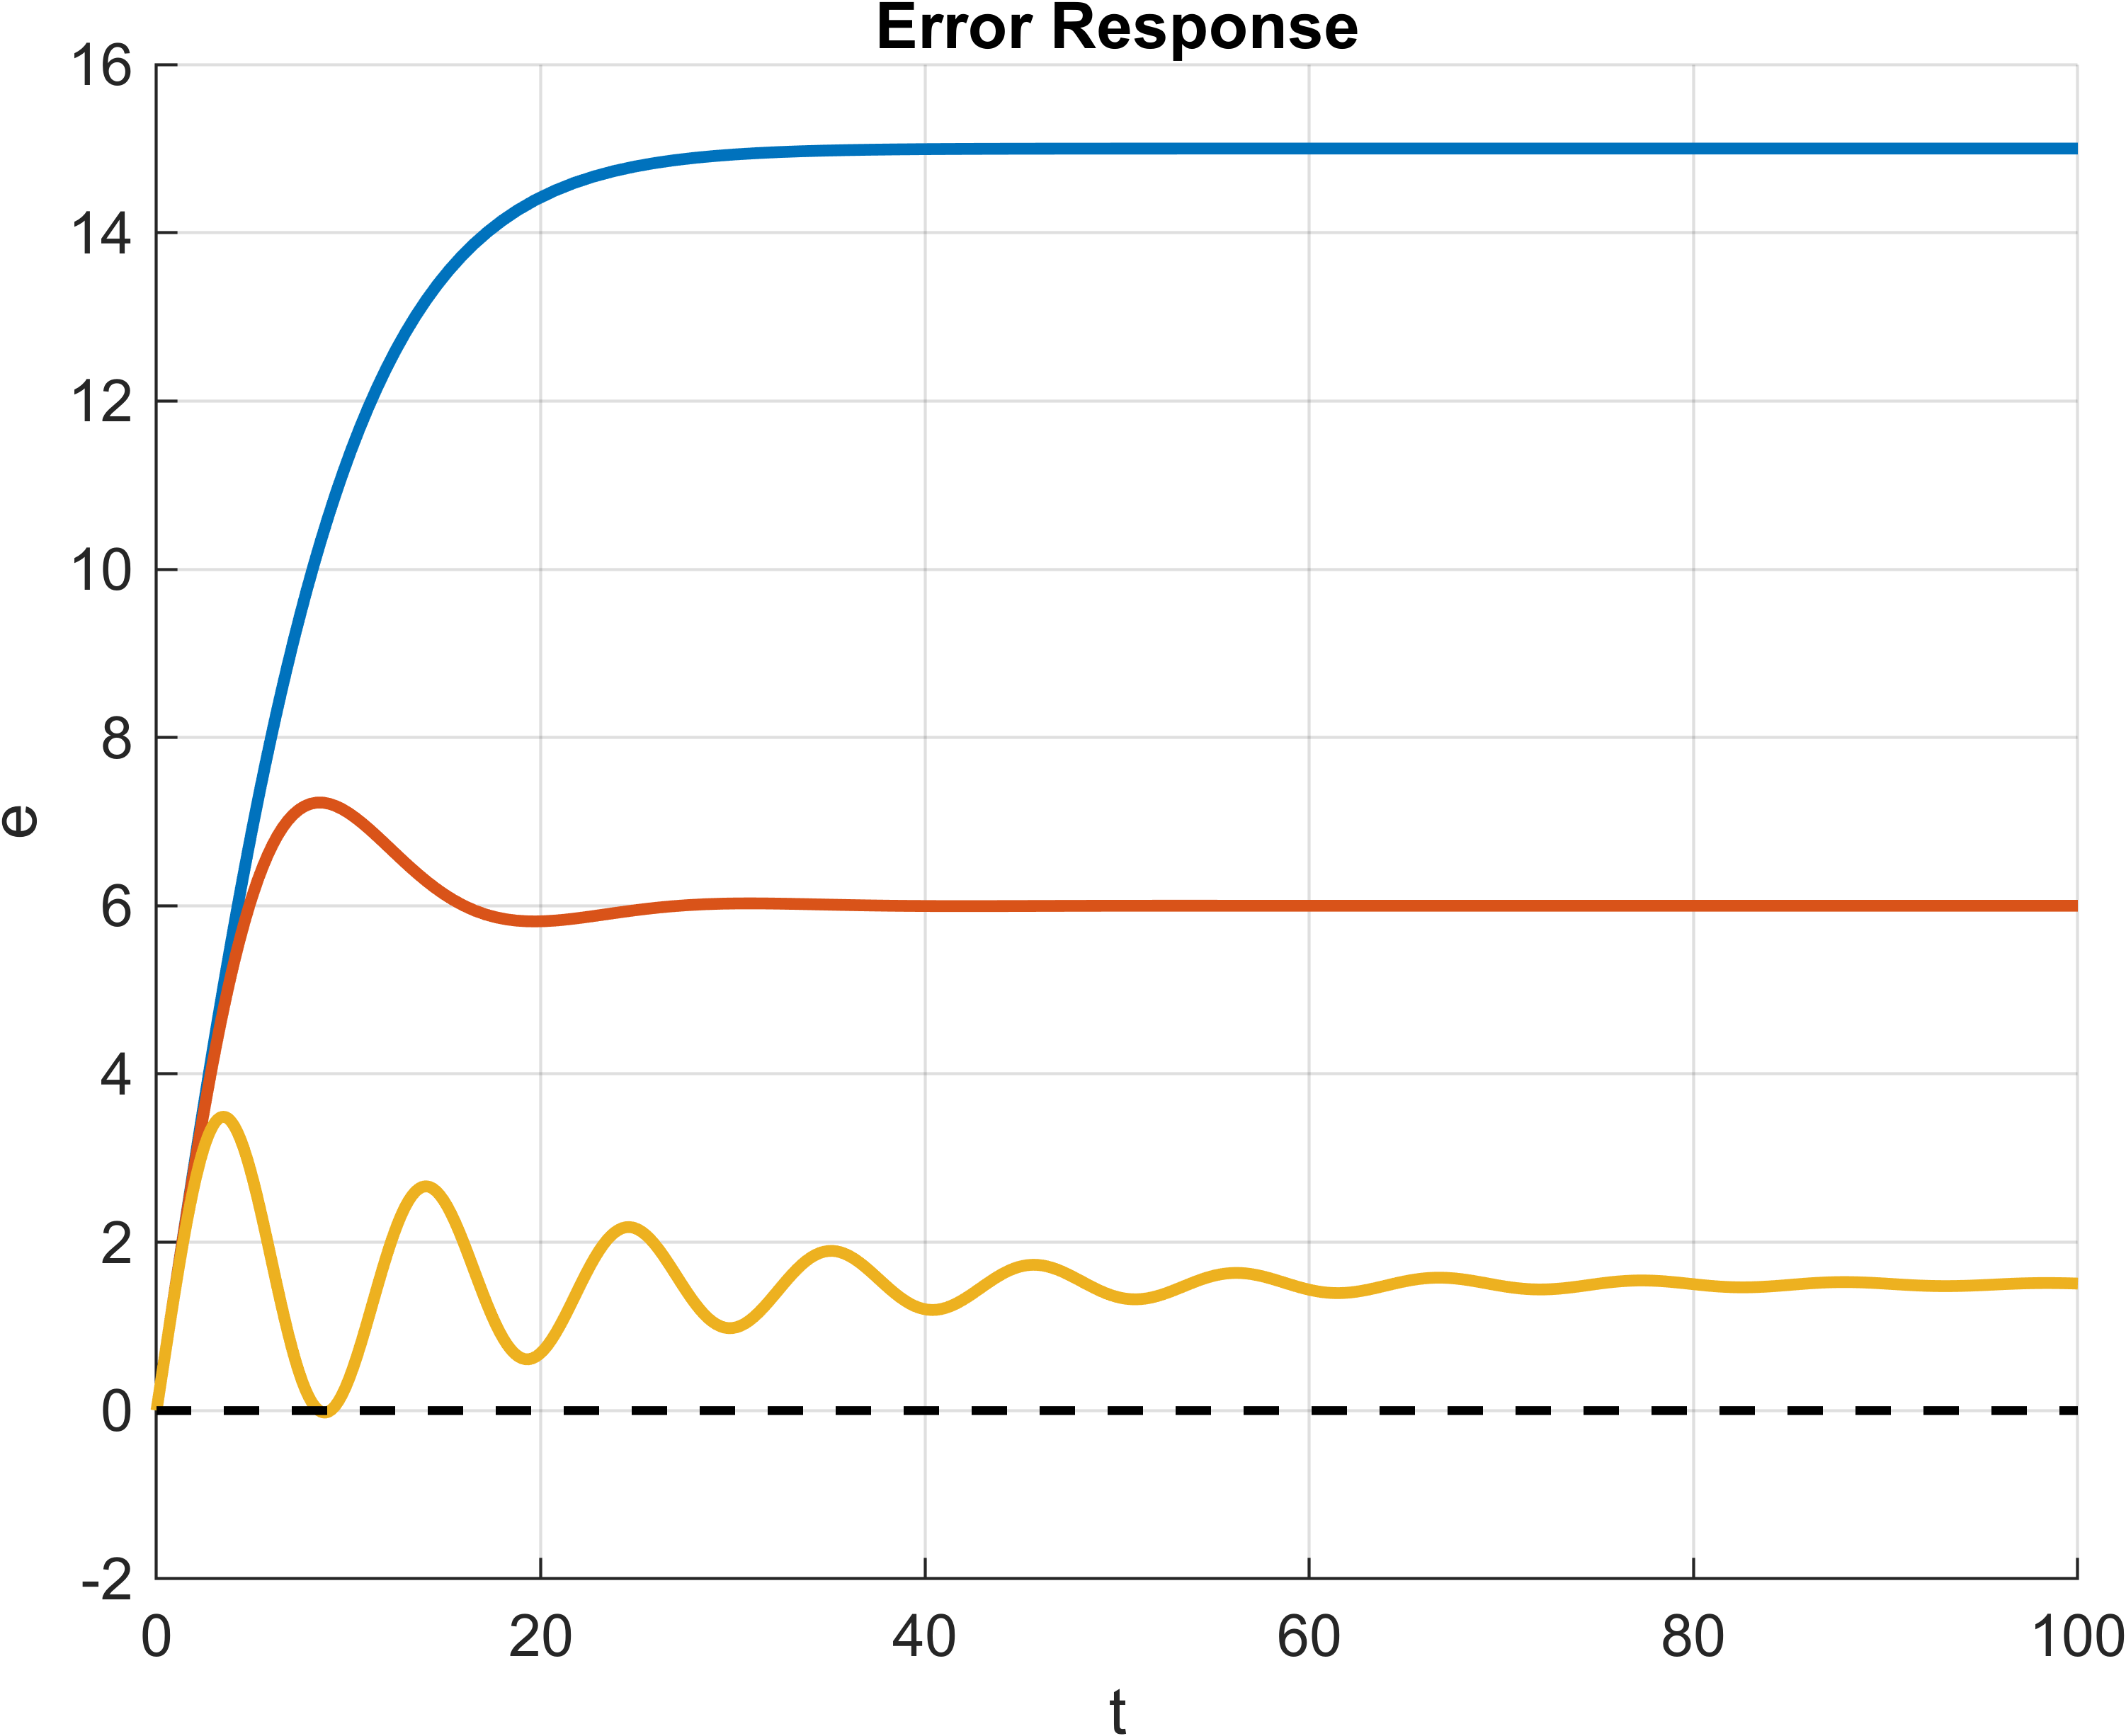
\includegraphics[width=0.75\textwidth, trim={0cm 0cm 0cm 0cm}]{../images/4_4.png}
    \caption{Фазо-частотная характеристика пружинного маятника}
\end{figure}

\begin{figure}[H]
    \centering
    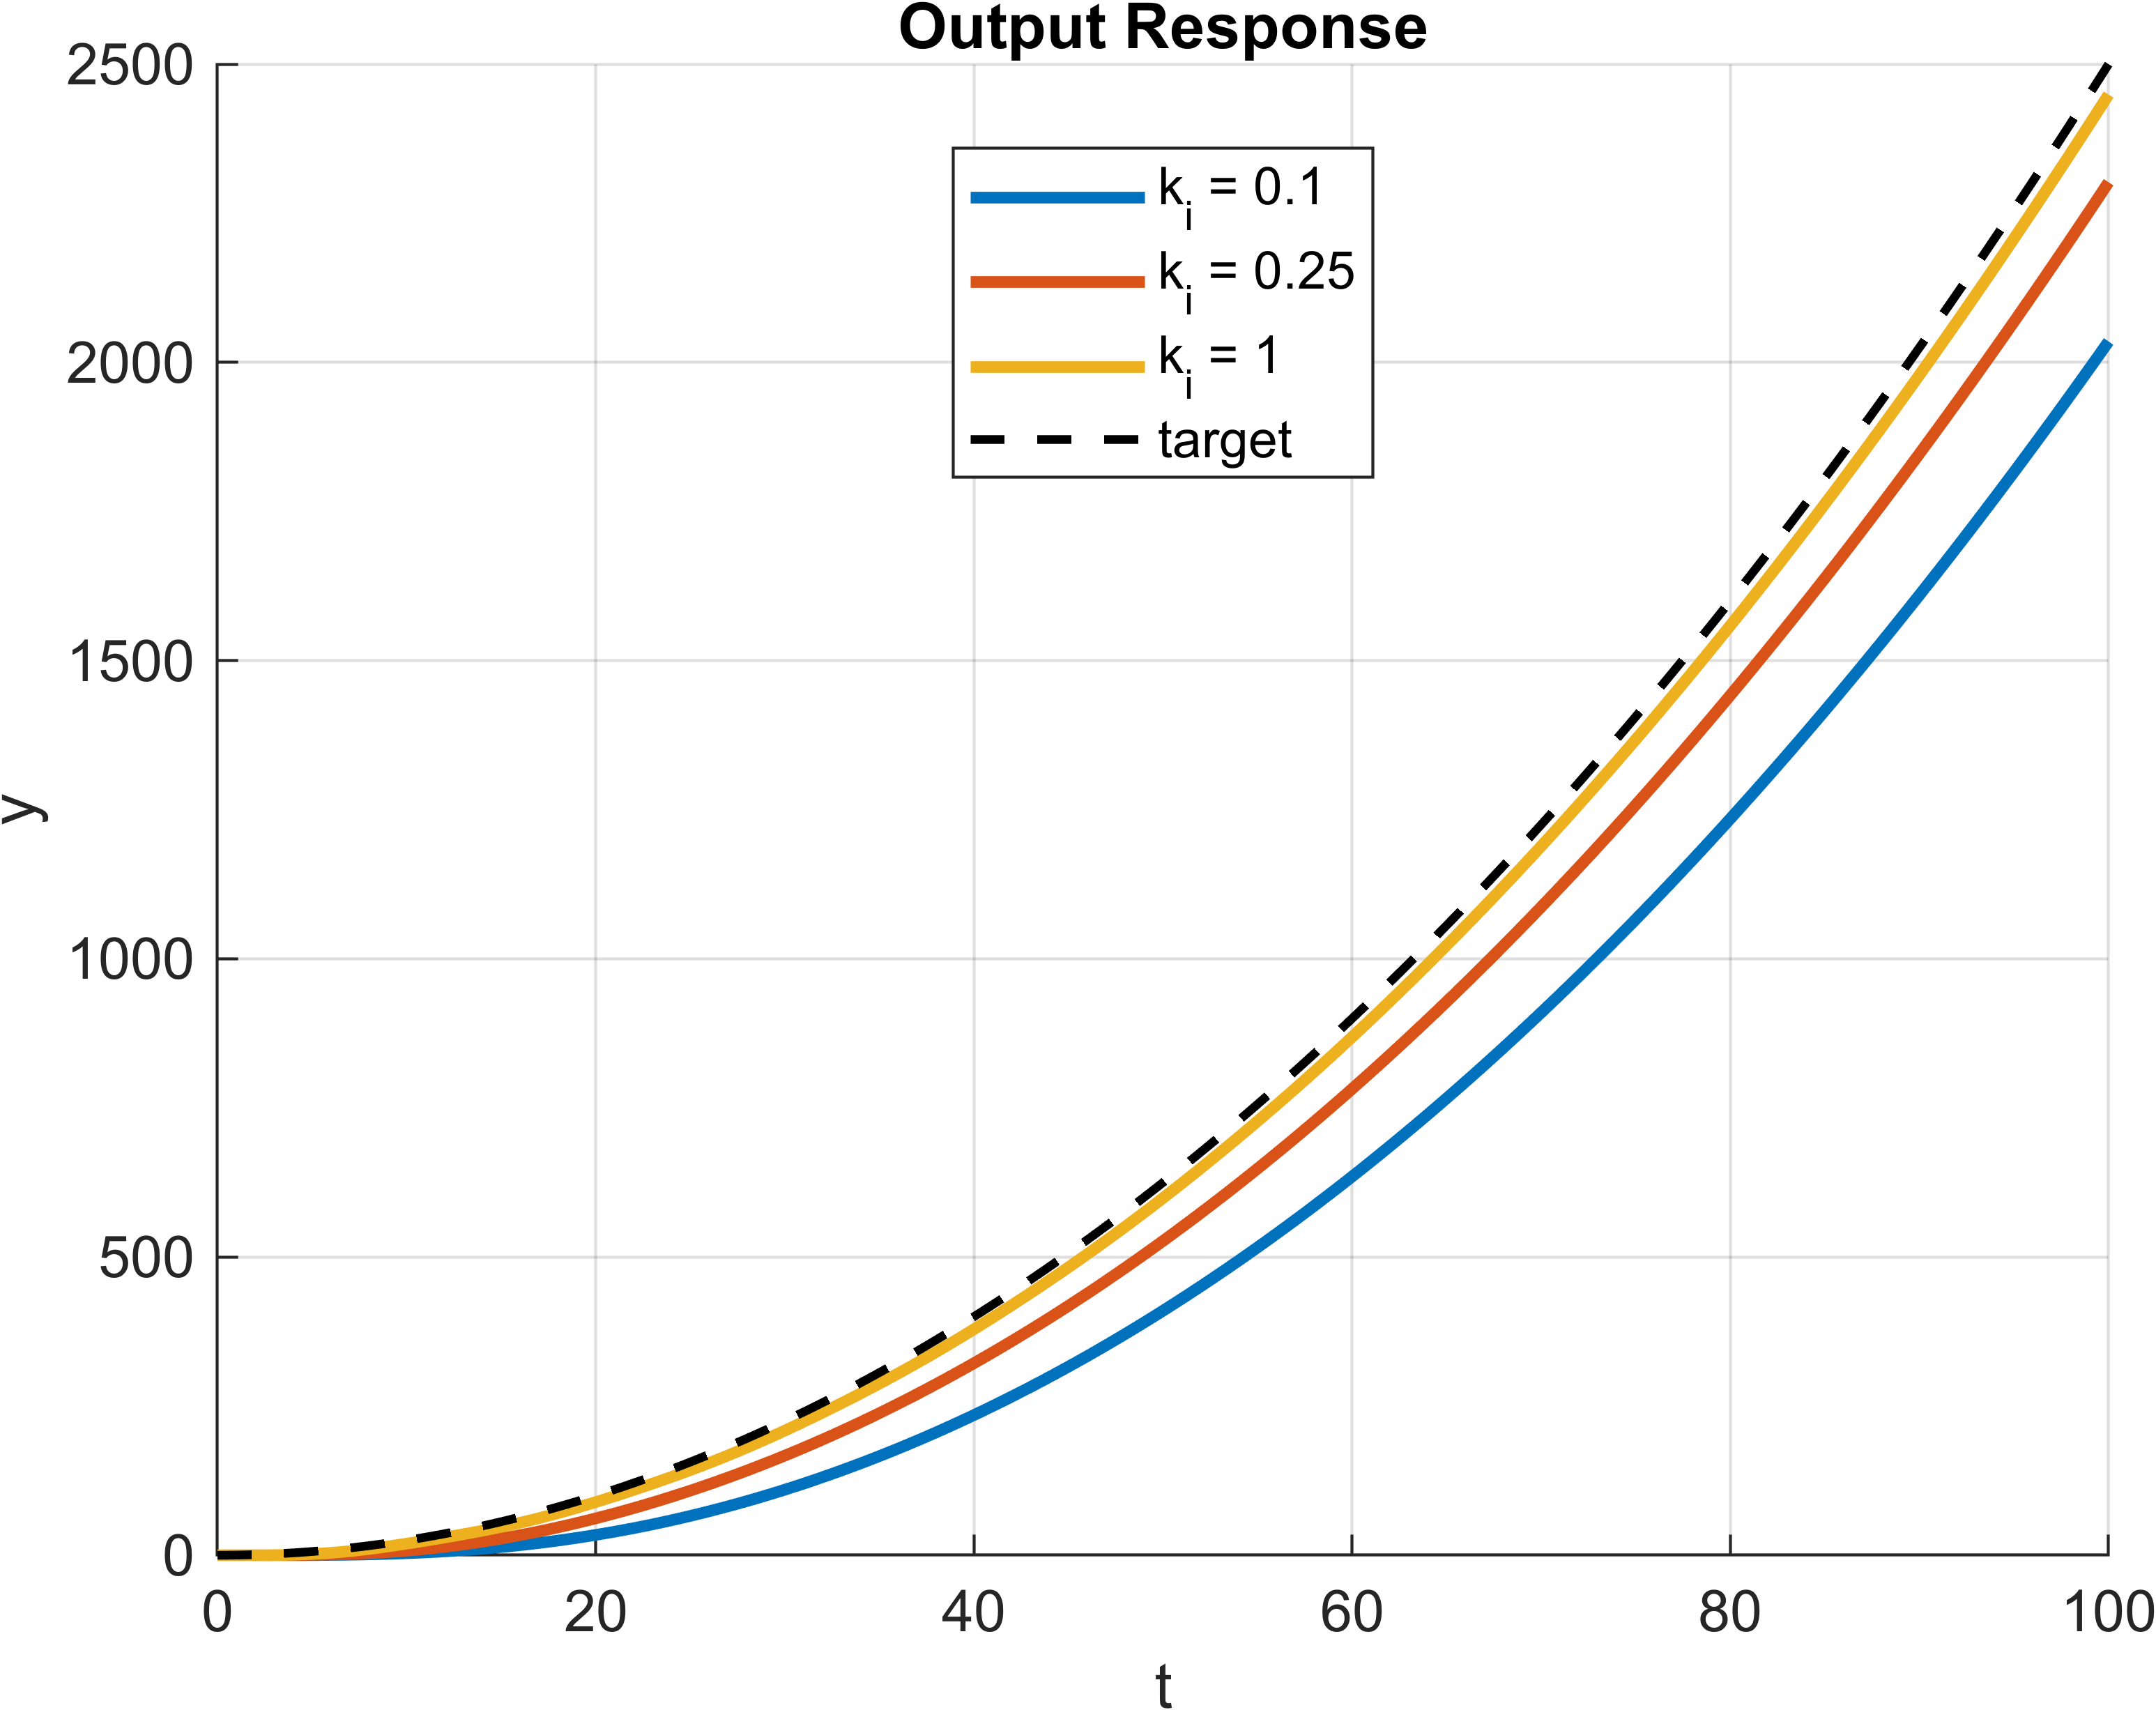
\includegraphics[width=0.75\textwidth, trim={0cm 0cm 0cm 0cm}]{../images/4_5.png}
    \caption{Логарифмическая амплитудно-фазо-частотная характеристика пружинного маятника}
\end{figure}
\endinput

% \chapter{Задача слежения для системы с астатизмом первого порядка
(ПИ-регулятор)}
Рассмотрим замкнутую систему с пропорционально-интегральным регулятором (Схема задана на рисунке
\hyperref[fig:sim4]{\ref{fig:sim4}}). Зададимся следующими парами параметрами $k_p$ и $k_i$:
\begin{itemize}
    \item $k_p = 5$, $k_p = 10$, $k_p = 25$
    \item $k_i = 0.1$, $k_i = 1$, $k_i = 5$
\end{itemize}
\section{Режим движения с постоянной скоростью $g(t) = Vt$}
Выполним моделирование:
\begin{figure}[H]
    \centering
    \begin{minipage}{0.45\textwidth}
        \centering
        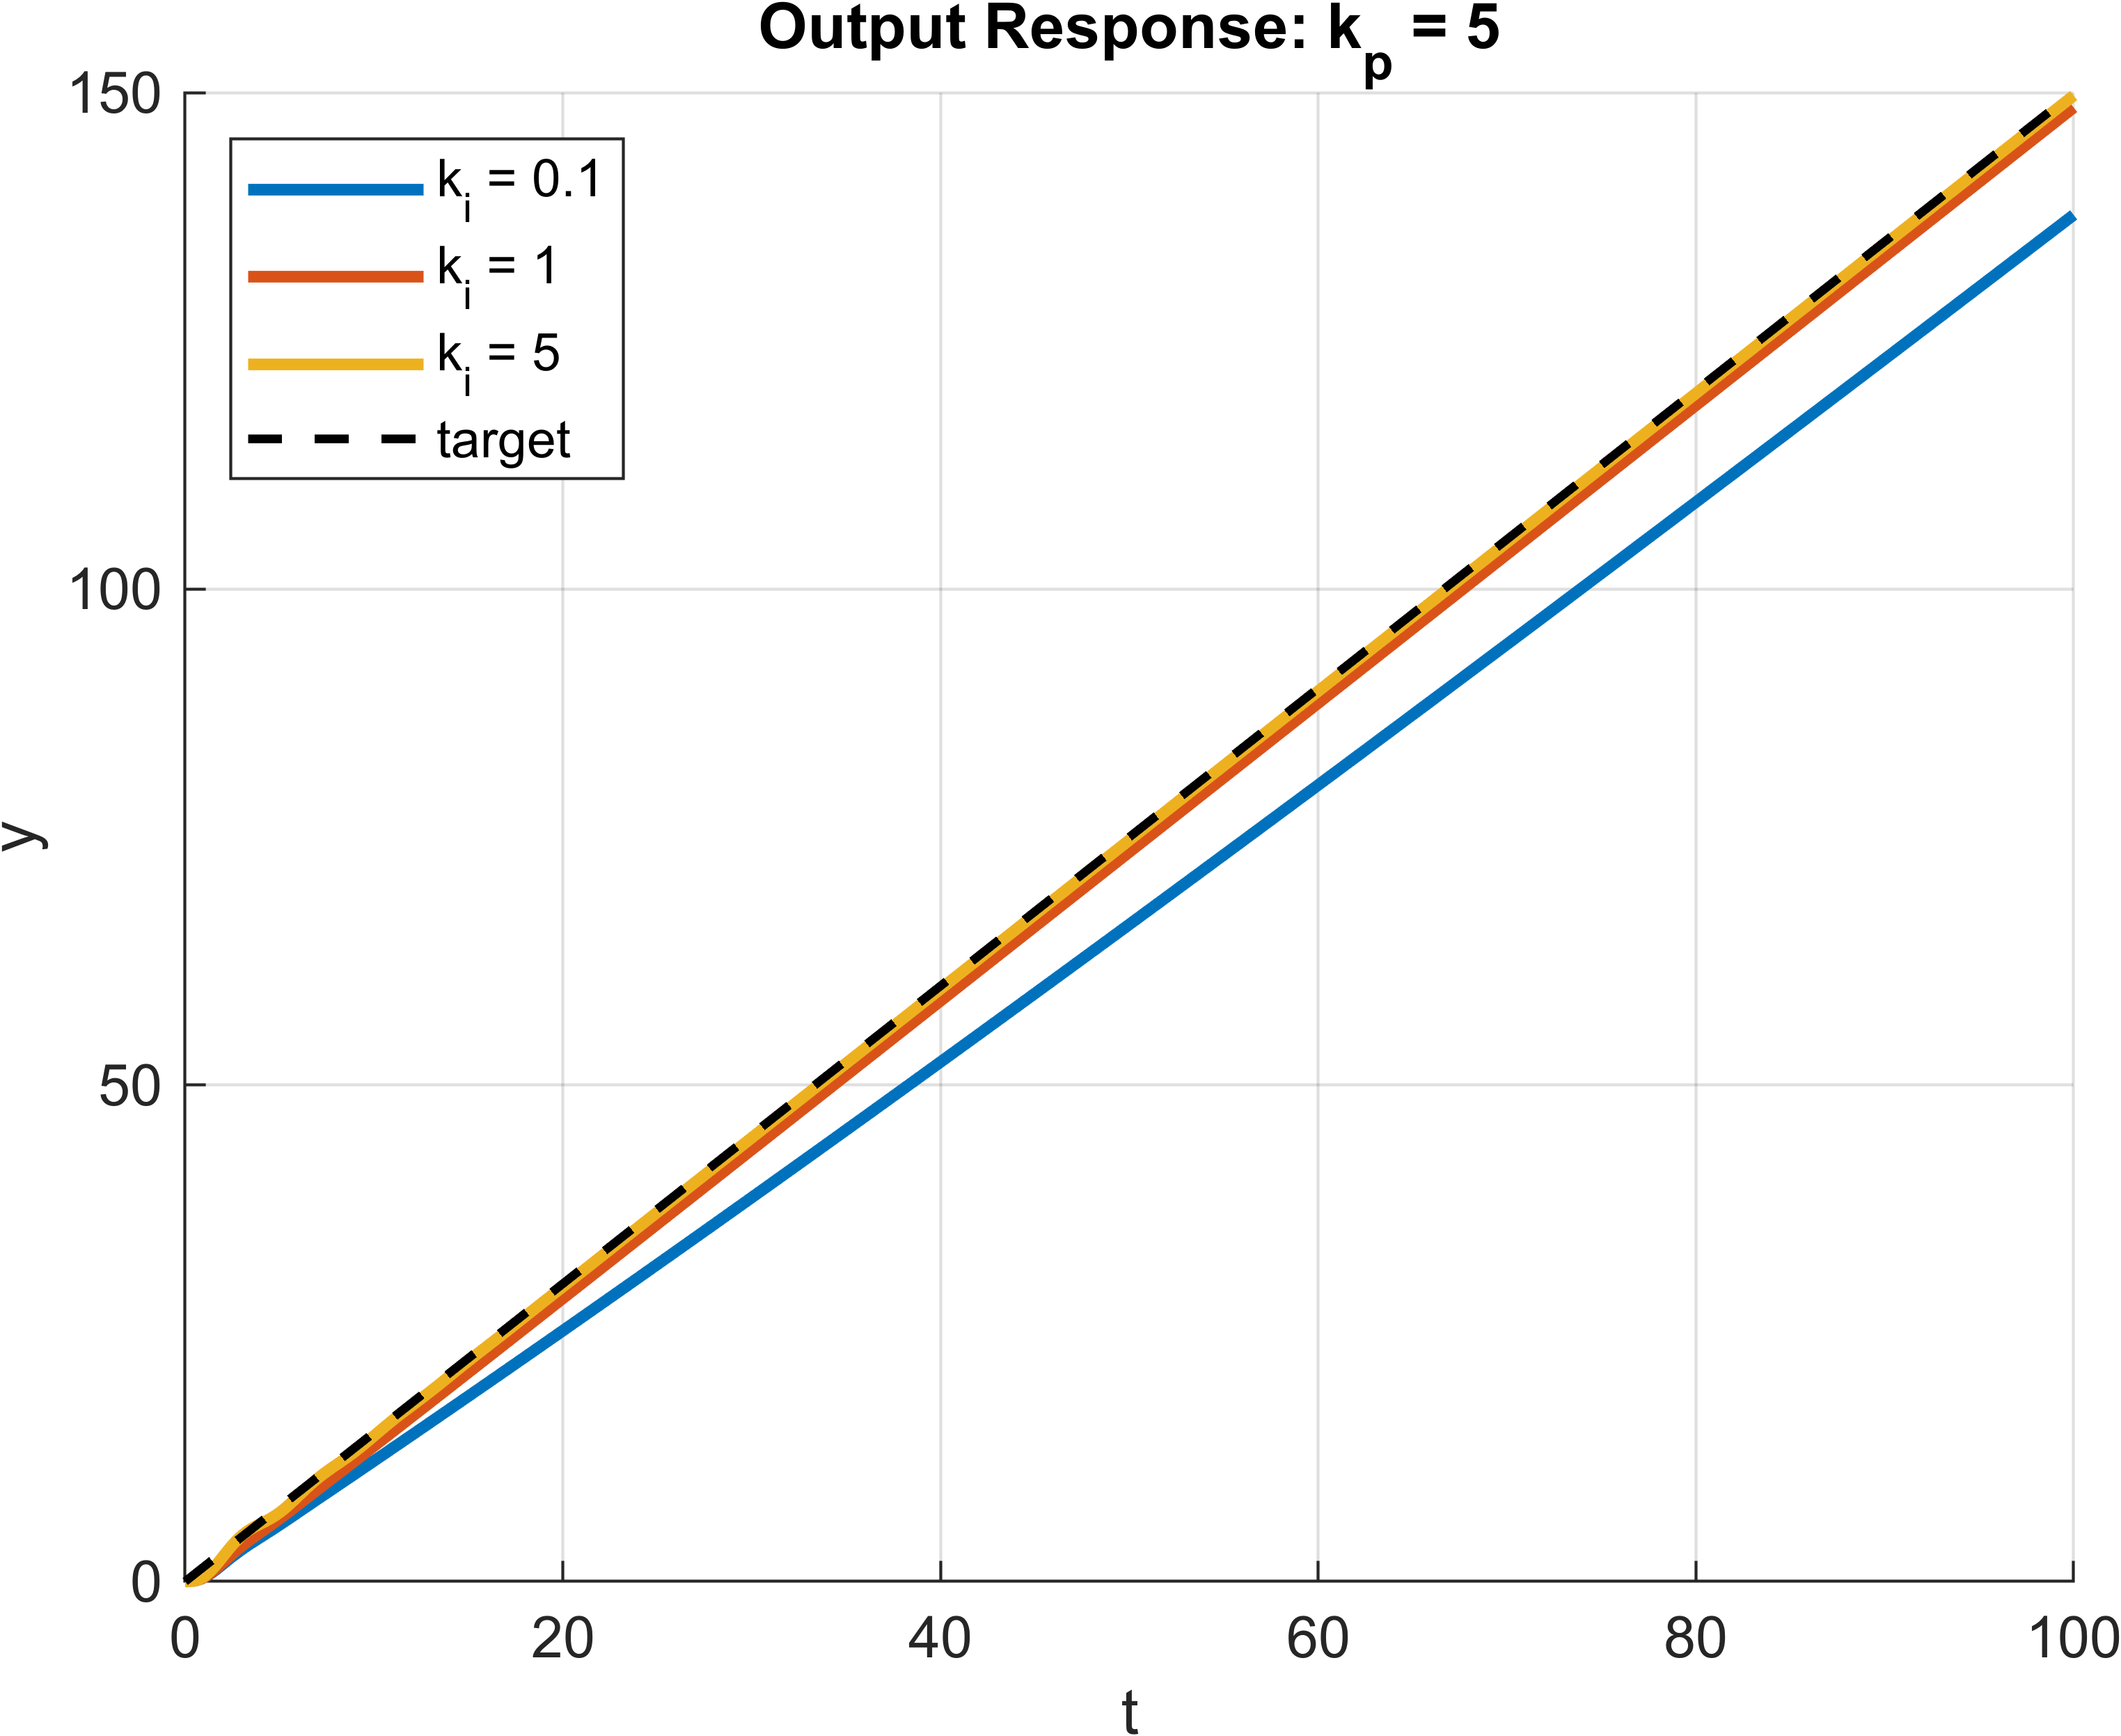
\includegraphics[width=1\textwidth, trim={1cm 0cm 1cm 0cm}]{../images/input_2_kp_5_output.png}
    \end{minipage}
    \hfill
    \begin{minipage}{0.45\textwidth}
        \centering
        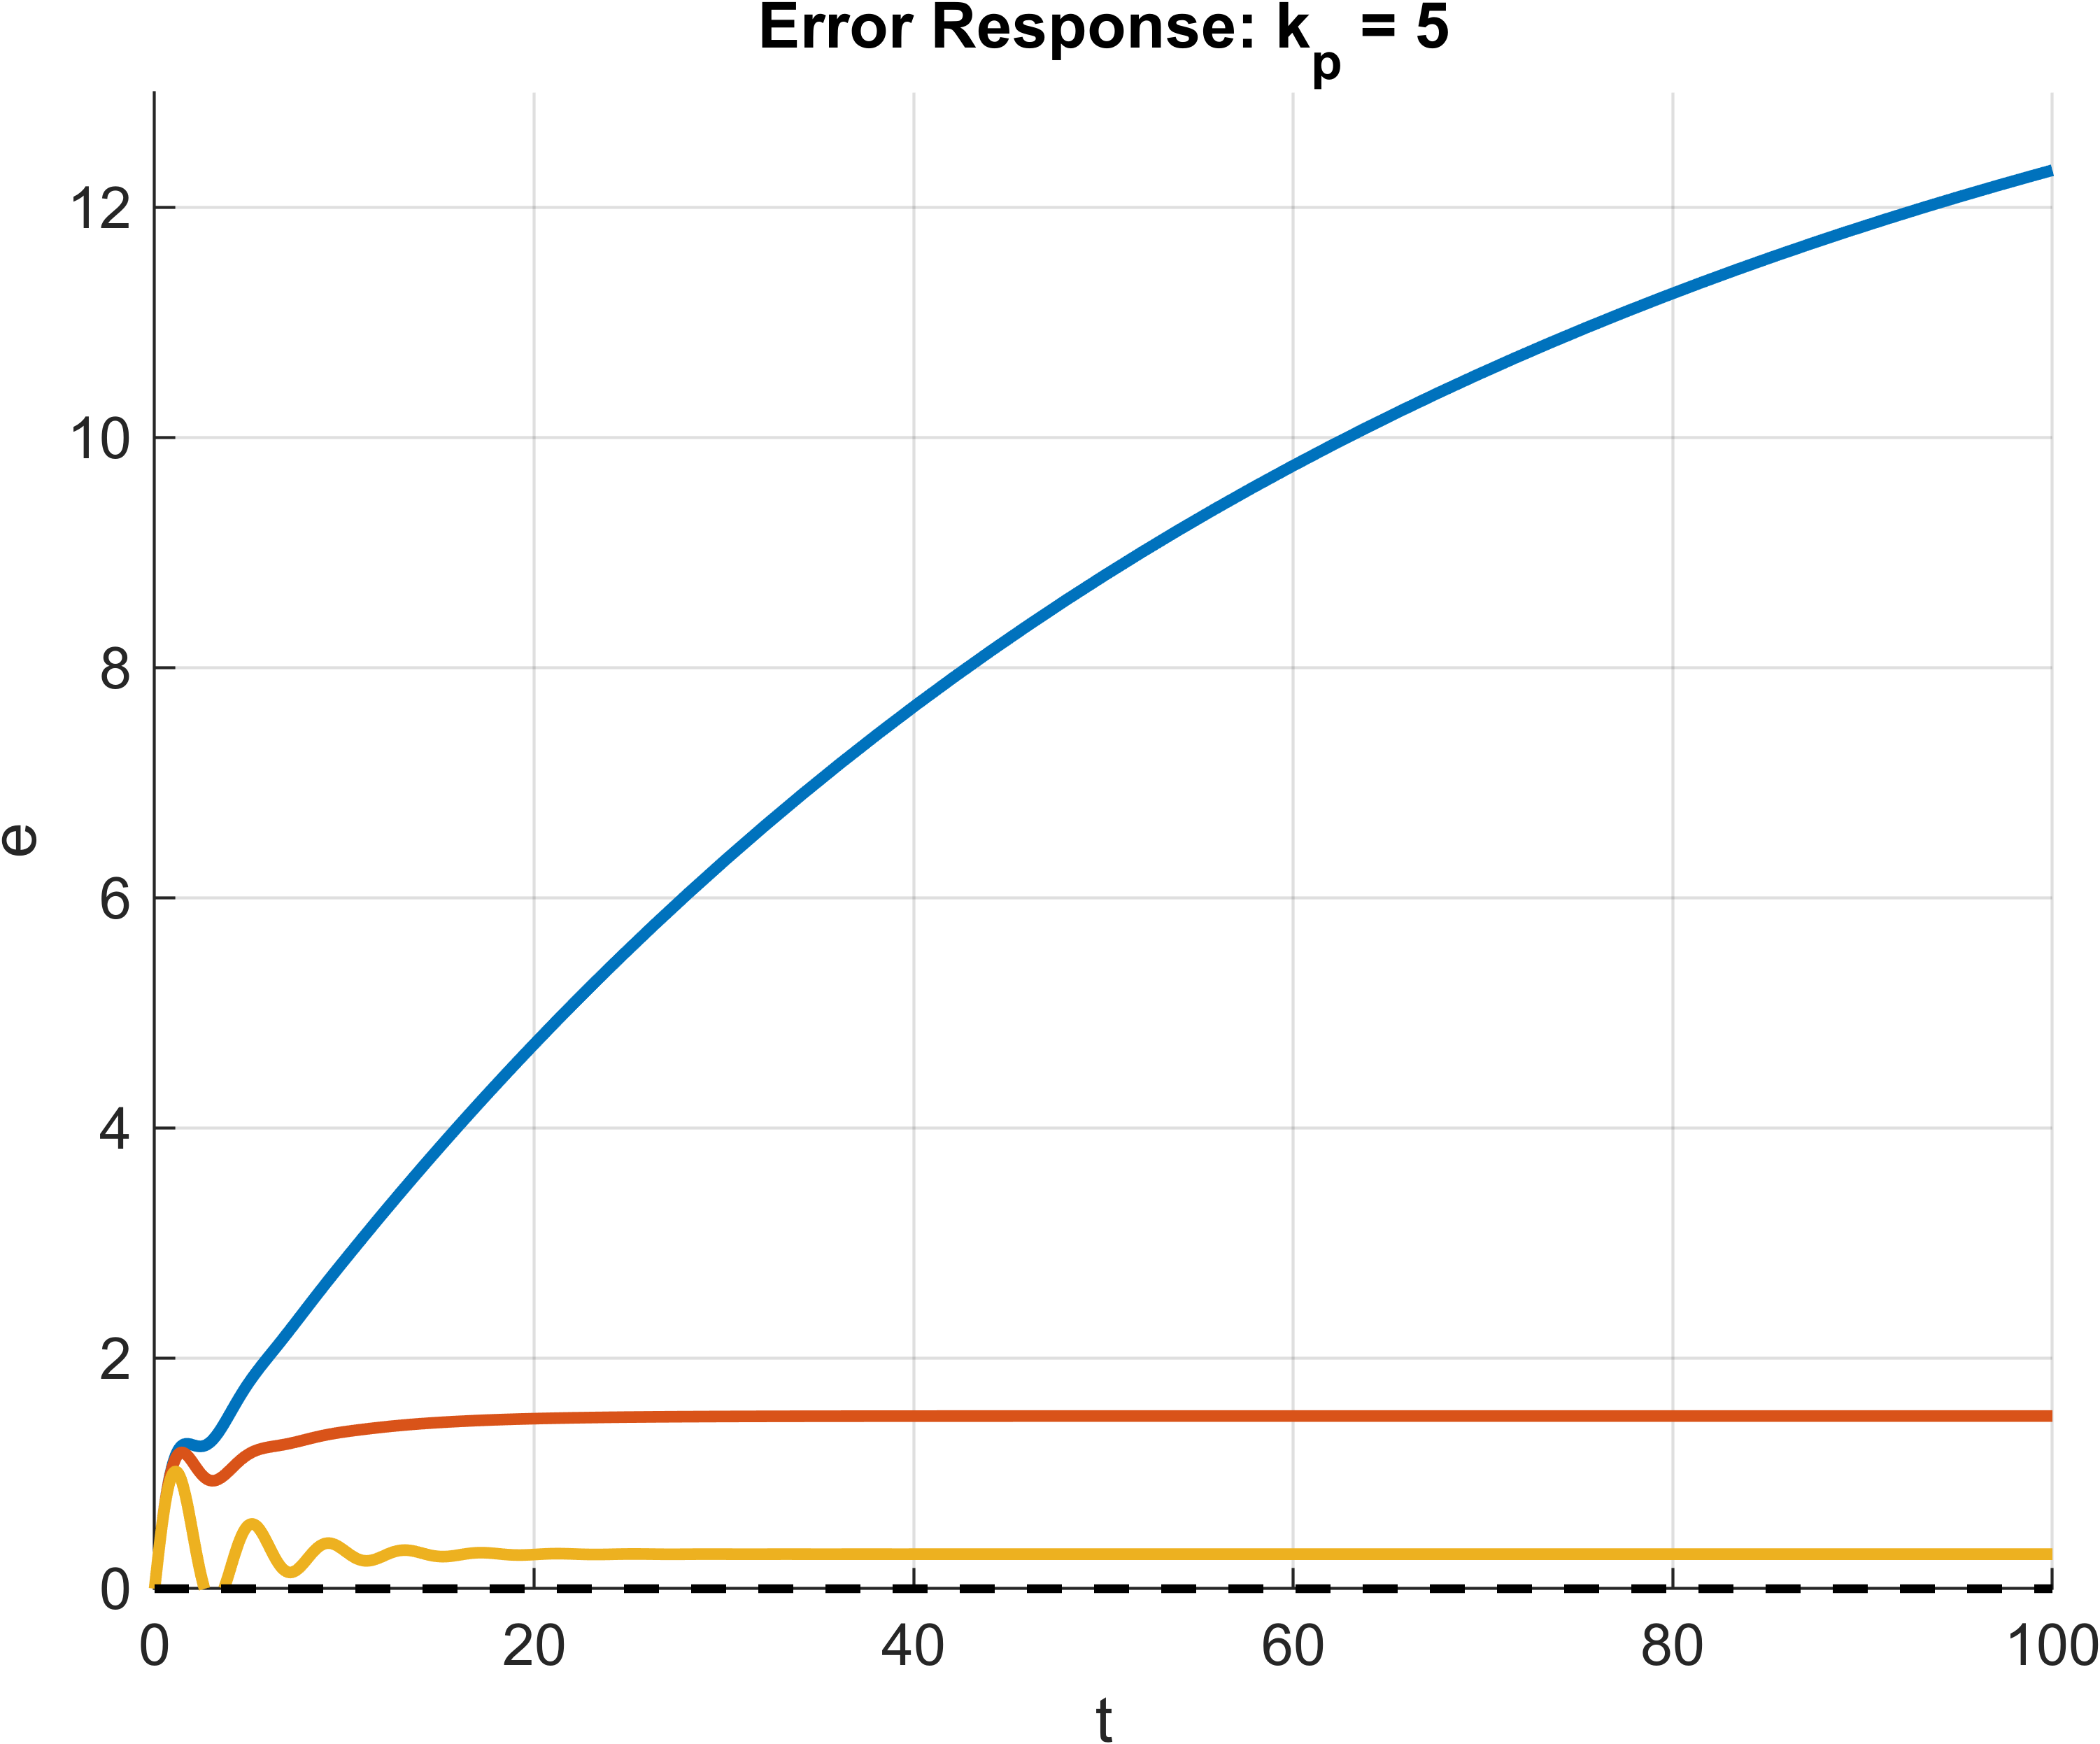
\includegraphics[width=1\textwidth, trim={1cm 0cm 1cm 0cm}]{../images/input_2_kp_5_error.png}
    \end{minipage}
    \caption{Графики $y(t)$ и $e(t)$ при $g(t) = 1.5t$ и $k_p = 5$}
\end{figure}
\begin{figure}[H]
    \centering
    \begin{minipage}{0.45\textwidth}
        \centering
        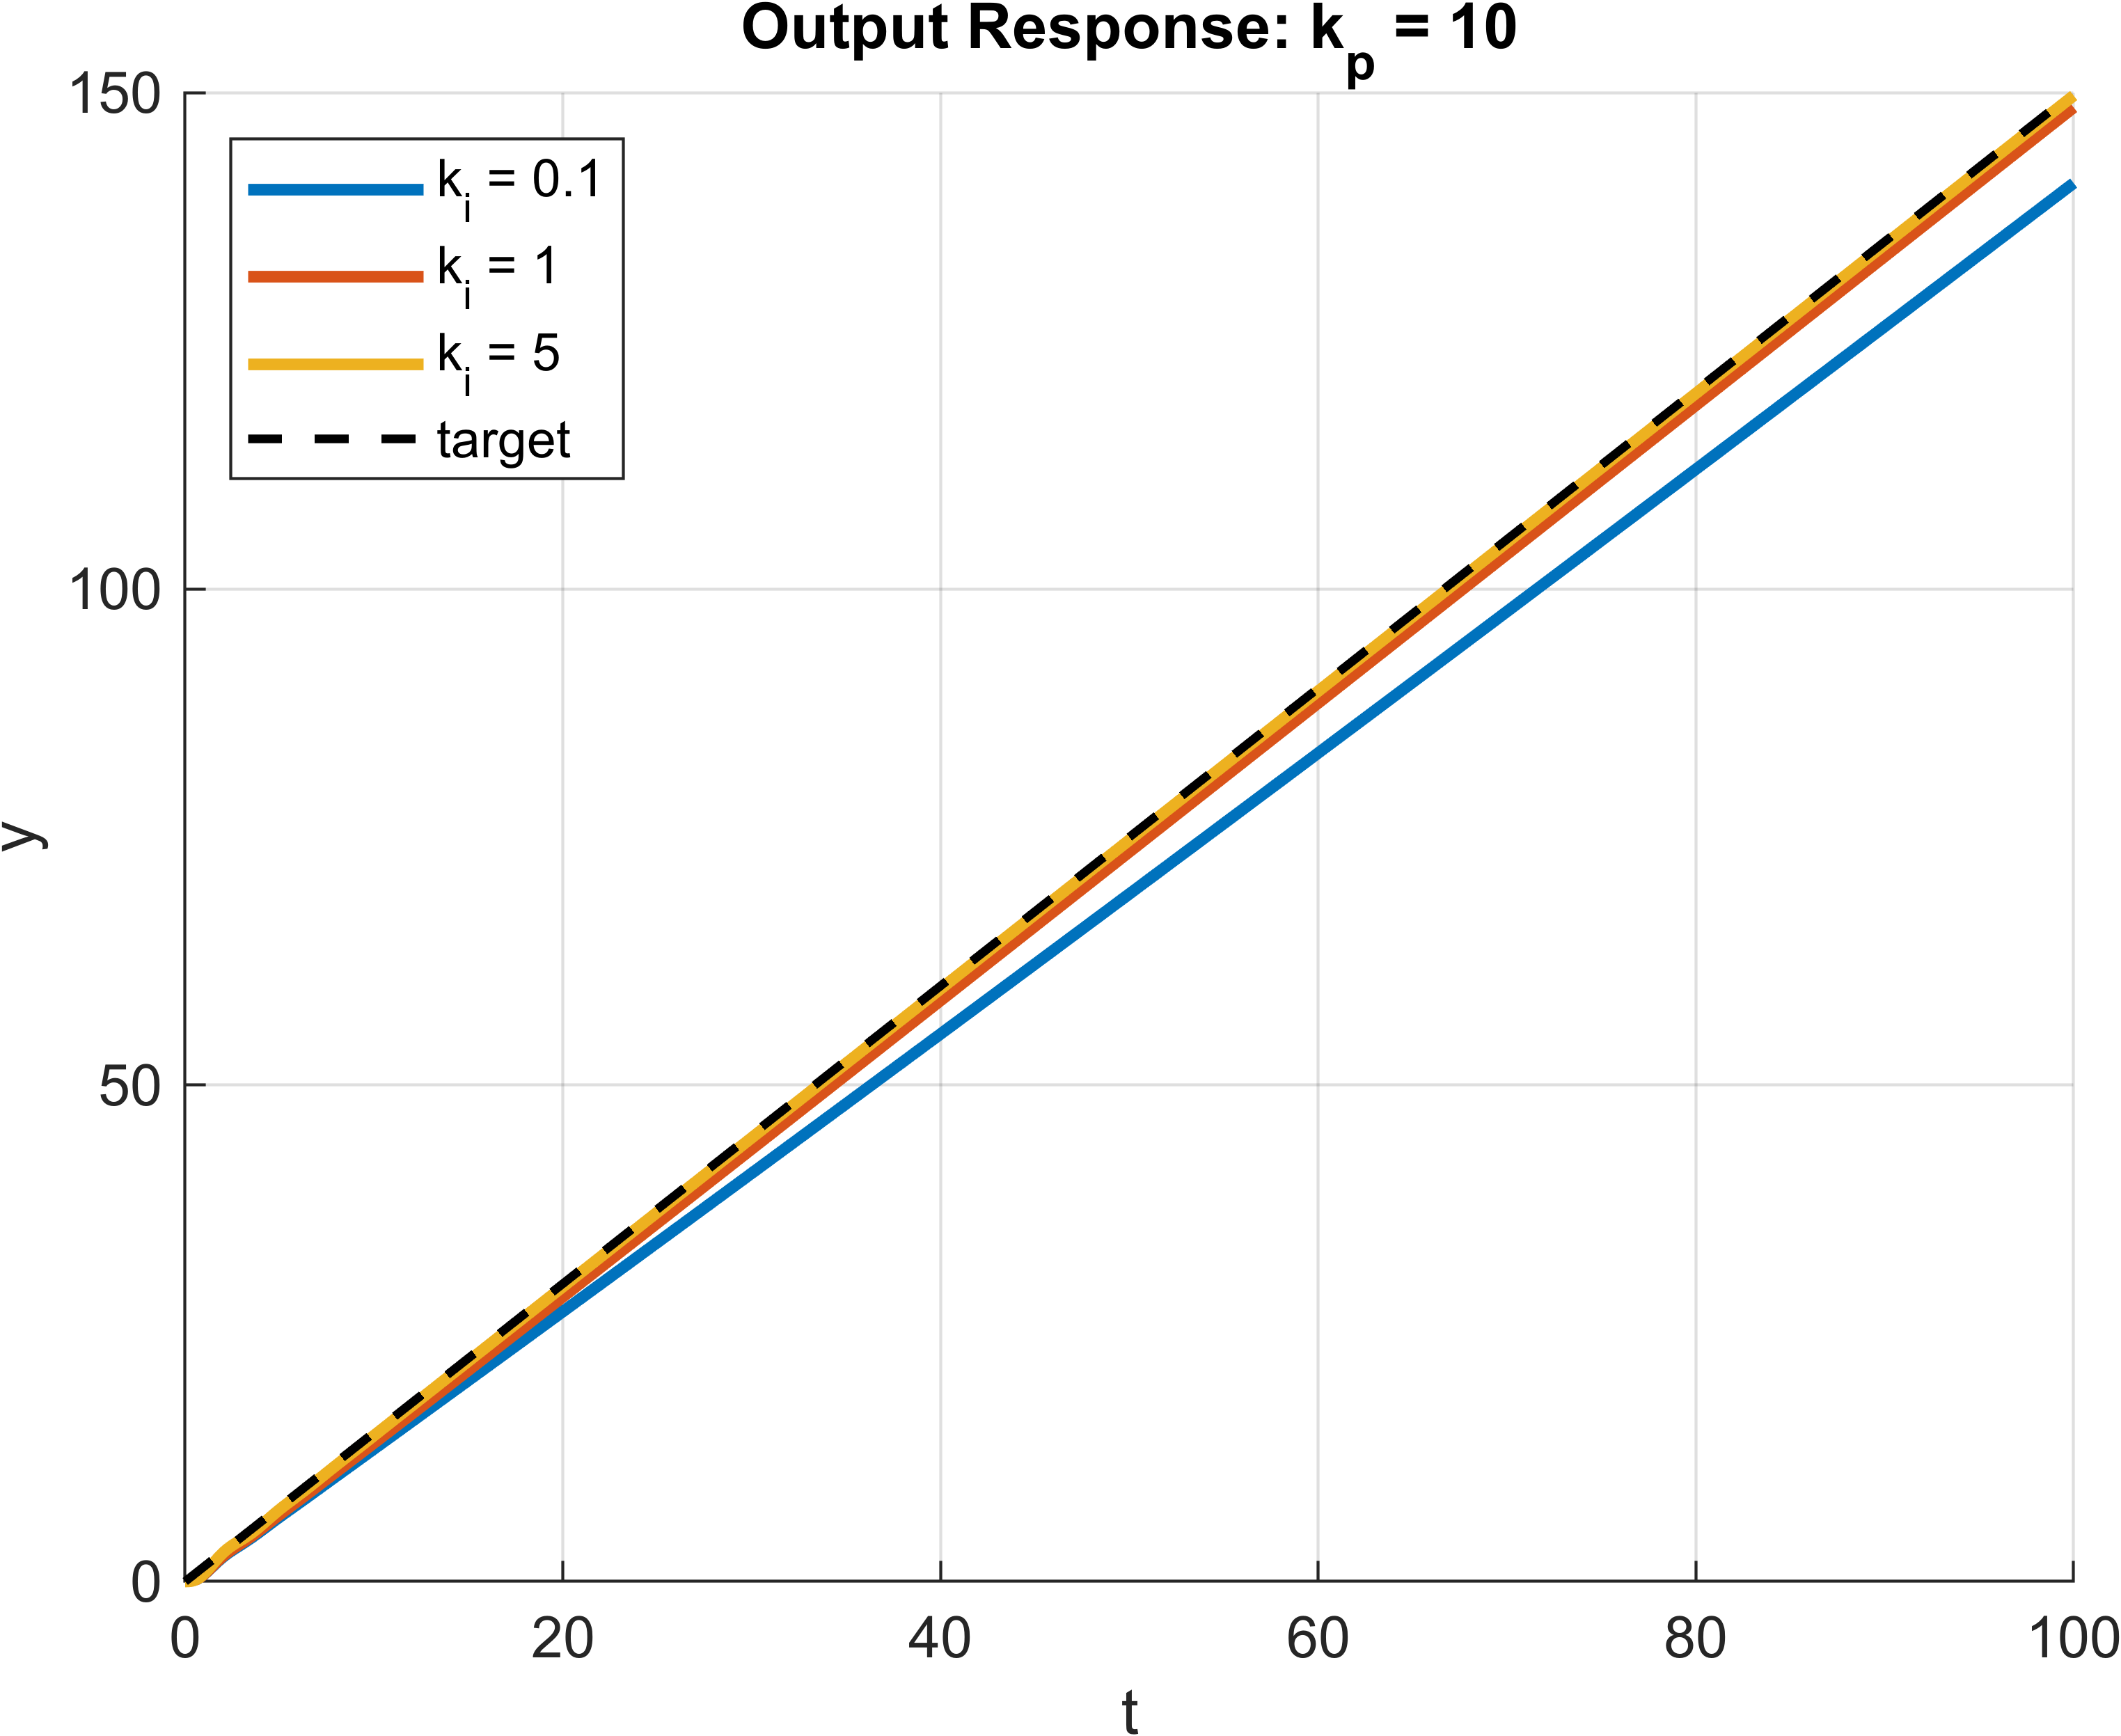
\includegraphics[width=1\textwidth, trim={1cm 0cm 1cm 0cm}]{../images/input_2_kp_10_output.png}
    \end{minipage}
    \hfill
    \begin{minipage}{0.45\textwidth}
        \centering
        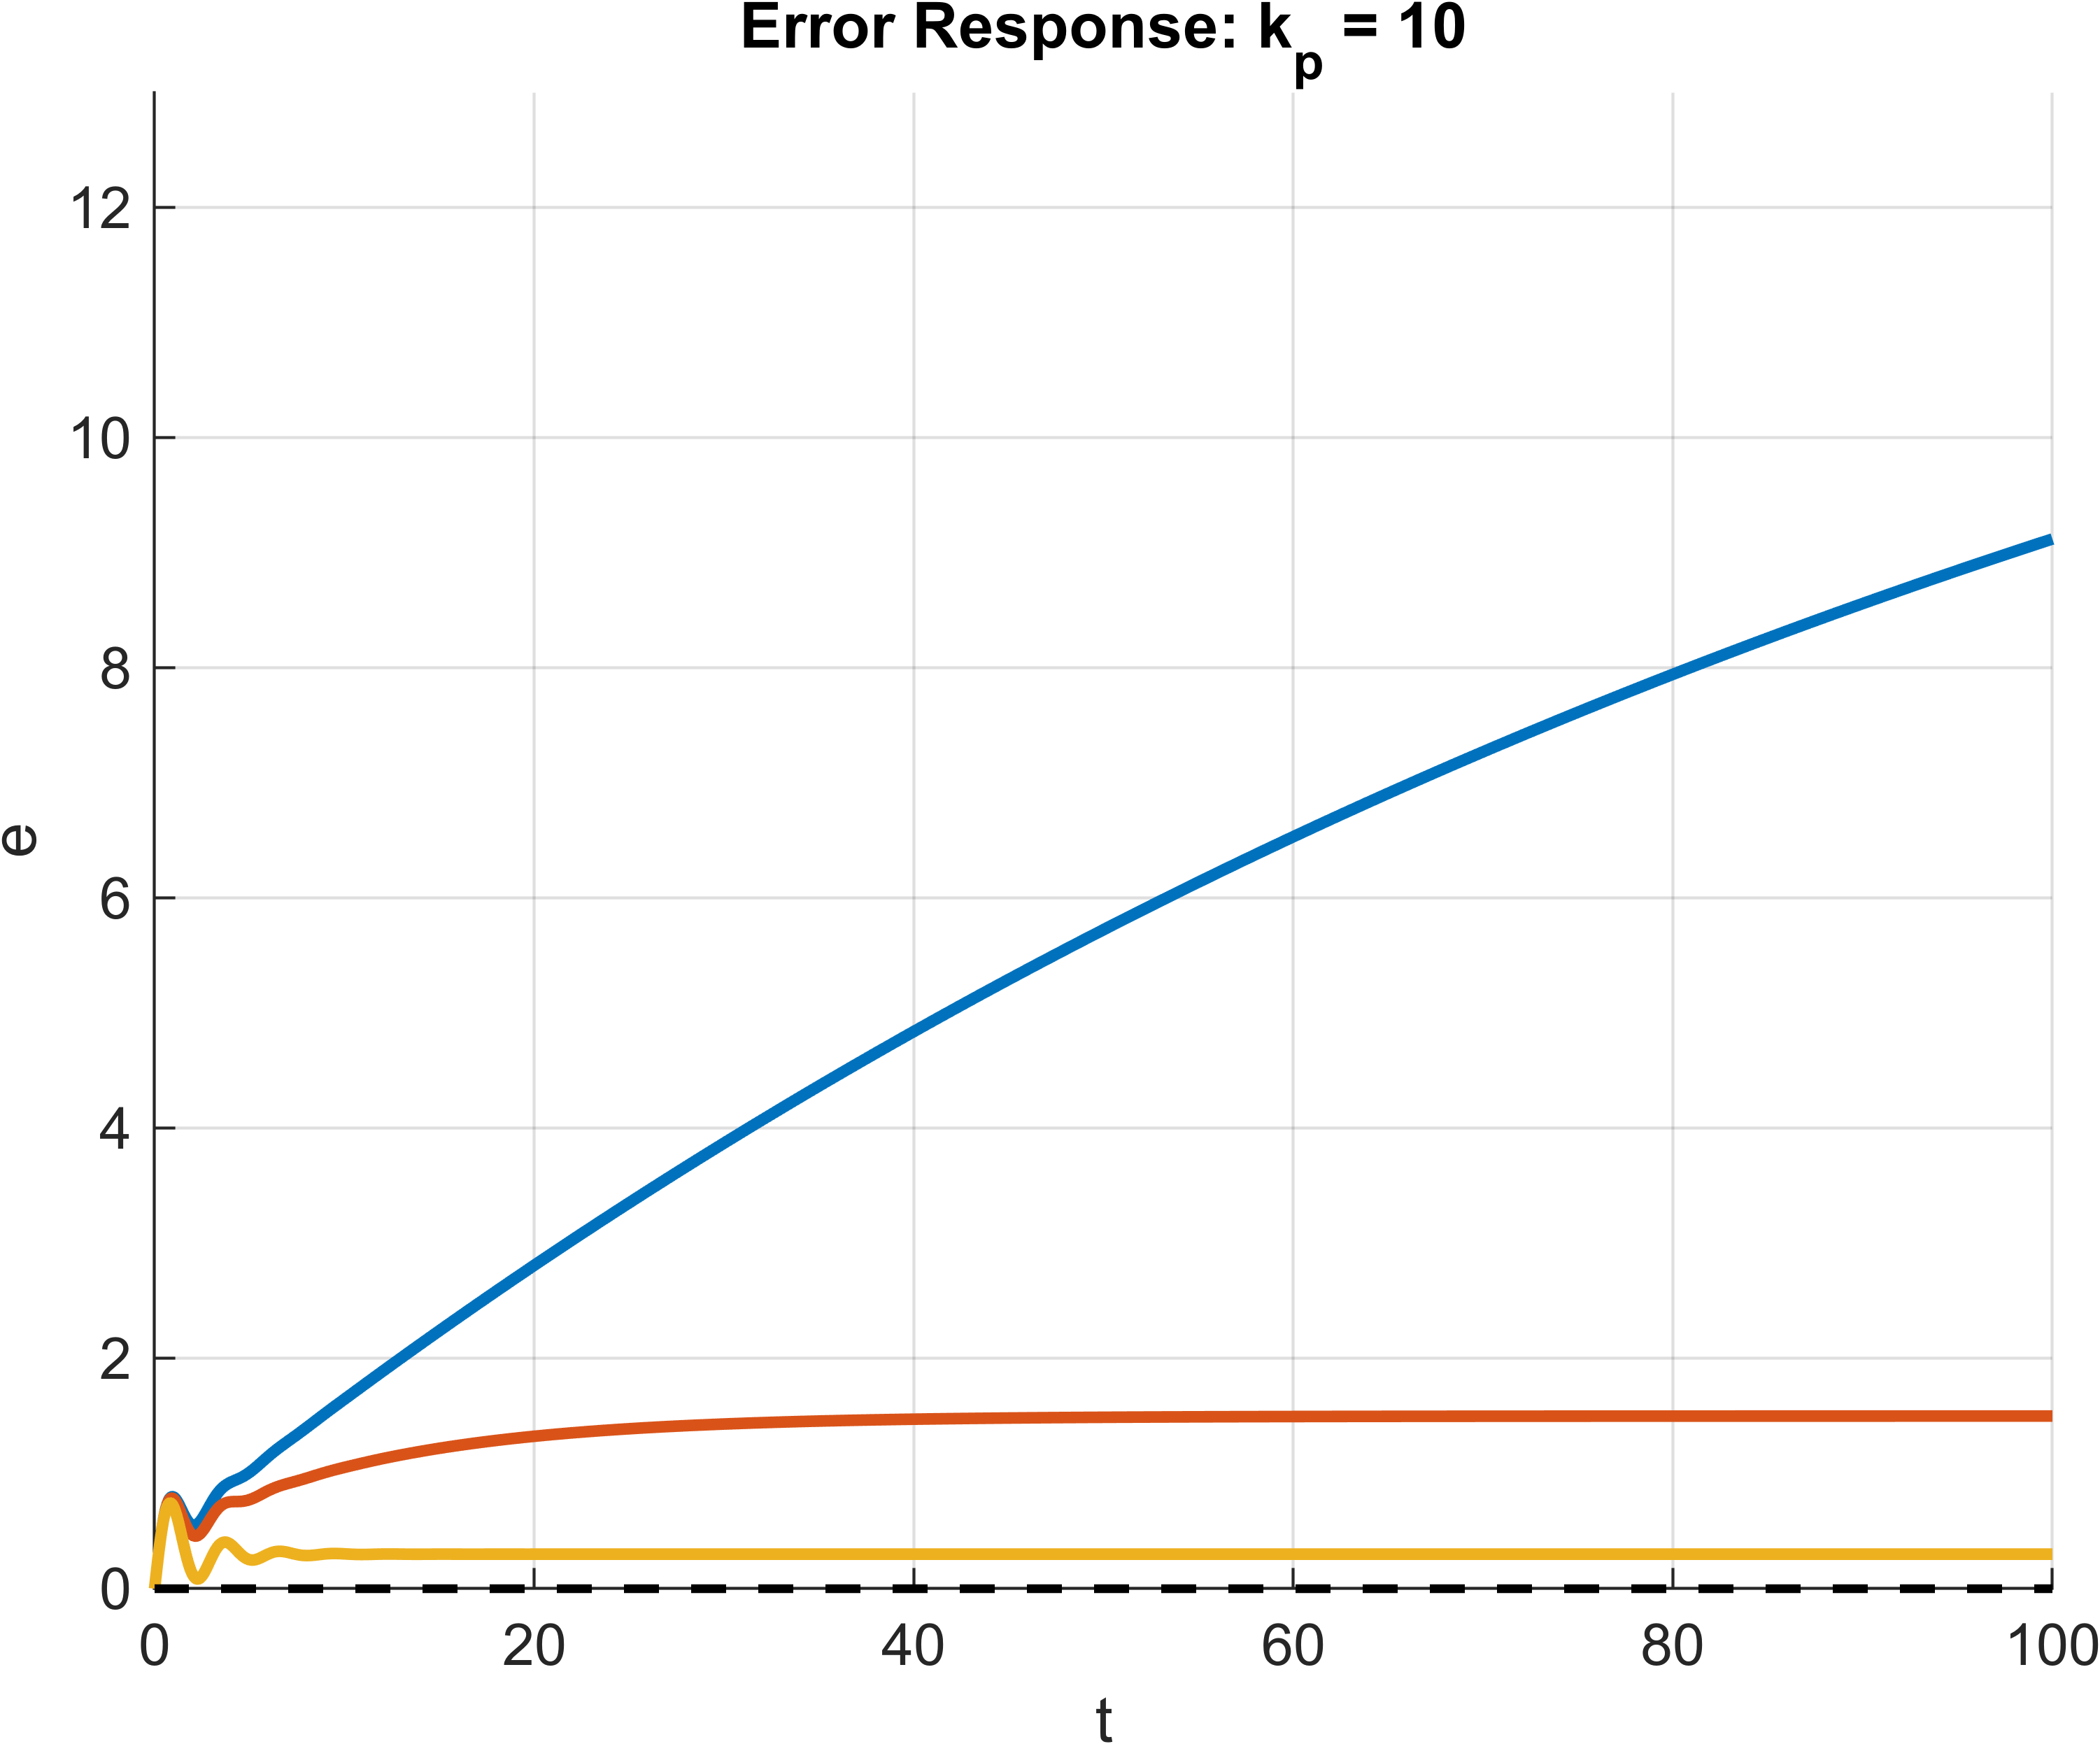
\includegraphics[width=1\textwidth, trim={1cm 0cm 1cm 0cm}]{../images/input_2_kp_10_error.png}
    \end{minipage}
    \caption{Графики $y(t)$ и $e(t)$ при $g(t) = 1.5t$ и $k_p = 10$}
\end{figure}
\begin{figure}[H]
    \centering
    \begin{minipage}{0.45\textwidth}
        \centering
        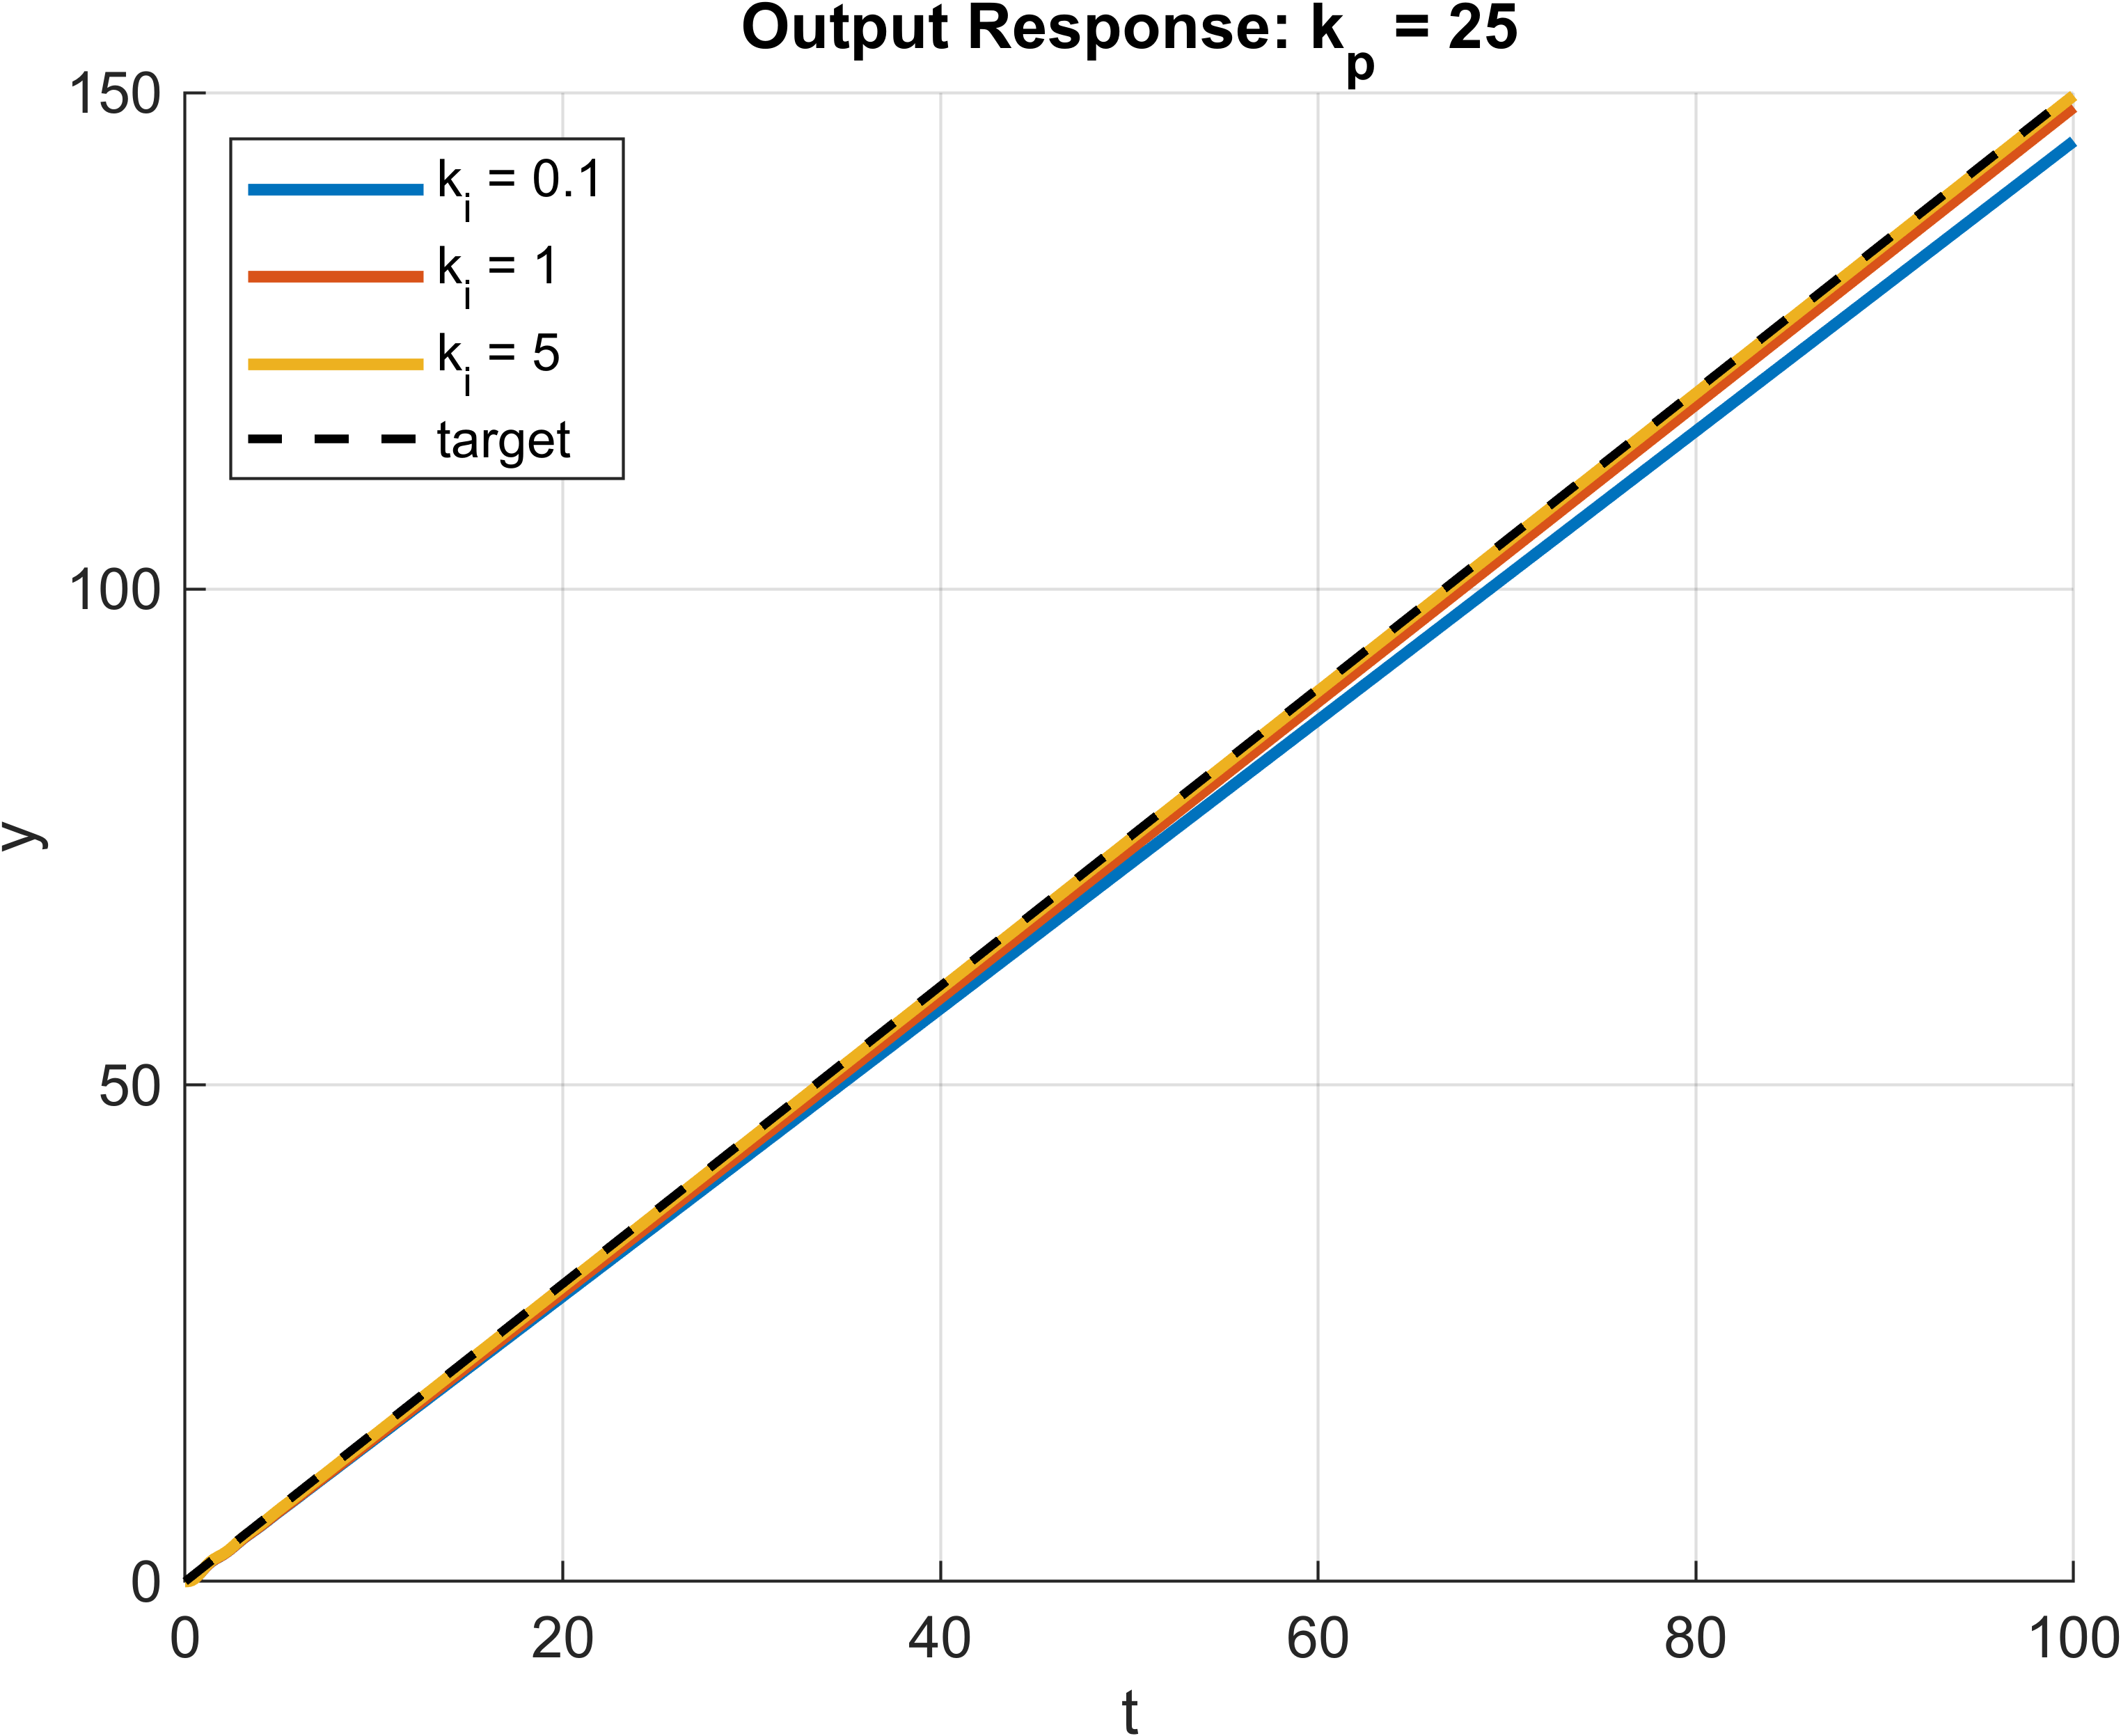
\includegraphics[width=1\textwidth, trim={1cm 0cm 1cm 0cm}]{../images/input_2_kp_25_output.png}
    \end{minipage}
    \hfill
    \begin{minipage}{0.45\textwidth}
        \centering
        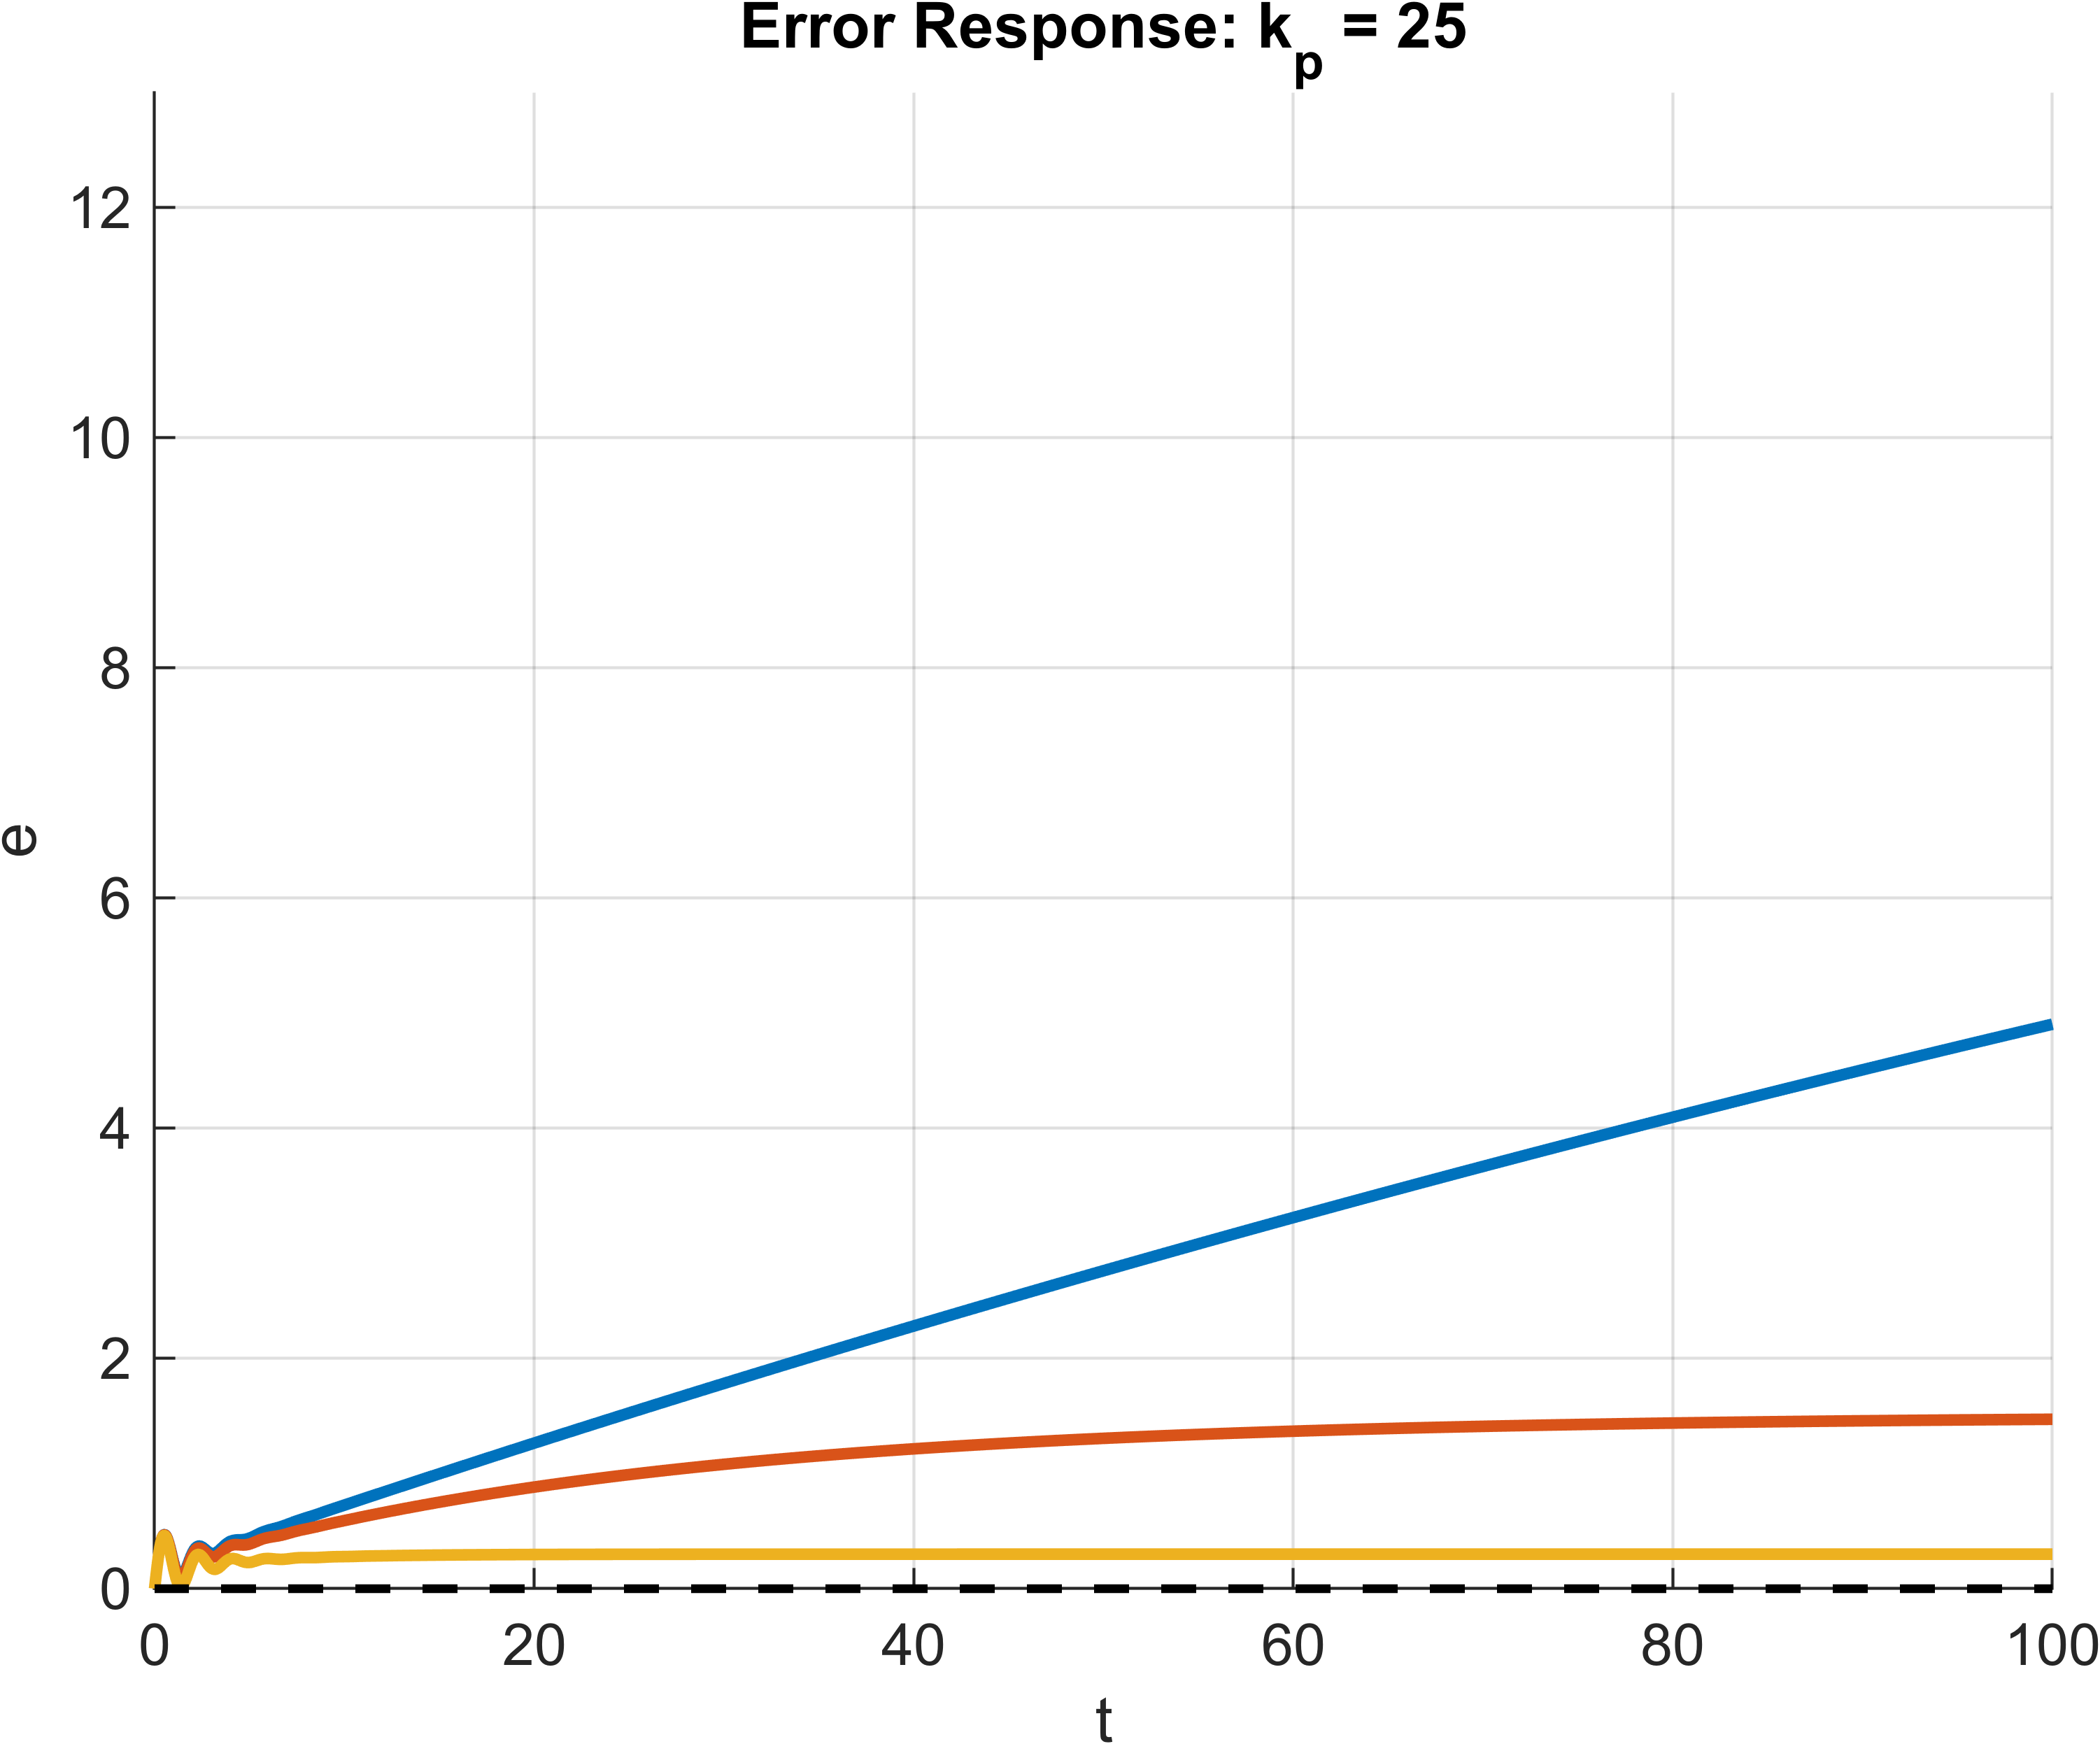
\includegraphics[width=1\textwidth, trim={1cm 0cm 1cm 0cm}]{../images/input_2_kp_25_error.png}
    \end{minipage}
    \caption{Графики $y(t)$ и $e(t)$ при $g(t) = 1.5t$ и $k_p = 25$}
\end{figure}

Аналитически определим предельное значение ошибки $e$ для каждой пары $k_p$ и $k_i$:
\[
    W_{g\to e} = \frac{1}{1 + (k_p+\frac{k_i}{s}) W(s)}
    = \frac{s}{s + (k_p+\frac{k_i}{s}) \frac{1}{2s^2 + 3s + 1}}
    = \frac{2s^3 + 3s^2 + s}{2s^3 + 3s^2 + s + k_p s + k_i}
\]
\[
    e_{\text{уст}} = \lim_{t \to \infty} e(t)
    = \lim_{s \to 0} s E(s)
    = \lim_{s \to 0} s W_{g\to e} G(s) =
\]\[
    = \lim_{s \to 0} s \frac{2s^3 + 3s^2 + s}{2s^3 + 3s^2 + s + k_p s + k_i} \frac{1.5}{s^2}
    = \frac{1.5}{k_i}
\]
\[
    k_i = 0.1, \, k_p = 5,\, 10,\, 25: e_{\text{уст}} = 15
\]
\[
    k_i = 1, \, k_p = 5,\, 10,\, 25: e_{\text{уст}} = 1.5
\]
\[
    k_i = 5, \, k_p = 5,\, 10,\, 25: e_{\text{уст}} = 0.3
\]

Из графиков и аналитических расчетов видно, что ПИ-регулятор 
обеспечивает постоянную установившуюся ошибку. При этом она 
зависит от $k_i$ и не зависит от $k_p$.

\section{Режим слежения за гармоническим сигналом при $g(t) = a\sin(\omega t)$}
Выполним моделирование:
\begin{figure}[H]
    \centering
    \begin{minipage}{0.45\textwidth}
        \centering
        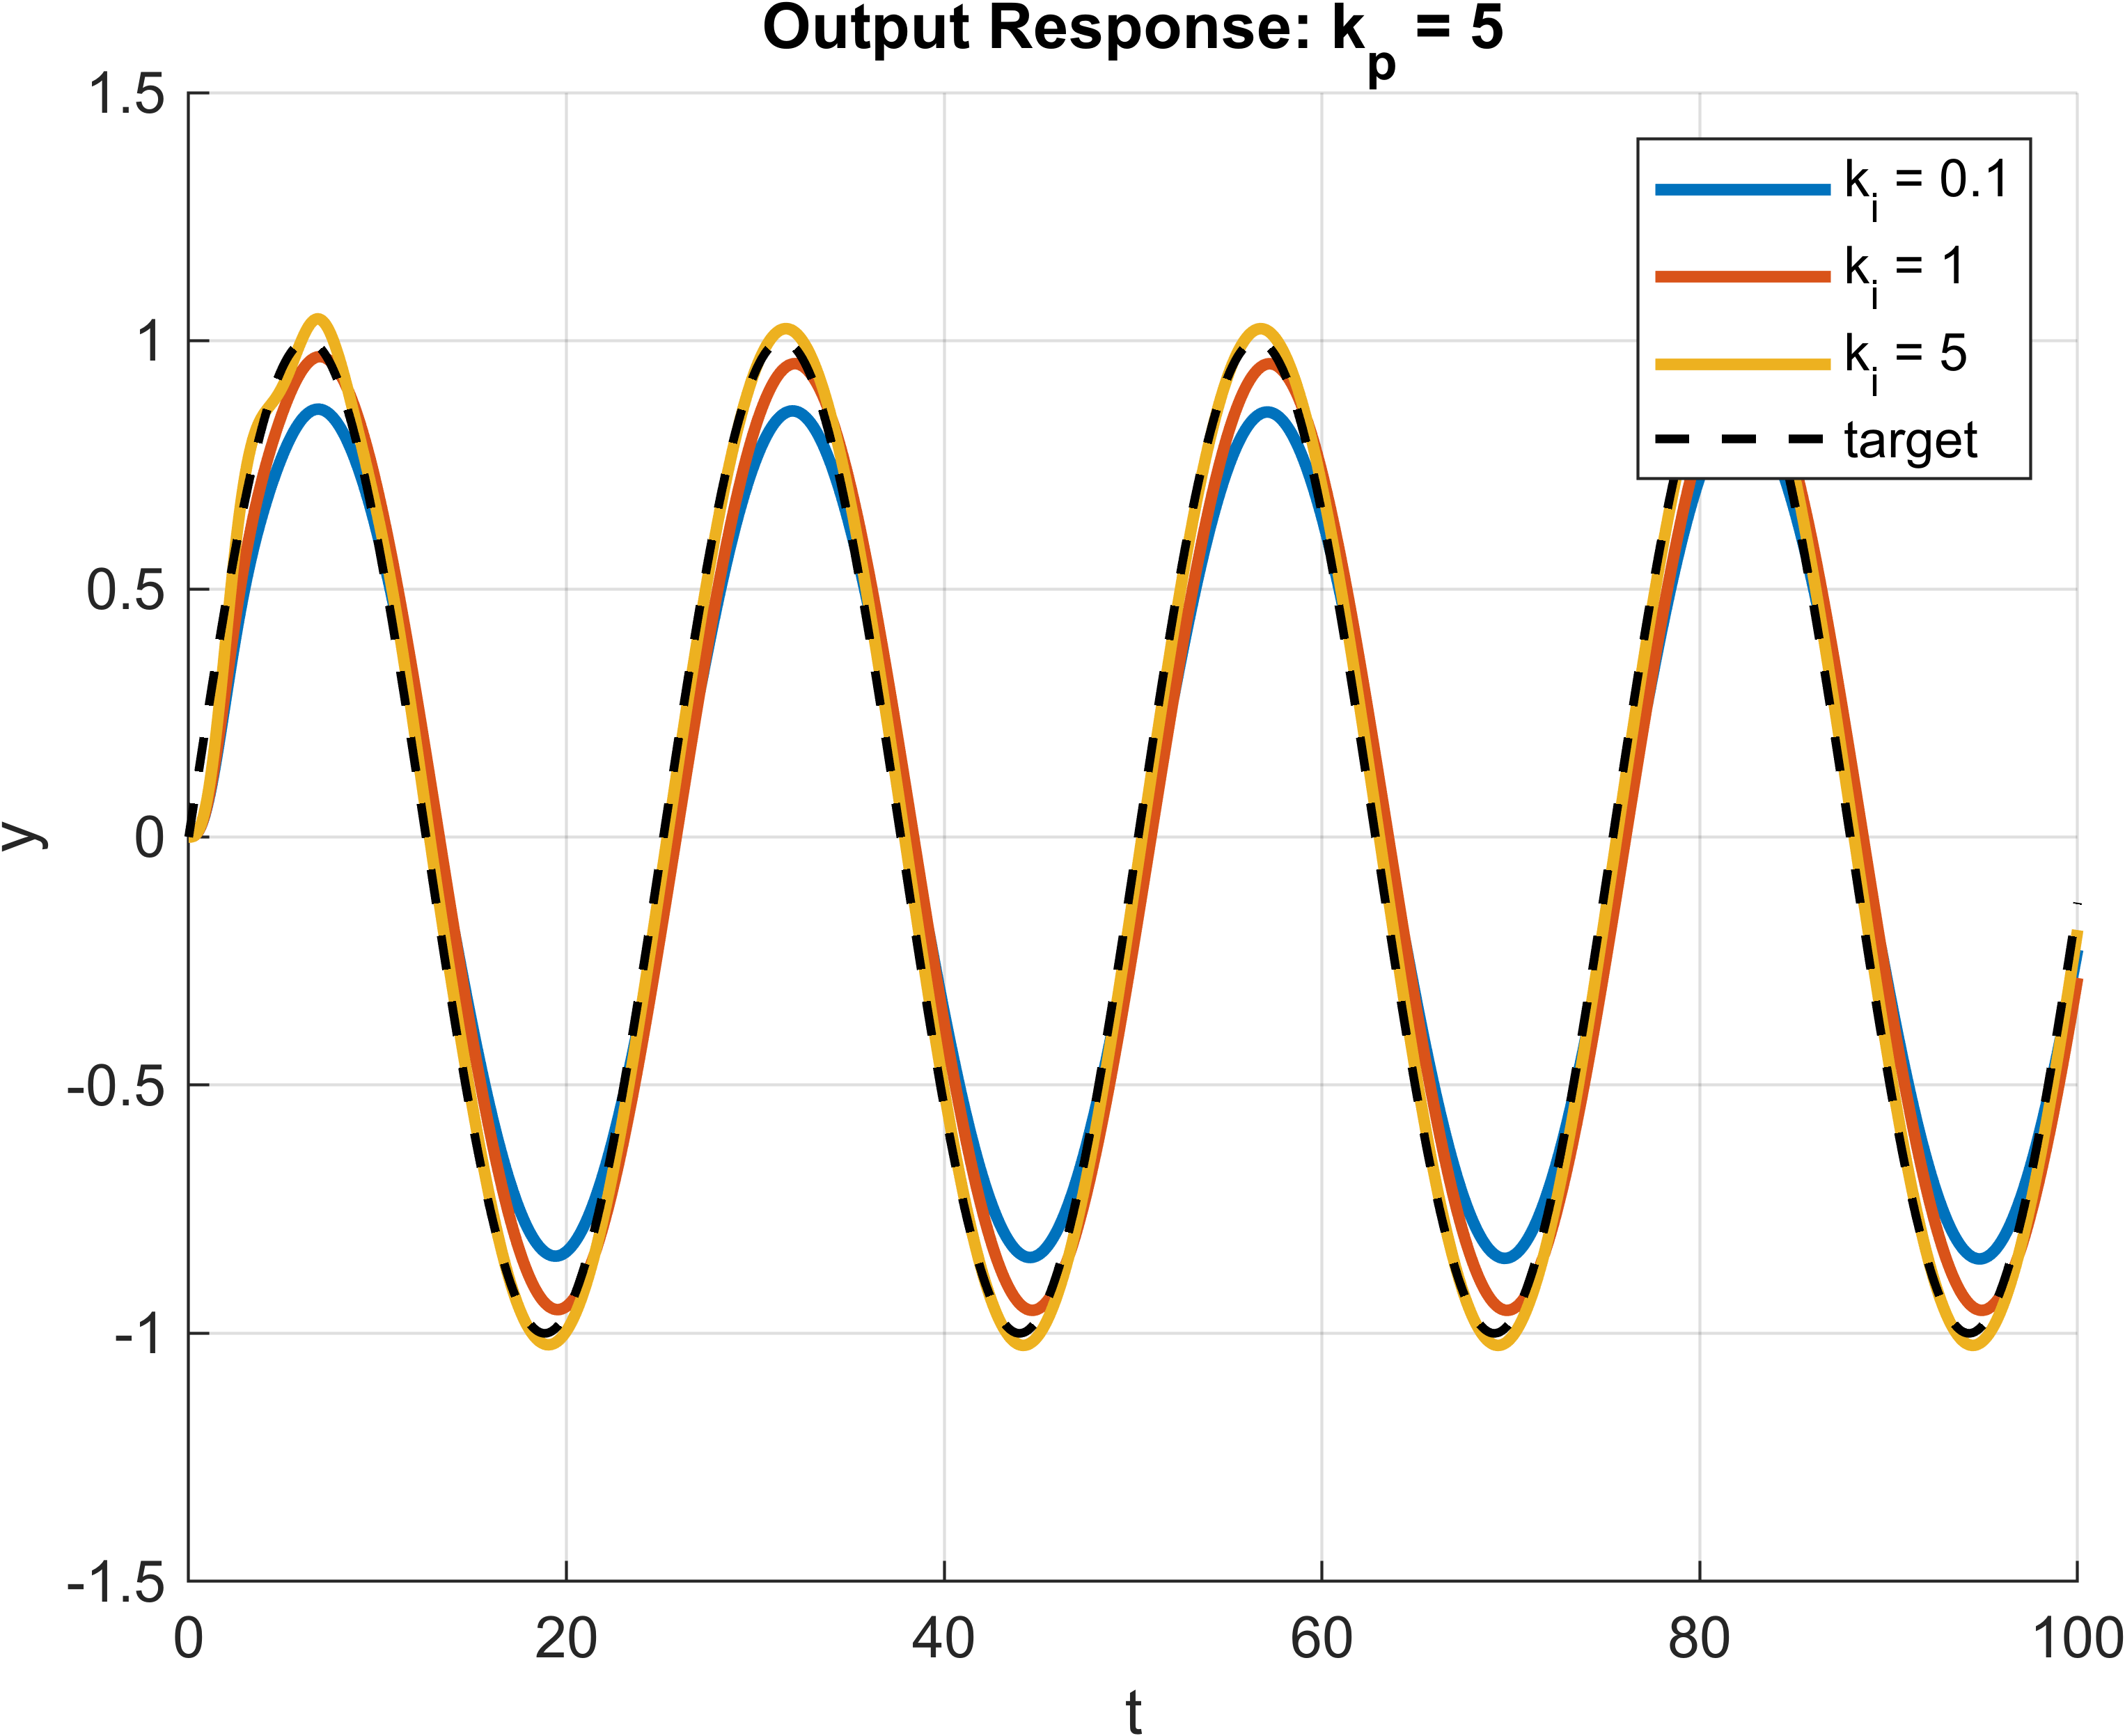
\includegraphics[width=1\textwidth, trim={1cm 0cm 1cm 0cm}]{../images/input_4_kp_5_output.png}
    \end{minipage}
    \hfill
    \begin{minipage}{0.45\textwidth}
        \centering
        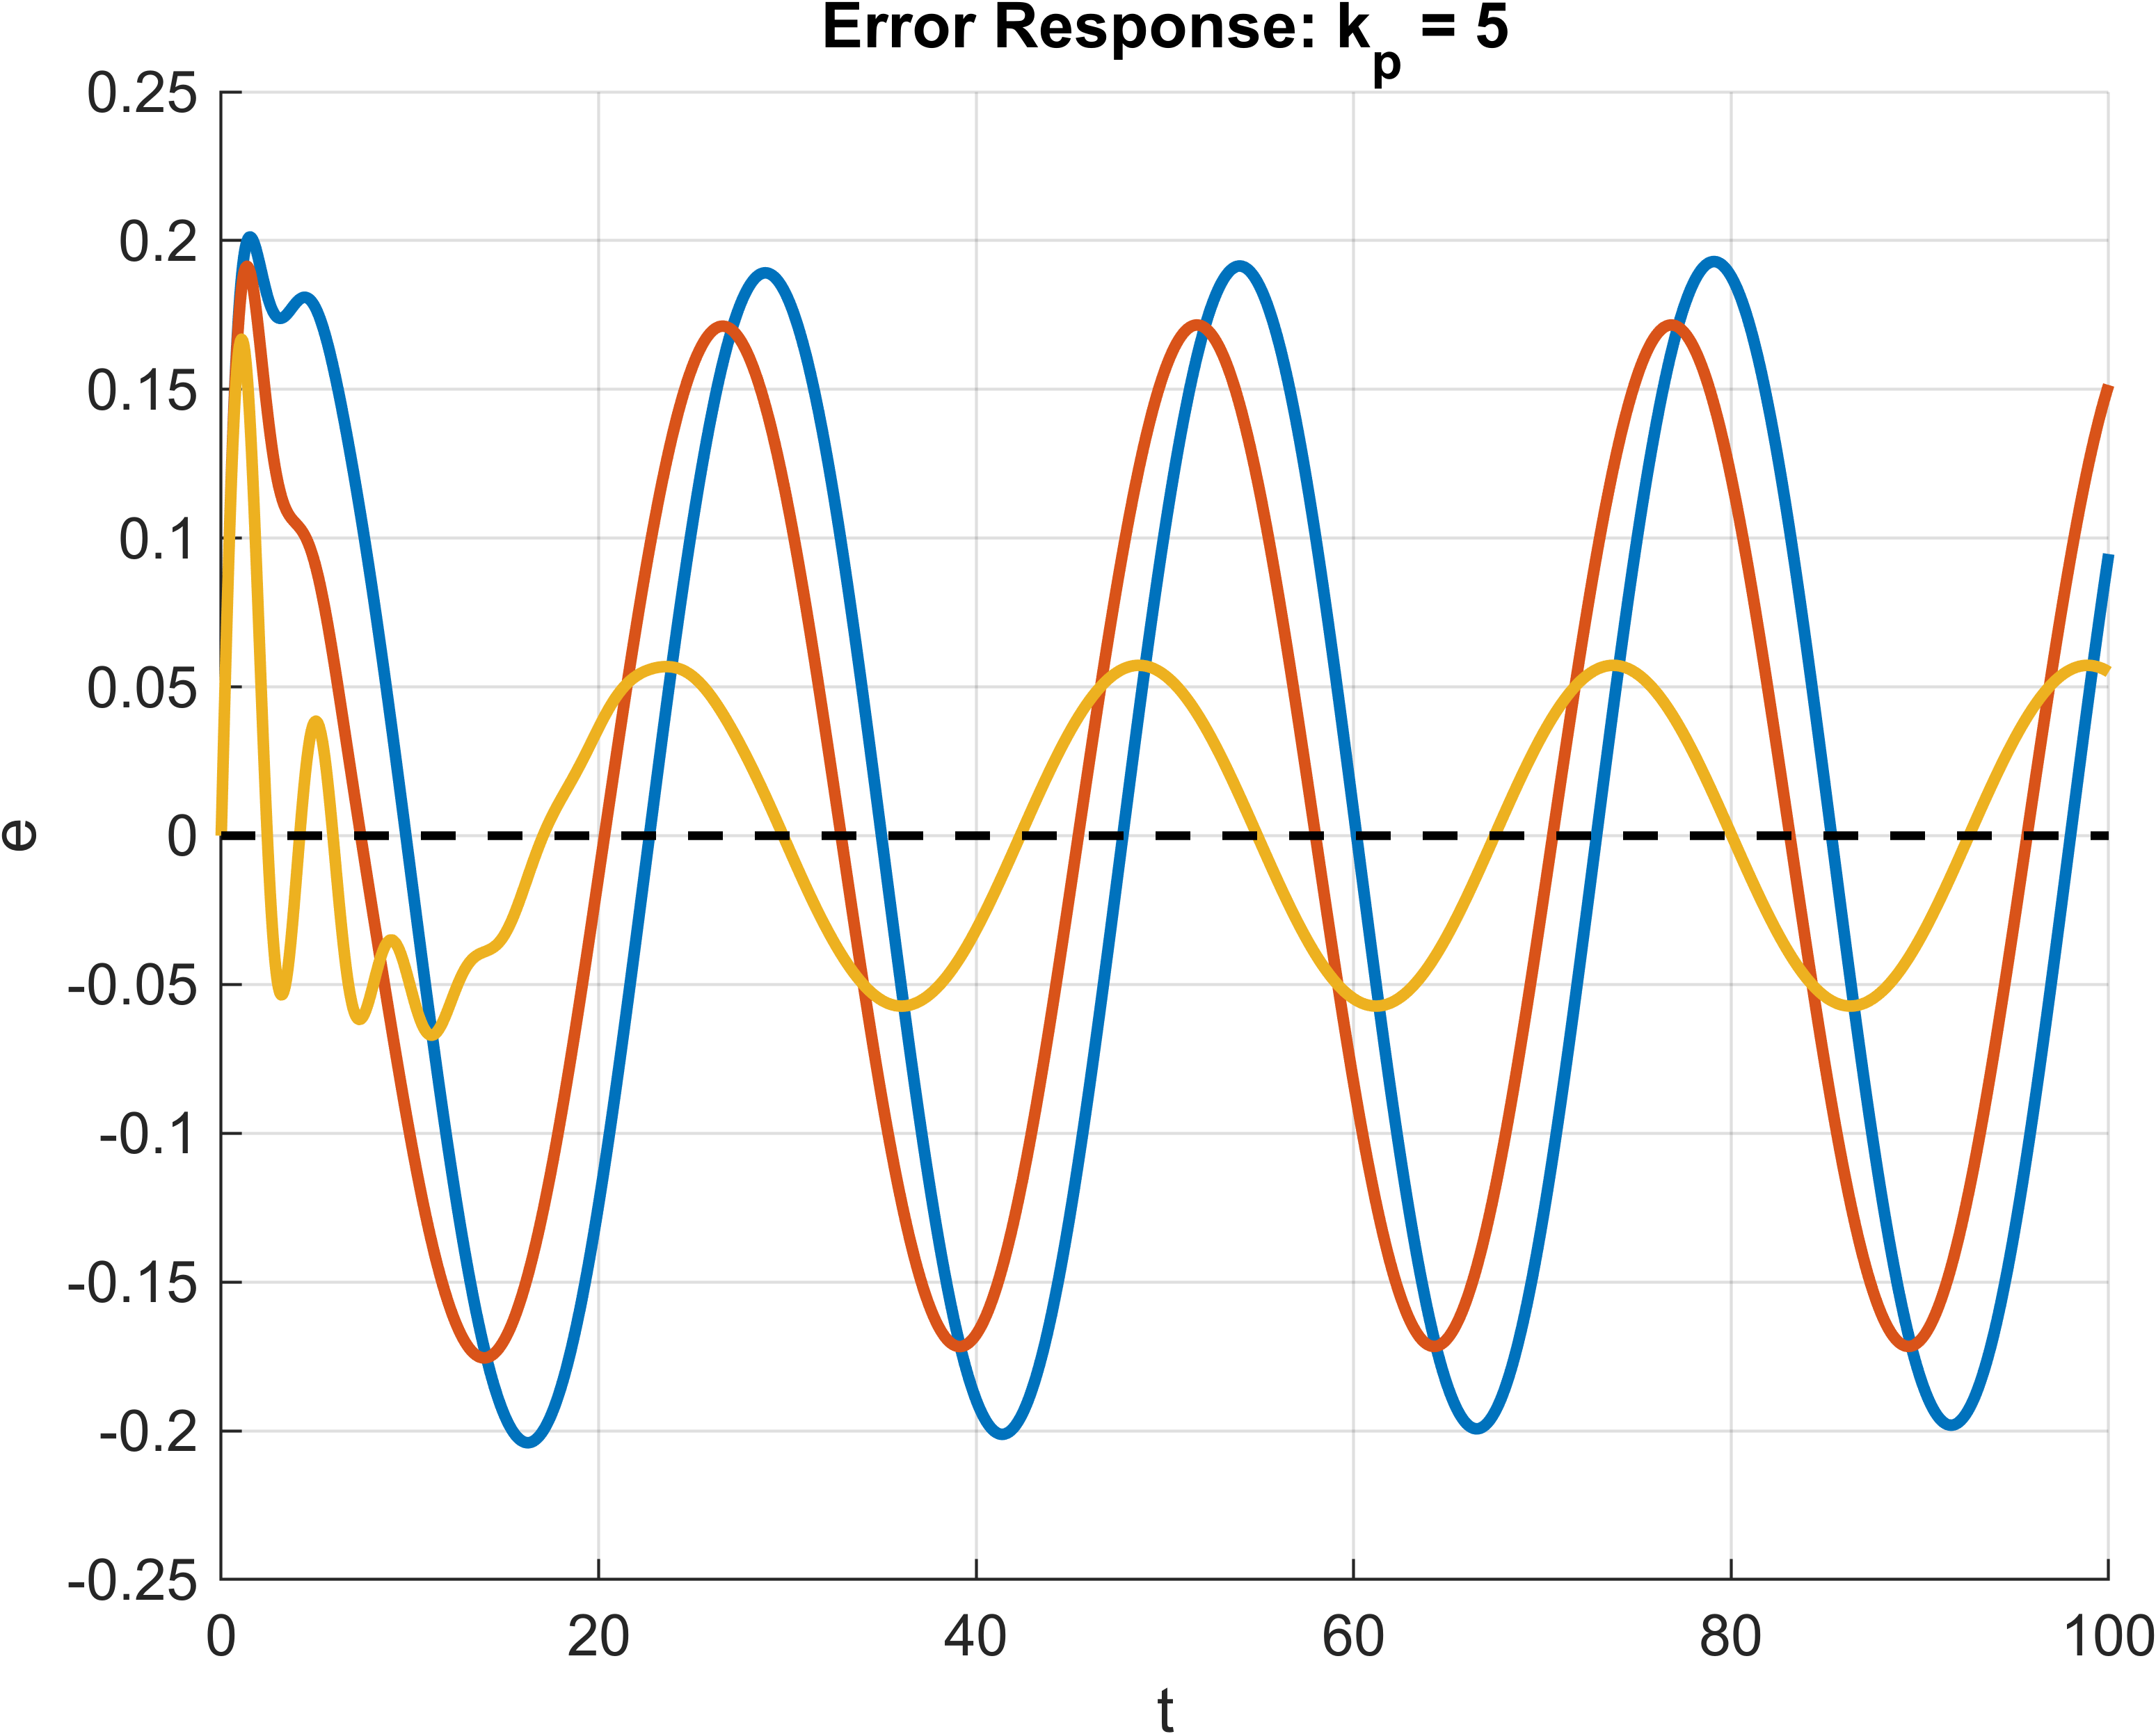
\includegraphics[width=1\textwidth, trim={1cm 0cm 1cm 0cm}]{../images/input_4_kp_5_error.png}
    \end{minipage}
    \caption{Графики $y(t)$ и $e(t)$ при $g(t) = \sin(0.25t)$ и $k_p = 5$}
\end{figure}
\begin{figure}[H]
    \centering
    \begin{minipage}{0.45\textwidth}
        \centering
        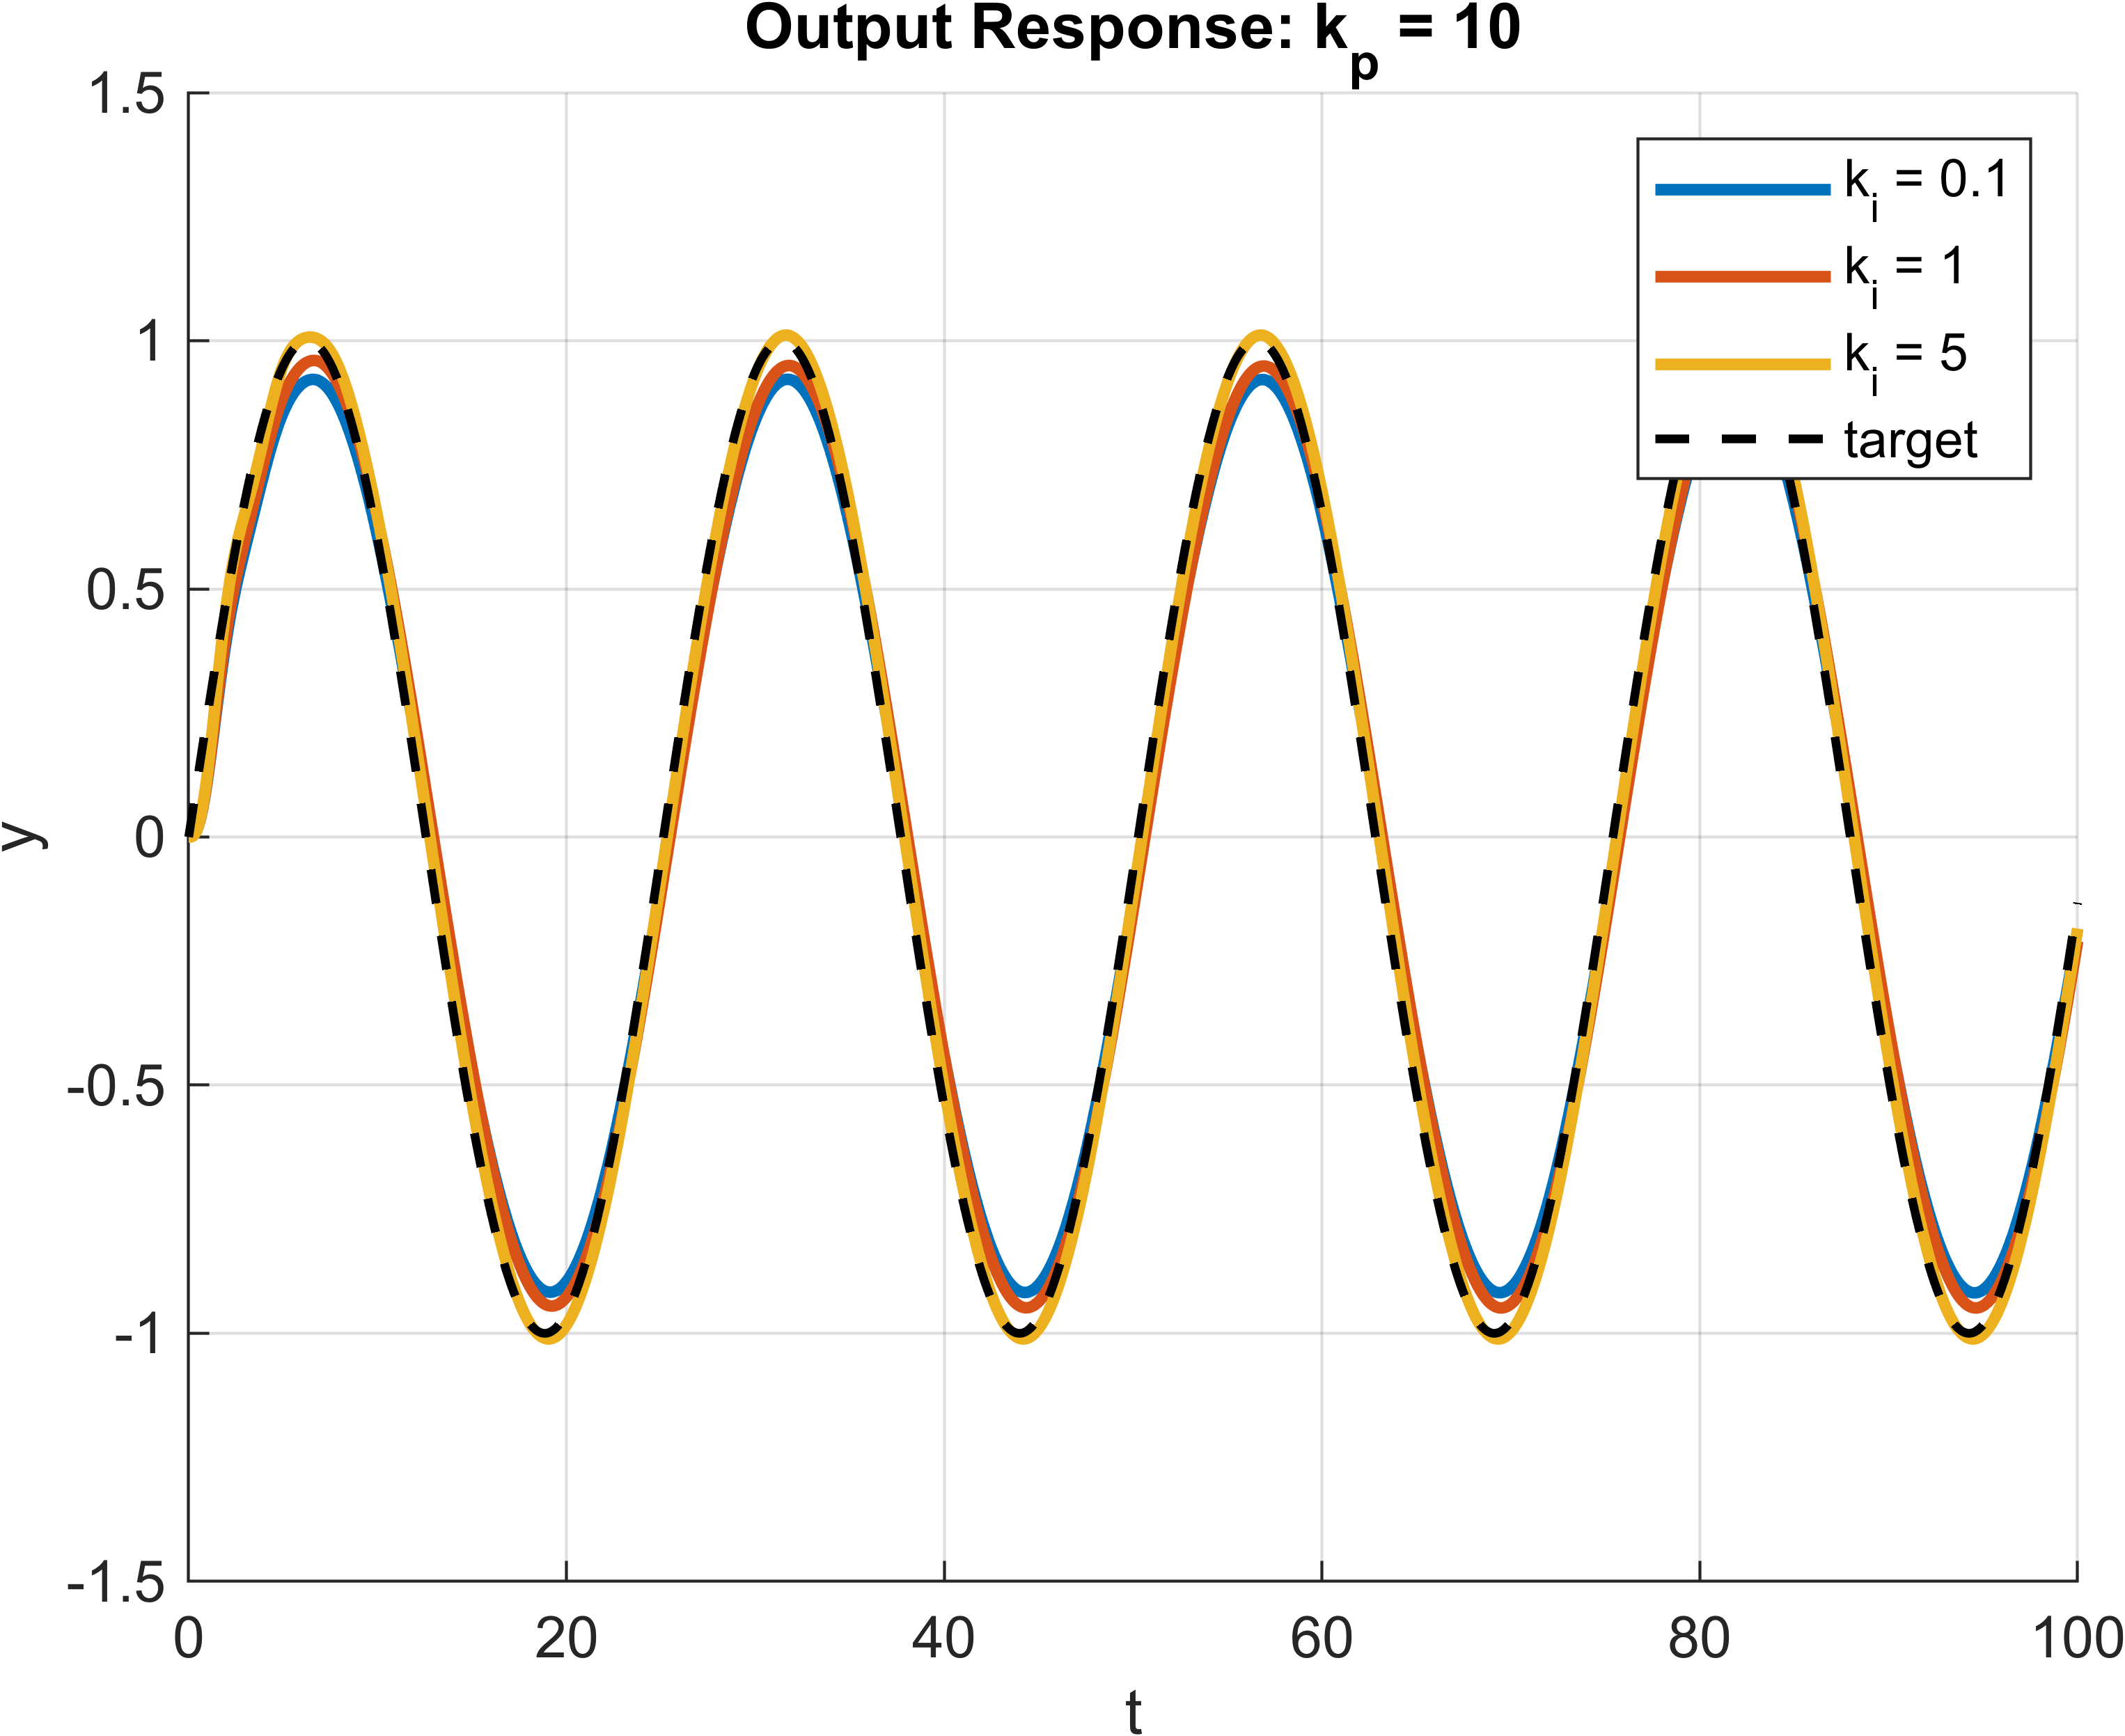
\includegraphics[width=1\textwidth, trim={1cm 0cm 1cm 0cm}]{../images/input_4_kp_10_output.png}
    \end{minipage}
    \hfill
    \begin{minipage}{0.45\textwidth}
        \centering
        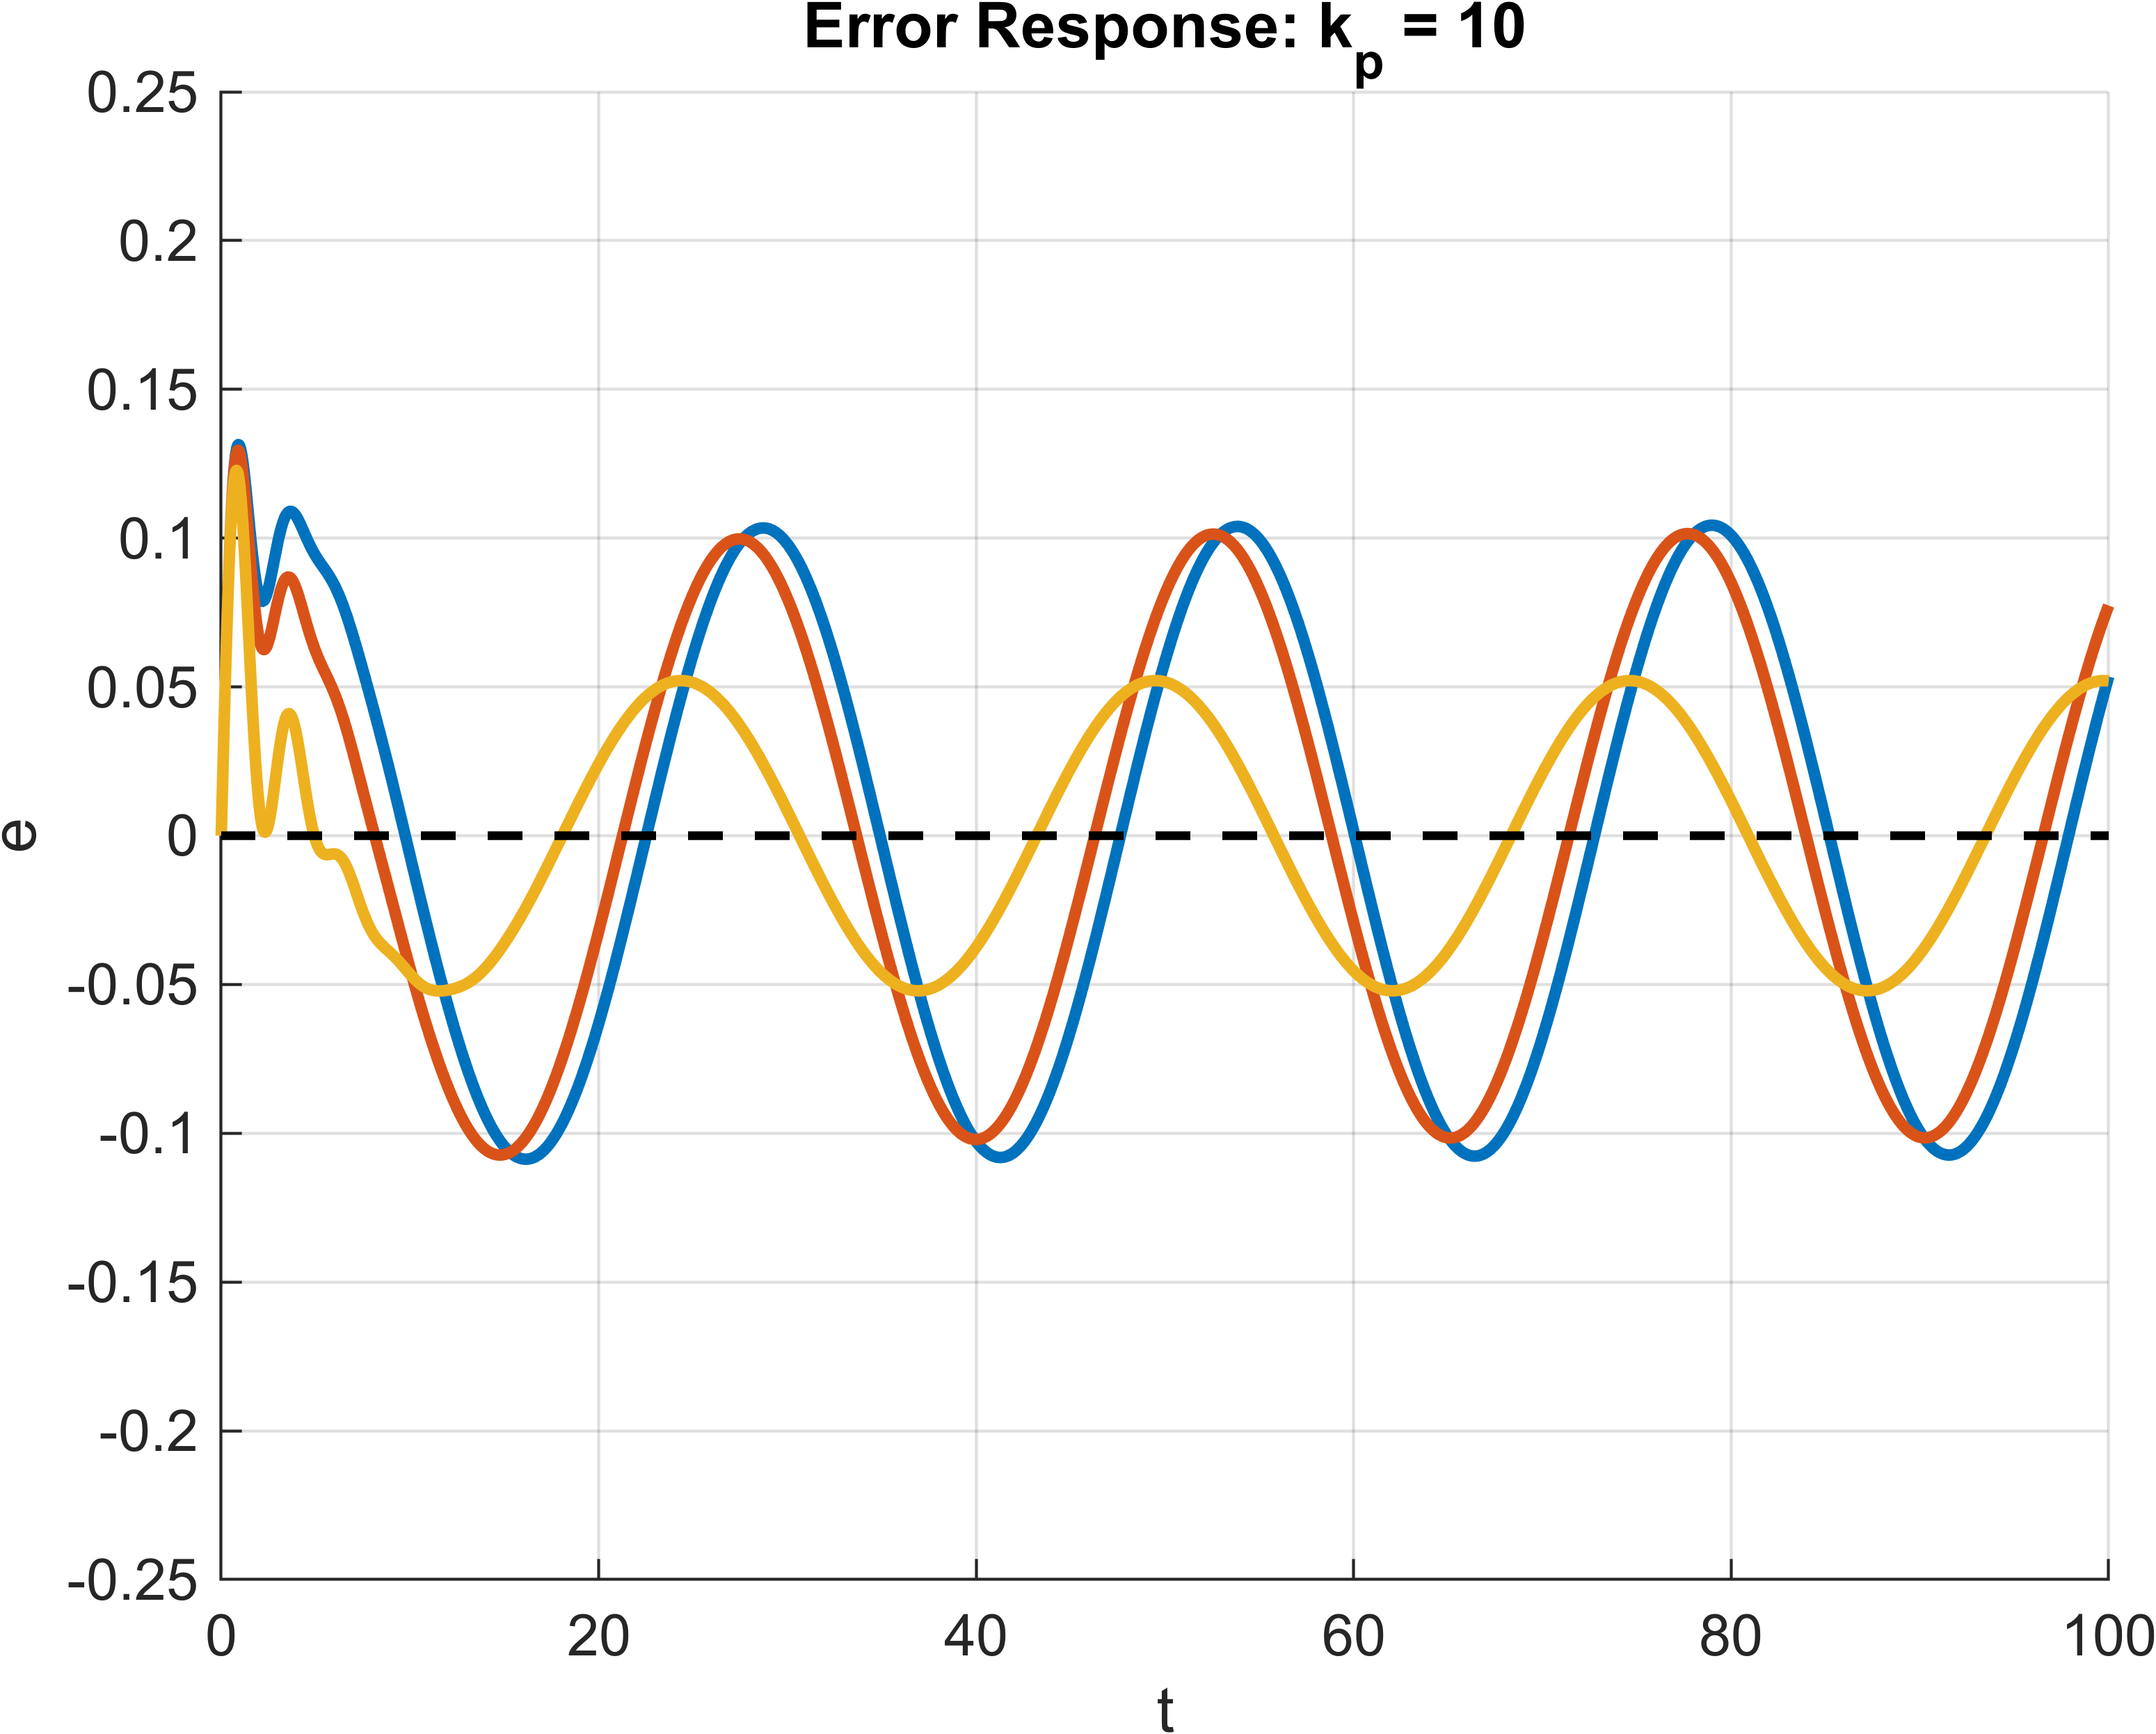
\includegraphics[width=1\textwidth, trim={1cm 0cm 1cm 0cm}]{../images/input_4_kp_10_error.png}
    \end{minipage}
    \caption{Графики $y(t)$ и $e(t)$ при $g(t) = \sin(0.25t)$ и $k_p = 10$}
\end{figure}
\begin{figure}[H]
    \centering
    \begin{minipage}{0.45\textwidth}
        \centering
        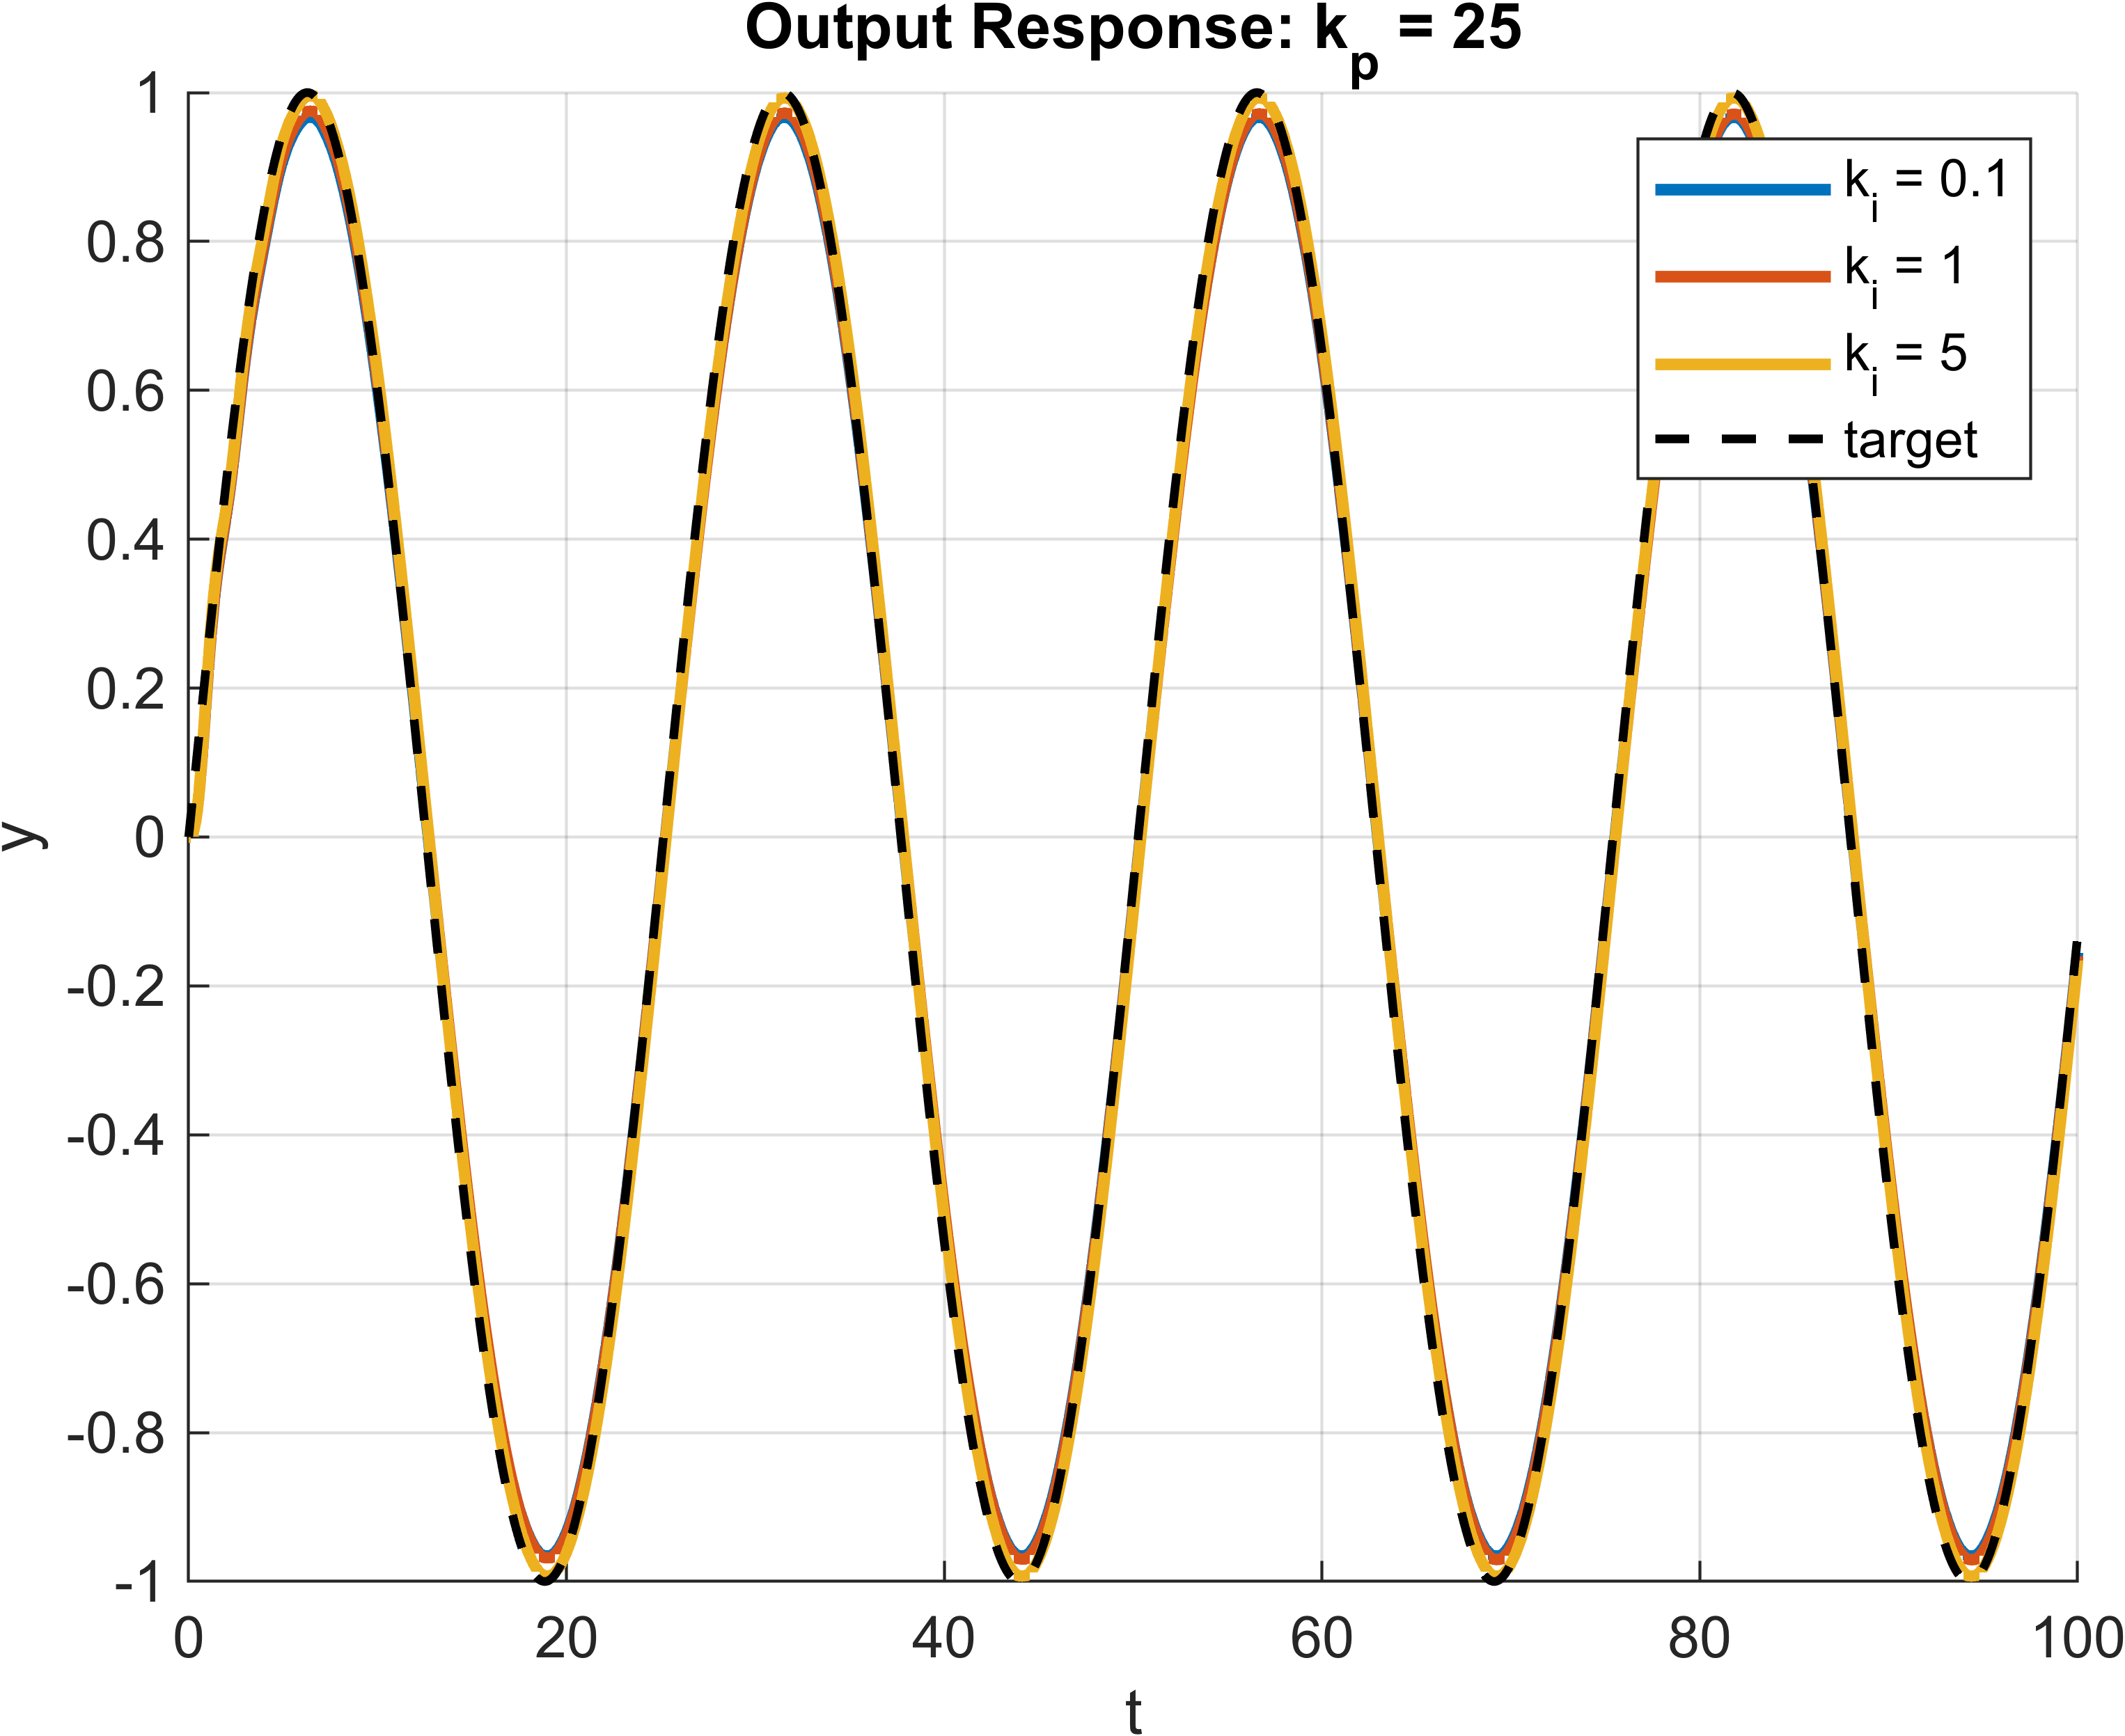
\includegraphics[width=1\textwidth, trim={1cm 0cm 1cm 0cm}]{../images/input_4_kp_25_output.png}
    \end{minipage}
    \hfill
    \begin{minipage}{0.45\textwidth}
        \centering
        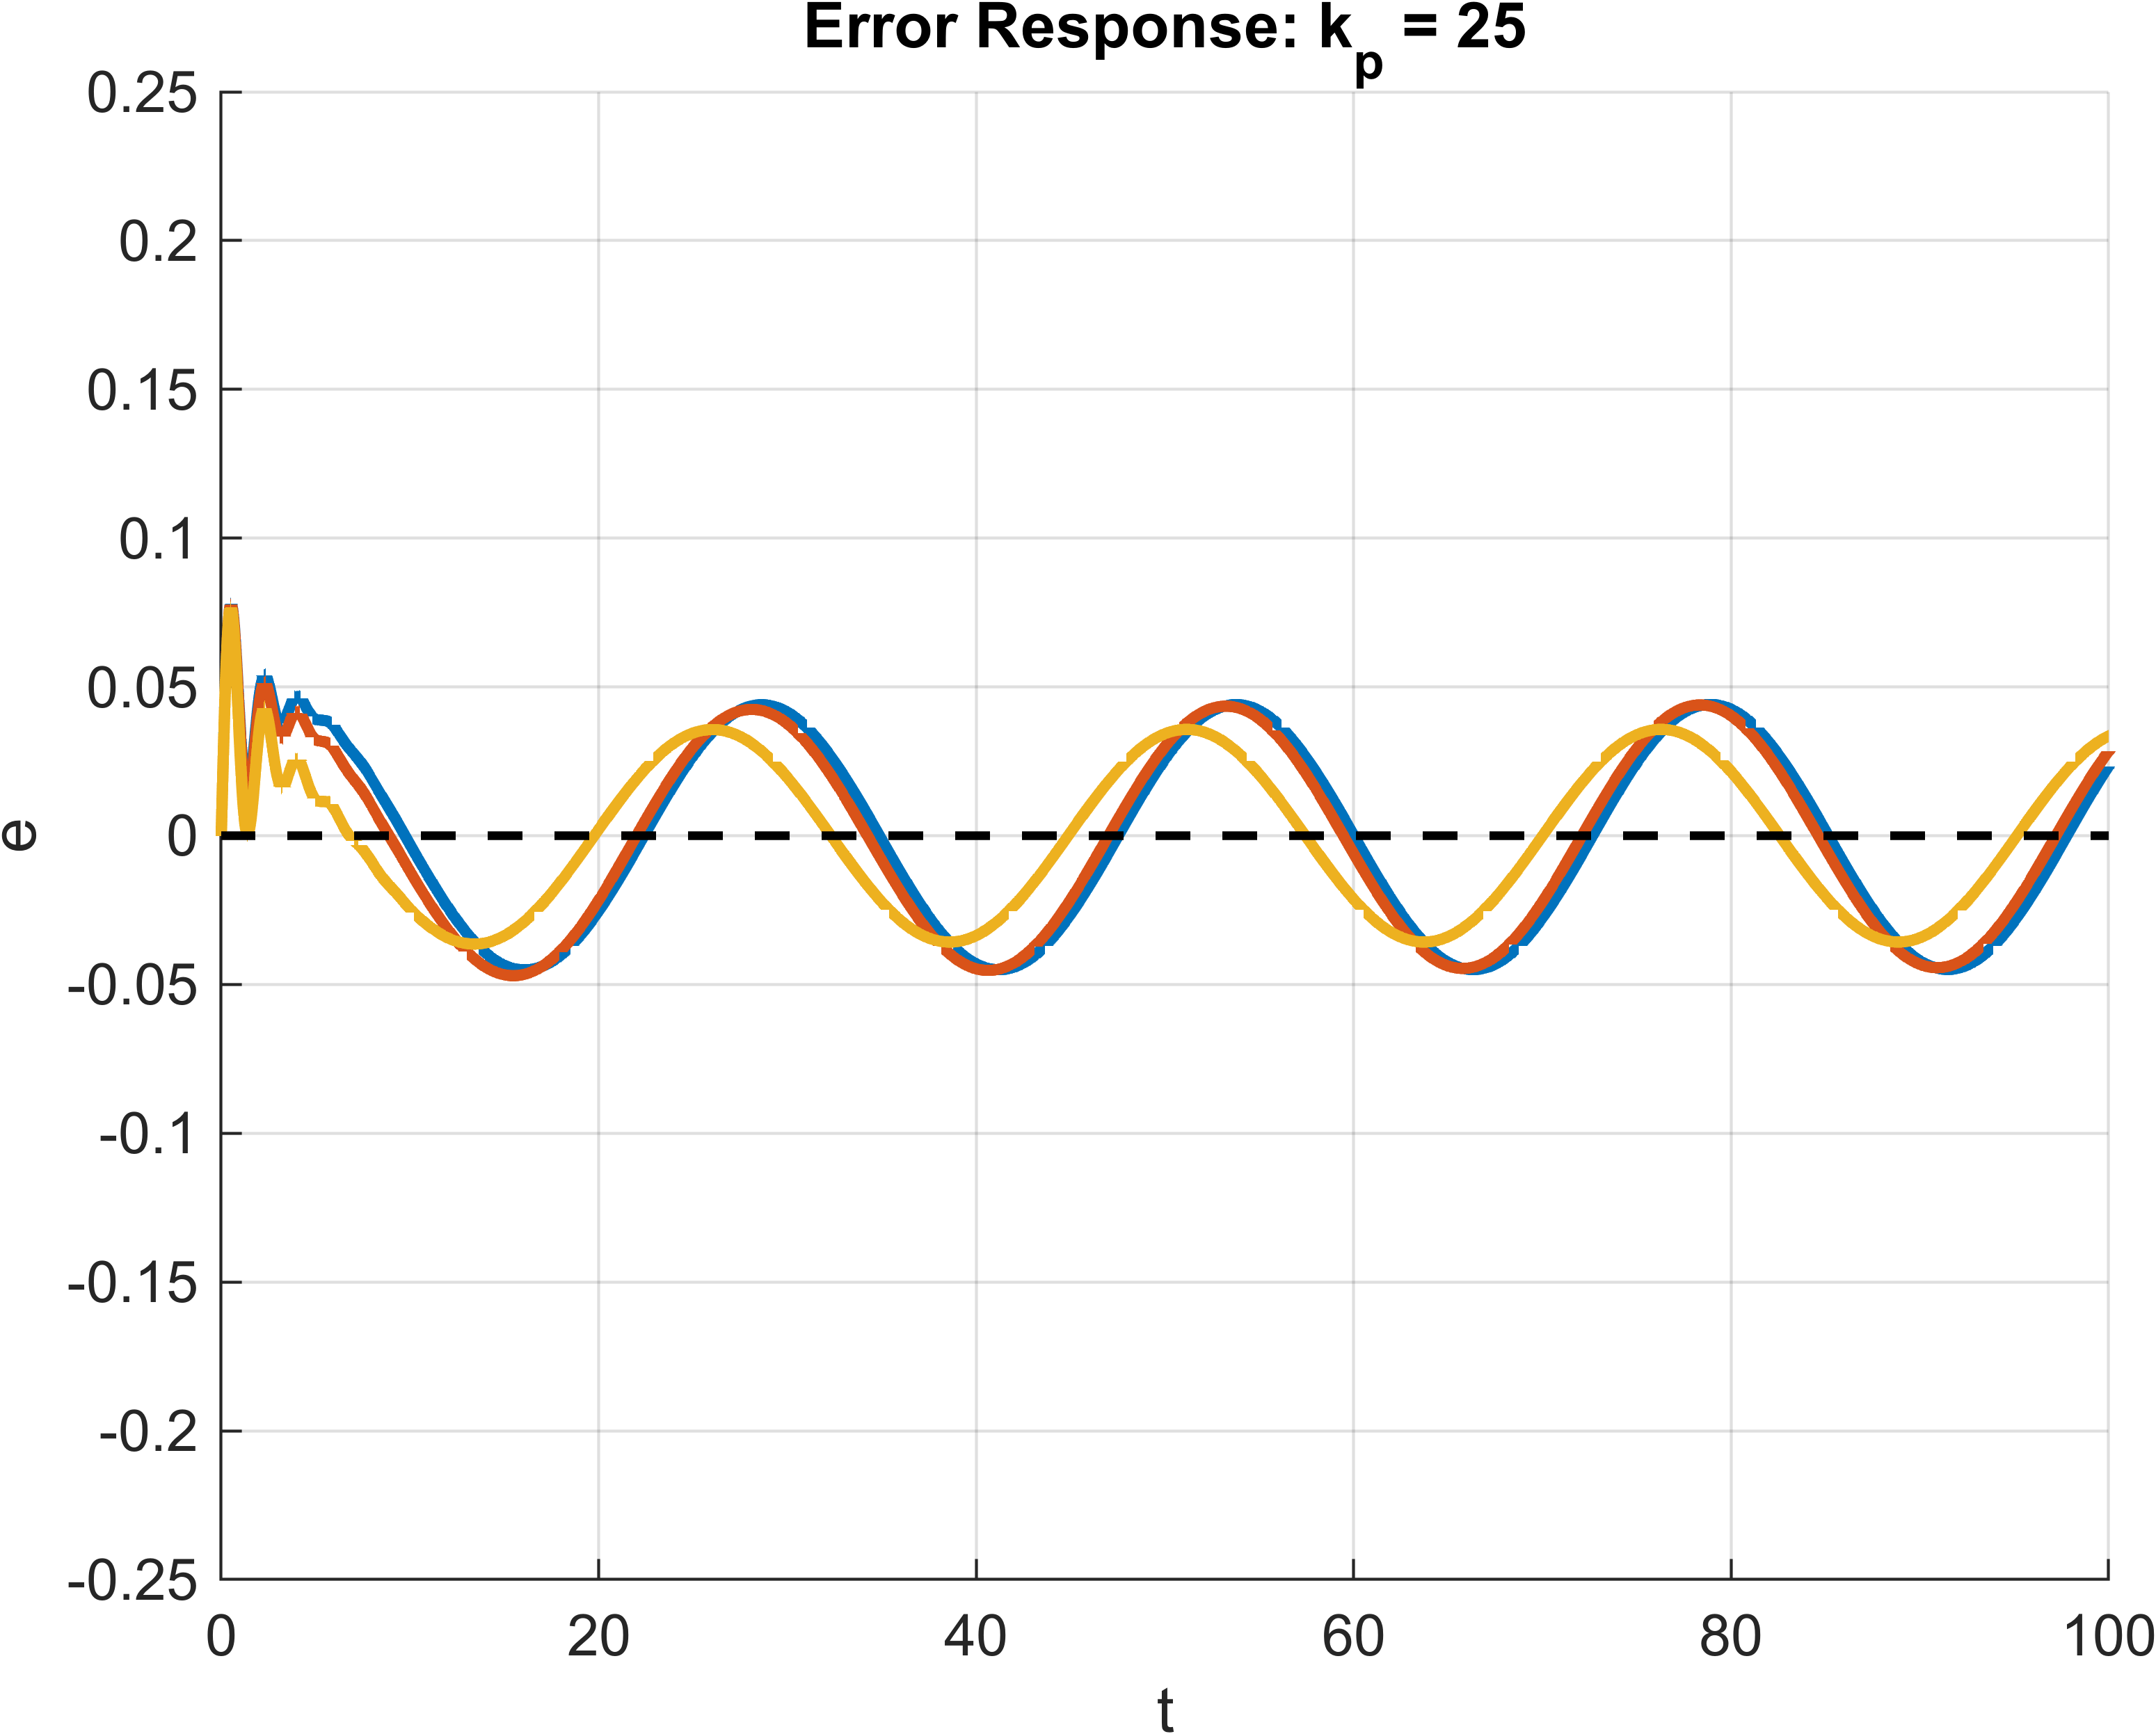
\includegraphics[width=1\textwidth, trim={1cm 0cm 1cm 0cm}]{../images/input_4_kp_25_error.png}
    \end{minipage}
    \caption{Графики $y(t)$ и $e(t)$ при $g(t) = \sin(0.25t)$ и $k_p = 25$}
\end{figure}

Как видно из графиков, ПИ-регулятор не может обеспечить 
слежение за гармоническим сигналом. Ошибка имеет гармонический характер.
Увеличение коэффициентов $k_p$ и $k_i$ уменьшает амплитуду ошибки.
\endinput

\chapter{Вывод}
В ходе выполнения лабораторной работы были изучены методы стабилизации
для систем с идеальным и реальными дифференцирующими звеньями. Были
рассмотрены П, И, ПИ регуляторы для задачи слежения за четырьмя типами
входных сигналов. Изучено влияние порядка астатизма регуляторов и их
коэффициентов на величину ошибки регулирования.
Также был рассмотрен синтез регулятора общего вида 
для слежения за гармоническим сигналом. 
\endinput
% \printbibliography[title=Список использованных источников] % Автособираемый список литературы

\end{document}